% Start preamble
\documentclass[12pt,a4paper]{article}
\usepackage{geometry}
 \geometry{
 a4paper,
 total={170mm,257mm},
 left=20mm,
 top=20mm,
 }
\usepackage[utf8]{inputenc}
\usepackage[T1]{fontenc}
\usepackage[pdftex]{graphicx}
\graphicspath{{./}}
\usepackage{enumitem}
\usepackage{pdfpages}
\usepackage{hyperref}
\usepackage{tikz}
\usepackage{attachfile}
\usepackage{epstopdf}
%\usepackage[table]{xcolor,colorbl}
\usepackage{array}
\setlength{\textwidth}{16cm}
\setlength{\oddsidemargin}{-0.5cm}
\setlength{\evensidemargin}{-0.5cm}
%\setlenght{\headsep}{0cm}
\setlength\parindent{0pt}
%\setlength{\extrarowheight}{3pt}
%%%%%% Counting oppgaves %%%%%%
 \newcount\questnum \questnum=0
 \def\oppgave{
            \advance\questnum by 1
            \ifnum \questnum > 0
                 \hrule
                 \vskip 3pt
                 \leftline{Oppgave \the\questnum}
                 \vskip 3pt \fi}
 %%%%%%%%%%%%%%%%%%%%%%
%%%%%%%%%%%%%%%%%%%%%%


%%%%%% Counting answers %%%%%%
\newcount\answnum \answnum=0
\def\svar{
           \advance\answnum by 1
           \ifnum \answnum > 0
                \hrule
                \vskip 3pt
                \leftline{Svar \the\answnum}
                \vskip 3pt \fi}
%%%%%%%%%%%%%%%%%%%%%%


%%%%%% Counting notes %%%%%%
\newcount\explnum \explnum=0
\def\notes{
           \advance\explnum by 1
           \ifnum \explnum > 0
                \hrule
                \vskip 3pt
                \leftline{Notes \the\explnum}
                \vskip 3pt \fi}
%%%%%%%%%%%%%%%%%%%%%%

% End preamble

\begin{document}
% !TEX root = /home/fred-olav/afgv/src/preamble.tex
\centerline{\bf Strømningsmålling}  \bigskip

Kompetansemål:
\begin{itemize}[noitemsep]

	\item montere, konfigurere, kalibrere og idriftsettelse digitale og analoge målesystemer
	\item måle fysiske størrelser i automatiserte anlegg
\end{itemize}
% til neste år må rangeability med
%	Forkunnskaper
\vskip 2cm

\noindent \underbar{Del 1}

\vskip 5pt

%INSTRUCTOR \noindent {\bf Problem-solving intro activity:} review INST241\_x1 exam.

\vskip 2pt \noindent {\bf Emne for lekesjonen:} Teknologier for flowmåling

\vskip 2pt \noindent Oppgave 1 - 20; \underbar{besvar oppgave 1-10} som forberedelse til leksjon %(remainder for practice)

\vskip 10pt

	Læringsmål:
	Målet for leksjonen er å gi en oversikt ovre ulike måleprinsipper som brukes for å måle strømning. 
	\begin{itemize}[noitemsep]
		\item Kunne navngi og beskrive virkemåte for ulike måleelementer som brukes i trykkbaserte strømningsmålere.% Venturirør, måleblende, pitotrør, annubar
		\item Kunne navngi og beskrive virkemåte for ulike måleprinsipper for hastighetsbaserte strømningsmålere.
		\item Kunne forklare måleprinsippet til en Coriolis strømningsmåler
		\item Kunne forklare måleprinsippet til fortrengingsmålere
		\item Kunne forklare måleprinsippet til termiske strømningsmålere. 
	\end{itemize}


%%%%%%%%%%%%%%%
\filbreak
\hrule \vskip 5pt
\noindent \underbar{Del 2}

\vskip 5pt

%INSTRUCTOR \noindent {\bf Problem-solving intro activity:} explore the ``curved arrow'' notation for voltage in DC circuits shown in the ``Electrical Sources and Loads'' section of the ``DC Electricity'' chapter of the LIII textbook, commenting on how this notation is analagous to force and displacement, helping to explain positive and negative quantities of mechanical work.

\vskip 2pt \noindent {\bf Emne for leksjonen:} Fluid dynamikk

\vskip 2pt \noindent Oppgave 21 - 40; \underbar{besvar oppgave 21-30} som forberedelse til leksjonen%(remainder for practice)

\vskip 10pt

	Målet for leksjonen er å bygge en intuisjon for hvordan fluider strømer i rør ved å regne på ulike eksempler. 

	Læringsmål:
	\begin{itemize}[noitemsep]
		\item Kunne forklar hva viskositet er og hvilken enhet absolutt viskositet måles i 
		\item Kunne forklare hva Reynolds nummer og regne ut dette for strømning i rør.
		\item Kunne forklare forskjellen på turbulent og laminær strømning
		\item Kunne forklare og bruke Law of Continuity 
		\item Kunne forklare og bruke Bernoullis formel
	\end{itemize}


%%%%%%%%%%%%%%%
\filbreak
\hrule \vskip 5pt
\noindent \underbar{Del 3}

\vskip 5pt

%INSTRUCTOR \noindent {\bf Problem-solving intro activity:} apply the critical reading strategy suggested in Question 0 where readers are encouraged to work through mathematical exercises.  A specific example of this would be to verify the square-root scales of indicator gauges shown in the textbook using a calculator, correlating equivalent values shown on the linear versus square-root scales.

\vskip 2pt \noindent {\bf Emne for leksjonen:} Trykkbaserte strømningsmålere

\vskip 2pt \noindent Oppgave 41 - 60; \underbar{besvar oppgave 41-50} som forberedelse til leksjonen%(remainder for practice)

\vskip 10pt


	Målet for leksjonen er å gi en oversikt over trykkbaserte strømningsmålere, hvordan disse installeres og at disse krever kvadratrotuttrekker. 

	Læringsmål:
	\begin{itemize}[noitemsep]
		\item Kunne forklare forskjellen på volumentrisk strømning og massestrømning.
		\item Kunne forklare hva som menes med kvadratrotuttrekker og regne med signalstyre inn og ut av en kvadratrotuttrekker.
		\item Kunne beskrive riktig installasjon av trykkbaserte stømningsmålere.
		\item Kunne regne på oppgaver med strømningn i trykkbaserte strømningsmålere. 
	\end{itemize}


%%%%%%%%%%%%%%%
\filbreak
\hrule \vskip 5pt

\noindent \underbar{Del 4}

\vskip 5pt

%%%%%INSTRUCTOR \noindent {\bf Problem-solving intro activity:} Research equipment manuals to sketch a complete circuit connecting a loop controller to either a 4-20 mA transmitter or a 4-20 mA final control element ({\tt i03773})

%%%%%INSTRUCTOR \noindent {\bf Problem-solving intro activity:} identifying possible ways in which an orifice-based flowmeter can give false readings.  Refer to the P\&ID in {\tt i03490} for examples, such as nitrogen flowmeter FT-29 or steam flowmeter FT-28.

\vskip 2pt \noindent {\bf Emne for leksjonen:} Hastighetsbasert strømningsmålere

\vskip 2pt \noindent Oppgave 61 - 90; \underbar{besvar oppgave 61-70} som forberedelse til leksjonen%(remainder for practice)

%\vskip 5pt

Målet for leksjonen er å gi en oversikt over måleprinsippene for hastighetsbaserte strømningsmålere.

	Læringsmål:
	\begin{itemize}[noitemsep]
		\item Kunne installere og regne ut k-verdi for turbin strømningsmåler
		\item Kunne installere og renge ut k-verdi for vortex strømningsmålere. 
		\item Kunne installere magnetiske strømningsmålere
		\item Kunne installere ultralyd strømningsmålere. 
	\end{itemize}

%\noindent Feedback questions {\it (81 through 90)} are optional and may be submitted for review at the end of the day
%
%\vskip 10pt

\filbreak
\hrule \vskip 5pt
\noindent \underbar{Del 5} 

\vskip 5pt

%INSTRUCTOR \noindent {\bf Problem-solving intro activity:} identifying possible/impossible faults in a flow measurement loop using either a turbine, vortex, or positive displacement flowmeter, referencing a P\&ID (e.g. from the {\it Realistic Instrumentation Diagrams} practice worksheet)

\vskip 2pt \noindent {\bf Emne for leksjonen:} Andre strømningsmålere. 

\vskip 2pt \noindent Oppgave 91-120; \underbar{besvar oppgave 91-99} som forberedelse til laksjonen (remainder for practice)

\vskip 10pt


Målet for leksjonen er å gi en oversikt over måleprinsippene for ulike strømningsmålere som ikke kommer inn under de andre kateboriene.

	Læringsmål:
	\begin{itemize}[noitemsep]
		\item  Kunne installere coriolis strømningsmålere. 
	\end{itemize}

%%%%%%%%%%%%%%%
\vfil \eject
\vfil \eject
\centerline{\bf Oppgaver}
\vskip 5pt
\oppgave{} 
% Copyright 2009, Tony R. Kuphaldt, released under the Creative Commons Attribution License (v 1.0)
% This means you may do almost anything with this work of mine, so long as you give me proper credit


Skummles "Continuous Fluid flow Measurment" kapittelet i afgv.pdf for spesifikt å besvare disse spørsmålene:
%Skim the ``Continuous Fluid Flow Measurement'' chapter in your {\it Lessons In Industrial Instrumentation} textbook to specifically answer these questions:

\vskip 10pt

Trykkbaserte strømningsmålere virker med å tvinge et fluid til å \textit{akselerere} eller \textit{deakselerere} mens det strømmer igjennom et rør. Dette gjør at det oppstår en trykkforsjell. Plukk ut noen av de forskjellige måleelementene (metoder) som brukes til å skape denne akselerasjonen eller deakselerasjonen. (hint. Venturirør er et eksempel)
%Pressure-based flowmeters work by forcing the fluid to {\it accelerate} or {\it decelerate} as it flows through a pipe, which causes a static pressure difference to develop.  Identify some of the different {\it flow elements} used to create the acceleration/deceleration inside a pipe (hint: a ``venturi tube'' is one example of a flow element creating a pressure differential).

\vskip 10pt
For hvert ev måleelementene finn ut om de virker med å akselerere eller deakselerere fluidet. Forklar hvorfor du tror det. 
%For each of the flow elements you identify, determine whether it works by fluid acceleration or by fluid deceleration, and explain your reasoning.

\vskip 10pt

I hvilken del av måleelementet er trykket størst, der hvor hastigheten er størst eller der hvor hastigheten er minst. (Hint. så på hvordan DP-cellen er tilkoblet. )
%In which region of a flow element is the pressure greatest, the region of {\it greatest velocity} or the region of {\it least velocity}?  Hint: the orientation of the DP transmitter's ``H'' and ``L'' ports is a clue!


\vskip 20pt \vbox{\hrule \hbox{\strut \vrule{} {\bf Suggestions for Socratic discussion} \vrule} \hrule}

\begin{itemize}
\item{} Identify different strategies for ``skimming'' a text, as opposed to reading that text closely.  Why do you suppose the ability to quickly scan a text is important in this career?
\end{itemize}

\underbar{file i04020}
\vskip 10pt \filbreak 
\oppgave{} 
% Copyright 2009, Tony R. Kuphaldt, released under the Creative Commons Attribution License (v 1.0)
% This means you may do almost anything with this work of mine, so long as you give me proper credit

Skummles "Continuous Fluid flow Measurment" kapittelet i afgv.pdf for spesifikt å besvare disse spørsmålene:

\vskip 10pt

To vanlige typer av "variabelt areal" strømningsmwler er \textit{rotameter } og \textit{Weirs}. Forklar hvordan hver av disse strømningsmålerene virker, og nøyaktiv hvor strømningsarealet varierer ettersom strømningsraten øker eller minker. 
%Two common styles of ``variable area'' flowmeter are {\it rotameters} and {\it weirs}.  Explain how each one of these flowmeter types functions, and where (exactly) is the flow-path area varying as flow rate increases and decreases.

\vskip 10pt

%Describe the difference between a {\it weir} and a {\it flume}, and identify a practical application in industry where either one of these flow elements might be used.


\vskip 20pt \vbox{\hrule \hbox{\strut \vrule{} {\bf Suggestions for Socratic discussion} \vrule} \hrule}

\begin{itemize}
\item{} Identify different strategies for ``skimming'' a text, as opposed to reading that text closely.  Why do you suppose the ability to quickly scan a text is important in this career?
\end{itemize}

\underbar{file i04021}
\vskip 10pt \filbreak 
\oppgave{} 
% Copyright 2009, Tony R. Kuphaldt, released under the Creative Commons Attribution License (v 1.0)
% This means you may do almost anything with this work of mine, so long as you give me proper credit


Skummles "Continuous Fluid flow Measurment" kapittelet i afgv.pdf for spesifikt å besvare disse spørsmålene:
\vskip 10pt

Forklar hvordan et turbinflowmeter måler hastigheten til et fluid når strømmer igjennom et rør. 

\vskip 10pt


Forklar hva {\it von K\'arm\'an} effekten er, og hvordan den kan utnyttet til å måle hastigheten til  en gass eller en væske. 

\vskip 10pt

Forklar hvordan en elektromagnetisk strømningmåler måler hastigheten til et fluid. 

\vskip 10pt

Forklar hverdan en ultralyd strømningsmåler måler hastigheten til et fluid. 
\vskip 10pt

Explain how an {\it optical} flowmeter measures fluid velocity.
Forklar hvordan et optisk flowmeter måler hastigheten til et fluid. 

\vskip 20pt \vbox{\hrule \hbox{\strut \vrule{} {\bf Suggestions for Socratic discussion} \vrule} \hrule}

\begin{itemize}
\item{} Identify different strategies for ``skimming'' a text, as opposed to reading that text closely.  Why do you suppose the ability to quickly scan a text is important in this career?
\end{itemize}

\underbar{file i04022}
\vskip 10pt \filbreak 
\oppgave{} 
% Copyright 2009, Tony R. Kuphaldt, released under the Creative Commons Attribution License (v 1.0)
% This means you may do almost anything with this work of mine, so long as you give me proper credit

Skummles "Continuous Fluid flow Measurment" kapittelet i afgv.pdf for spesifikt å besvare disse spørsmålene:

\vskip 10pt
Positiv fortrenings strømningsmålere har beveglige deler for å måle når et fluid passerer igjennom dem, de skiller seg likevell fra andre strømningsmålere med beveglige deler (som f.eks. turbinmeter). Forklar hva som er anderledes med positiv fortrengings strømningsmålere. 
%Positive displacement flowmeters have moving parts inside to measure the passage of fluids through them, yet they are different from other flowmeter types using moving parts (such as turbine meters).  Explain what is different about a ``positive displacement'' flowmeter.


\vskip 20pt \vbox{\hrule \hbox{\strut \vrule{} {\bf Suggestions for Socratic discussion} \vrule} \hrule}

\begin{itemize}
\item{} Identify different strategies for ``skimming'' a text, as opposed to reading that text closely.  Why do you suppose the ability to quickly scan a text is important in this career?
\end{itemize}

\underbar{file i04025}
\vskip 10pt \filbreak 
\oppgave{} 
% Copyright 2009, Tony R. Kuphaldt, released under the Creative Commons Attribution License (v 1.0)
% This means you may do almost anything with this work of mine, so long as you give me proper credit

Skummles "Continuous Fluid flow Measurment" kapittelet i afgv.pdf for spesifikt å besvare disse spørsmålene:

\vskip 10pt

En spesiell type strømningsmåler er \textit{Corilis}-strømningsmåler. Forklar så godt du kan hvordan denne type strømningsmåler virker. 
%One of the stranger flow-measurement technologies is the {\it Coriolis} flowmeter.  Do your best to explain how this type of flowmeter functions. 


\vskip 20pt \vbox{\hrule \hbox{\strut \vrule{} {\bf Suggestions for Socratic discussion} \vrule} \hrule}

\begin{itemize}
\item{} Identify different strategies for ``skimming'' a text, as opposed to reading that text closely.  Why do you suppose the ability to quickly scan a text is important in this career?
\end{itemize}

\underbar{file i04023}
\vskip 10pt \filbreak 
\oppgave{} 
% Copyright 2009, Tony R. Kuphaldt, released under the Creative Commons Attribution License (v 1.0)
% This means you may do almost anything with this work of mine, so long as you give me proper credit

Skummles "Continuous Fluid flow Measurment" kapittelet i afgv.pdf for spesifikt å besvare disse spørsmålene:


\vskip 10pt

Det føles kaldere ute når det blåser, forklar hvordan dette prinsippet kan brukes til å måle hastigheten til et fluid i et rør. 
%A cold day ``feels colder'' if a strong wind is blowing.  Describe how this principle may be exploited to measure the velocity of a fluid flowing through a pipe. 

\vskip 10pt

Ut fra de måtene du vet at varme kan overføres, hvilken brukes av temiske flowmeter? \textit{varmeleding}, \textit{konveksjon} eller, \textit{varmestråling}. 
%Based on what you know of modes of heat transfer, is the operating principle of a thermal flowmeter based on {\it conduction}, {\it convection}, or {\it radiation}?


\vskip 20pt \vbox{\hrule \hbox{\strut \vrule{} {\bf Suggestions for Socratic discussion} \vrule} \hrule}

\begin{itemize}
\item{} Identify different strategies for ``skimming'' a text, as opposed to reading that text closely.  Why do you suppose the ability to quickly scan a text is important in this career?
\end{itemize}

\underbar{file i04024}
\vskip 10pt \filbreak 
\oppgave{} 
% Copyright 2009, Tony R. Kuphaldt, released under the Creative Commons Attribution License (v 1.0)
% This means you may do almost anything with this work of mine, so long as you give me proper credit

Skummles "Continuous Fluid flow Measurment" kapittelet i afgv.pdf for spesifikt å besvare disse spørsmålene:


\vskip 10pt

Describe what a {\it weighfeeder} is, and what sort of process material flowrate it is designed to measure.


\vskip 20pt \vbox{\hrule \hbox{\strut \vrule{} {\bf Suggestions for Socratic discussion} \vrule} \hrule}

\begin{itemize}
\item{} Identify different strategies for ``skimming'' a text, as opposed to reading that text closely.  Why do you suppose the ability to quickly scan a text is important in this career?
\end{itemize}

\underbar{file i04026}
\vskip 10pt \filbreak 
\oppgave{} 
% Copyright 2009, Tony R. Kuphaldt, released under the Creative Commons Attribution License (v 1.0)
% This means you may do almost anything with this work of mine, so long as you give me proper credit

Skim the ``Continuous Fluid Flow Measurement'' chapter in your {\it Lessons In Industrial Instrumentation} textbook to specifically answer these questions:

\vskip 10pt

You have already explored how {\it load cells} may be used to infer the amount of material stored in process vessels.  Explain how these same devices may be used to infer flowrate in and out of the same vessels using the {\it change-of-quantity} technique.

\vskip 10pt

Suppose an instrument technician decides to build a flowmeter for her propane-fueled barbecue, by placing the propane fuel tank on top of an electronic weigh scale (like a standard bathroom scale).  Explain how the technician could take the measurements given by this scale and somehow convert them to register as a {\it flowrate} of propane gas.


\vskip 20pt \vbox{\hrule \hbox{\strut \vrule{} {\bf Suggestions for Socratic discussion} \vrule} \hrule}

\begin{itemize}
\item{} Identify different strategies for ``skimming'' a text, as opposed to reading that text closely.  Why do you suppose the ability to quickly scan a text is important in this career?
\end{itemize}

\underbar{file i04027}
\vskip 10pt \filbreak 
\oppgave{} 
% Copyright 2009, Tony R. Kuphaldt, released under the Creative Commons Attribution License (v 1.0)
% This means you may do almost anything with this work of mine, so long as you give me proper credit

Read and outline the ``Work, Energy, and Power'' subsection of the ``Classical Mechanics'' section of the ``Physics'' chapter in your {\it Lessons In Industrial Instrumentation} textbook.  Note the page numbers where important illustrations, photographs, equations, tables, and other relevant details are found.  Prepare to thoughtfully discuss with your instructor and classmates the concepts and examples explored in this reading.

\underbar{file i04028}
\vskip 10pt \filbreak 
\oppgave{} 
% Copyright 2009, Tony R. Kuphaldt, released under the Creative Commons Attribution License (v 1.0)
% This means you may do almost anything with this work of mine, so long as you give me proper credit

Calculate the amount of potential energy stored in the mass of an elevator plus its cargo of potatoes (570 pounds) as it lifts up to a height of 10 feet.  Express this potential energy in both British and metric units.  Also, identify which equation is more convenient to use for this calculation: $E_p = Fx$ or $E_p = mgh$?

\vskip 10pt

Calculate the kinetic energy of a bullet with a mass of 150 grains (9.7198 grams) traveling at a velocity of 2820 feet per second, expressing your answer in both British and metric units.

\vskip 20pt \vbox{\hrule \hbox{\strut \vrule{} {\bf Suggestions for Socratic discussion} \vrule} \hrule}

\begin{itemize}
\item{} Demonstrate how to {\it estimate} numerical answers for this problem without using a calculator.
\item{} Describe the various energy-transfer operations taking place when a crane lifts a heavy weight and then sets it down in a different location.
\item{} If a crane lifts a weight 10 feet above the ground, then sets that weight down on top of an object 6 feet above the ground, is energy still conserved?  Explain in detail.
\item{} Identify how to secure a crane in a zero-energy state prior to performing maintenance work on it.
\item{} Which has a greater effect on a moving object's kinetic energy: an increase in mass or an increase in velocity?
\item{} If an automobile doubles its speed, how much longer (distance) will it take to skid to a complete stop if the driver suddenly applies the brakes?
\end{itemize}

\underbar{file i04029}
\vskip 10pt \filbreak 
\oppgave{} 
% Copyright 2006, Tony R. Kuphaldt, released under the Creative Commons Attribution License (v 1.0)
% This means you may do almost anything with this work of mine, so long as you give me proper credit

Den etablerte måleblenden er en av mange forskjellige måleelementer som virker ved å generere en trykkforskjell. Forklar kort hvordan hvert av disse måleelementene virker. 
%The venerable {\it orifice plate} is but one of many different pressure-generating primary sensing elements (PSE's) for flow measurement.  Briefly describe how each of these flow PSEs work, and how they compare against orifice plates in terms of application and performance:

$$\includegraphics[width=15.5cm]{i00479x01.eps}$$

\vskip 10pt

$$\includegraphics[width=15.5cm]{i00479x02.eps}$$

\vskip 10pt

$$\includegraphics[width=15.5cm]{i00479x03.eps}$$

\vskip 10pt

$$\includegraphics[width=15.5cm]{i00479x04.eps}$$

\vskip 10pt

$$\includegraphics[width=15.5cm]{i00479x05.eps}$$

\vskip 10pt

$$\includegraphics[width=15.5cm]{i00479x06.eps}$$

\vskip 10pt

$$\includegraphics[width=15.5cm]{i00479x07.eps}$$

\vskip 10pt

$$\includegraphics[width=15.5cm]{i00479x08.eps}$$

\underbar{file i00479}
\vskip 10pt \filbreak 
\oppgave{} 
% Copyright 2006, Tony R. Kuphaldt, released under the Creative Commons Attribution License (v 1.0)
% This means you may do almost anything with this work of mine, so long as you give me proper credit


Michael Faraday, den berømte Engelsek fysikeren, prøvde en gang å elektrisk måle strømingen i elven Themsen. Teknikkenhans, som ikke virket, var basert på at en ledende væske beveger seg igennom et magnetfelt. Forklar hva Michael Faraday gjorde og hvordan vi kan bruke denne teknikken til å måle strømningen i et rør.

%Michael Faraday, the famous English physicist, once attempted to {\it electrically} measure the flow rate of the Thames river.  His technique, unsuccessful as it was, was based on the idea of a fluid conductor moving perpendicular to a magnetic field.  Explain what Michael Faraday did and how we may apply this technique (successfully!) to the measurement of fluids in pipes.

\underbar{file i00522}
\vskip 10pt \filbreak 
\oppgave{} 
% Copyright 2006, Tony R. Kuphaldt, released under the Creative Commons Attribution License (v 1.0)
% This means you may do almost anything with this work of mine, so long as you give me proper credit

Noen dyr bruker ekkolokasjon for å finne veien i mørket. Ubåter bruker sonar til det samme. Forklar hvordan dette prinsippet kan brukes til å akustisk måle avstanden til et objekt. Hvordan kan vi bruke dette til å måle hastigheten til et objekt?
%Some animals use the principle of {\it echo-location} to find their way in the dark, where there is too little light to effectively use their eyes.  Submarines use {\it sonar} to do the same thing.  Explain how the same principle works to acoustically determine distance of a solid object, then determine how the same principle could be extended to determine the {\it speed} of a solid object.

\underbar{file i00528}
\vskip 10pt \filbreak 
\oppgave{} 
% Copyright 2006, Tony R. Kuphaldt, released under the Creative Commons Attribution License (v 1.0)
% This means you may do almost anything with this work of mine, so long as you give me proper credit

Hva menes med massestrøm sett i forhold til volumstrøm?
%What is meant by the phrase ``mass flow measurement,'' especially as it compares to ``volumetric flow measurement?''  In other words, what is the practical difference between measuring flow rate in units of mass per time versus units of volume per time?

\underbar{file i00499}
\vskip 10pt \filbreak 
\oppgave{} 
% Copyright 2006, Tony R. Kuphaldt, released under the Creative Commons Attribution License (v 1.0)
% This means you may do almost anything with this work of mine, so long as you give me proper credit

På kalde dager, blir følelsen av temperatur forstyrret om det blåser. Selv om et thermometer ikke vil vise lavere temperatur når det blåser, så føles det kaldere. Denne effekten bruke av i værmeldinger som føles som temperatur. 

%On cold days, the perception of ambient temperature becomes skewed with the presence of any substantial wind speed.  Although a thermometer will not register a colder temperature if the wind blows, it certainly {\it feels} colder when the wind blows!  This effect is commonly known as {\it wind chill}.

Den samme effekten kan brukes til å måle massestrømning. Strømningsmålere basert på dette prinsippet kalles terminsk strømningsmåler. Forklar hvordan termiske strømningsmålere er konstruert. 
%This same effect may be exploited to measure mass flow.  Flowmeters based on this principle are called {\it thermal} mass flowmeters.  Explain how a thermal mass flowmeter is constructed, and identify any physical properties of the fluid stream that will affect its calibration.

\underbar{file i00534}
\vskip 10pt \filbreak 
\oppgave{} 
% Copyright 2006, Tony R. Kuphaldt, released under the Creative Commons Attribution License (v 1.0)
% This means you may do almost anything with this work of mine, so long as you give me proper credit

Coriolis massestrømningsmålere har flere fordeler over andre strømingsmålere. Dette gjør at det ofte er verdt den høye kostnaden som er forbundet med anskaffelse. List opp noen av fordelen og eventuelt ulamper med denne teknologien.  
%Coriolis-effect mass flowmeters have several advantages over other mass-flow technologies, which make them worth their high price in some applications.  Identify what some of these advantages are.  Also, identify some of their outstanding disadvantages (besides relatively high cost).

\underbar{file i00539}
\vskip 10pt \filbreak 
\oppgave{} 
% Copyright 2006, Tony R. Kuphaldt, released under the Creative Commons Attribution License (v 1.0)
% This means you may do almost anything with this work of mine, so long as you give me proper credit

Det er et problem en eller annen plass i dette væskestrømningsreguleringssystemet. Regulatoren er i auto-modus, med et settpunkt på  65\%, men likevell viser FT og FIC 0.3\% (nesten ingen strømning). 
%There is a problem somewhere in this liquid flow control system.  The controller is in automatic mode, with a setpoint of 65\%, yet the flow indicator and the flow controller both register 0.3\%: (nearly) zero flow.  A P\&ID of the loop appears here:

$$\includegraphics[width=15.5cm]{i02518x01.eps}$$

Forklar hvordan du ville feilsøkt i dette systemet, og hvilke mulige feil som kan forårsake at regulatorn ikke klarer å holde settpunktet. 

%Explain how you would begin troubleshooting this system, and what possible faults could account for the controller not being able to maintain liquid flow at setpoint.

\vskip 20pt \vbox{\hrule \hbox{\strut \vrule{} {\bf Suggestions for Socratic discussion} \vrule} \hrule}

\begin{itemize}
\item{} Explain how you could divide this control system into distinct areas or zones which you may then begin to refer to when ``dividing and conquering'' the problem. 
\end{itemize}

\underbar{file i02518}
\vskip 10pt \filbreak 
\oppgave{} 



%\vfil

%\underbar{file i00000}
%\eject
\vskip 10pt \filbreak 
\oppgave{} 



%\vfil

%\underbar{file i00000}
%\eject
\vskip 10pt \filbreak 
\oppgave{} 



%\vfil

%\underbar{file i00000}
%\eject
\vskip 10pt \filbreak 
\oppgave{} 
% Copyright 2009, Tony R. Kuphaldt, released under the Creative Commons Attribution License (v 1.0)
% This means you may do almost anything with this work of mine, so long as you give me proper credit

Les og understrek afgv.pdf/Phusices/Fluid Mechanics/Fluid Viscosity  kapittelet. Noter sidenummer med viktige illustasjoner, bilder, formler og annen viktig informasjon. Forbered deg på å kunne diskutere emnet fluid viskositet. 

\underbar{file i04030}
\vskip 10pt \filbreak 
\oppgave{} 
% Copyright 2009, Tony R. Kuphaldt, released under the Creative Commons Attribution License (v 1.0)
% This means you may do almost anything with this work of mine, so long as you give me proper credit

Les og understrek afgv.pdf/Phusices/Fluid Mechanics/Reynolds Number. Noter sidenummer med viktige illustasjoner, bilder, formler og annen viktig informasjon. Forbered deg på å kunne diskutere emnet fluid viskositet. 


\underbar{file i04031}
\vskip 10pt \filbreak 
\oppgave{} 
% Copyright 2009, Tony R. Kuphaldt, released under the Creative Commons Attribution License (v 1.0)
% This means you may do almost anything with this work of mine, so long as you give me proper credit

Les og understrek afgv.pdf/Phusices/Fluid Mechanics/Law of Continuity. Noter sidenummer med viktige illustasjoner, bilder, formler og annen viktig informasjon. Forbered deg på å kunne diskutere emnet fluid viskositet. 

\underbar{file i04032}
\vskip 10pt \filbreak 
\oppgave{} 
% Copyright 2009, Tony R. Kuphaldt, released under the Creative Commons Attribution License (v 1.0)
% This means you may do almost anything with this work of mine, so long as you give me proper credit

Vi har et rør som det strømmer olje med en strømningsrate på 120 m³/h og en temperatur på 50°C. Begge seksjonene er etter schedule 40.  Den første delen av røret har dimensjon DN200 (ID=202.74mm) og den andre delen har dimensjon DN65 (ID=62.68mm)

$$\includegraphics[width=15.5cm]{i04033x01.eps}$$

Regn ut hastigheten for fluidet i røret h hver av seksjonene. Regn også ut den volumentriske strømningsraten i \textit{gallons per minute} (GPM). 


\vskip 10pt

I hvilken seksjon av røret har oljestrømmen høyest reynolds nummer?

\vskip 20pt \vbox{\hrule \hbox{\strut \vrule{} {\bf Suggestions for Socratic discussion} \vrule} \hrule}

\begin{itemize}
\item{} This question is a good application of the {\it Law of Continuity}, but this law is really nothing more than an expression of a more fundamental law in physics.  What is this more fundamental law, and what does it tell us about flow through a pipe?
\item{} Once we know the fluid velocity in one section of the pipe, show how we may calculate the velocity in the other section of the pipe using nothing but a ratio of pipe diameters ($7.981 \over 2.469$), rather than re-calculate the continuity formula again ($v = {Q \over A}$).
\item{} Where along this pipe will individual fluid molecules possess the greatest kinetic energy?
\end{itemize}

Schedule 40 Pipe 8 Inch (DN200 mm)\\
Standard : ANSI/ASME B36.10(Steel Pipe)\\
– Size : NPS 8 Inch\\
– Size : DN200 mm\\
– Inside Dimeter(Pipe ID) : 202.74 mm\\
– Outside Dimeter(Pipe OD) : 219.1 mm\\
– Pipe Wall Thickness : 8.18 mm\\
– Pipe Weight : 42.55 Kilogram per meter (kg/m)\\
– Pipe Weight Including Water : 74.81 Kilogram per meter (kg/m)\\
*NPS = Nominal pipe size(inch) / DN = Diameter nominal(mm)\\
\\\\
Schedule 40 Pipe 2 1/2 Inch (DN65 mm)\\
Standard : ANSI/ASME B36.10(Steel Pipe)\\
– Size : NPS 2 1/2 Inch\\
– Size : DN65 mm\\
– Inside Dimeter(Pipe ID) : 62.68 mm\\
– Outside Dimeter(Pipe OD) : 73 mm\\
– Pipe Wall Thickness : 5.16 mm\\
– Pipe Weight : 8.63 Kilogram per meter (kg/m)\\
– Pipe Weight Including Water : 11.71 Kilogram per meter (kg/m)\\
*NPS = Nominal pipe size(inch) / DN = Diameter nominal(mm)\\
\underbar{file i04033}
\vskip 10pt \filbreak 
\oppgave{} 
% Copyright 2009, Tony R. Kuphaldt, released under the Creative Commons Attribution License (v 1.0)
% This means you may do almost anything with this work of mine, so long as you give me proper credit

A flowmeter installed in a 6-inch schedule 40 pipe (internal diameter = 6.065 inches) to measure the flow of olive oil requires a Reynolds number of at least 12,500 to function properly.  Calculate the minimum flow rate of oil through this pipe that the flowmeter can measure, assuming the oil's density is 57.3 pounds per cubic foot and its absolute viscosity is 111 centipoise.

\vskip 10pt

Additionally, calculate the minimum average flowing velocity of the olive oil for the flowmeter to properly function.

\vskip 20pt \vbox{\hrule \hbox{\strut \vrule{} {\bf Suggestions for Socratic discussion} \vrule} \hrule}

\begin{itemize}
\item{} How may a piping system be modified to increase the Reynolds number of the flow, for the sake of measuring that flow rate with a flowmeter requiring a high Reynolds number?  Keep in mind that the actual flow rate is fixed here -- we must vary something else to boost Reynolds number for any given flow rate.
\item{} Does the temperature of the liquid have any effect on its Reynolds number?  Why or why not?
\item{} If this pipe were flowing water rather than olive oil, what would the minimum flow rate be to satisfy the Reynolds number requirement of this flowmeter?
\end{itemize}


\underbar{file i04034}
\vskip 10pt \filbreak 
\oppgave{} 
% Copyright 2009, Tony R. Kuphaldt, released under the Creative Commons Attribution License (v 1.0)
% This means you may do almost anything with this work of mine, so long as you give me proper credit

Read and outline the ``Bernoulli's Equation'' subsection of the ``Fluid Mechanics'' section of the ``Physics'' chapter in your {\it Lessons In Industrial Instrumentation} textbook.  Note the page numbers where important illustrations, photographs, equations, tables, and other relevant details are found.  Prepare to thoughtfully discuss with your instructor and classmates the concepts and examples explored in this reading.

\underbar{file i04035}
\vskip 10pt \filbreak 
\oppgave{} 
% Copyright 2009, Tony R. Kuphaldt, released under the Creative Commons Attribution License (v 1.0)
% This means you may do almost anything with this work of mine, so long as you give me proper credit

Read and outline the ``Flow Through a Venturi Tube'' subsection of the ``Fluid Mechanics'' section of the ``Physics'' chapter in your {\it Lessons In Industrial Instrumentation} textbook.  Note the page numbers where important illustrations, photographs, equations, tables, and other relevant details are found.  Prepare to thoughtfully discuss with your instructor and classmates the concepts and examples explored in this reading.

\underbar{file i04036}
\vskip 10pt \filbreak 
\oppgave{} 
% Copyright 2011, Tony R. Kuphaldt, released under the Creative Commons Attribution License (v 1.0)
% This means you may do almost anything with this work of mine, so long as you give me proper credit

Examine this P\&ID and explain how a vacuum is produced in the sour water storage tank (V-10):

$$\includegraphics[width=15.5cm]{i0007rx01.eps}$$

Furthermore, identify what operators would have to do in order to halt the production of vacuum, to make it safe to open an access hatch on V-10 for inspection.  Also, identify how the level of sour water inside the tank is measured.

\vskip 20pt \vbox{\hrule \hbox{\strut \vrule{} {\bf Suggestions for Socratic discussion} \vrule} \hrule}

\begin{itemize}
\item{} Identify how this sour water storage tank is protected against excessive pressure or vacuum, which could rupture it or collapse it, respectively.
\end{itemize}

\underbar{file i03490}
\vskip 10pt \filbreak 
\oppgave{} 
% Copyright 2006, Tony R. Kuphaldt, released under the Creative Commons Attribution License (v 1.0)
% This means you may do almost anything with this work of mine, so long as you give me proper credit

Bruk Bernoulli's formel for å regne ut trykket $P_2$. Massetettheten til fluidet er $\rho = 800kg/m$

%Use Bernoulli's equation to calculate the pressure at the throat of this ``venturi'' tube, assuming water flowing at a rate of 200 liter per sekund, with a weight density ($\gamma$) of 62.4 lb/ft$^{3}$ and a mass density ($\rho$) of 1.951 slugs/ft$^{3}$:

$$\includegraphics[width=15.5cm]{i00452x01.eps}$$

Bernoulli's formel:

\vskip 10pt

$$z_1 \rho g + {v_1^2 \rho \over 2} + P_1 = z_2 \rho g + {v_2^2 \rho \over 2} + P_2$$


\noindent
Where,

$z$ = Height of fluid, in meter (m)

$\rho$ = Mass density of fluid, in kg per kubikkmeter (kg/m$^3$)

$g$ = Acceleration of gravity (9.81 m/s$^{2}$)

$v$ = Hastigheten til fluidet i meter per sekund (m/s)

$P$ = Trykket av fluidet i Pascal (Pa=N/m²) 

\vskip 10pt

Til slutt regn ut differansetrykket i dette venturi måleelementet. ($\Delta P$)

\vskip 10pt

\vskip 20pt \vbox{\hrule \hbox{\strut \vrule{} {\bf Suggestions for Socratic discussion} \vrule} \hrule}

\begin{itemize}
\item{} The textbook outlines a general strategy for generating a problem-solving plan when tackling problems with complex mathematical formulae.  Specifically, this strategy involved writing out the formulae and linking variables between formulae with arrow symbols.  Explain how this strategy works, and show how it may be applied to the solution of this problem.
\item{} A very helpful strategy for tackling Bernoulli's equation problems is to create a table in which to place each of the ``head'' terms of that equation.  Explain why this is helpful to manage this specific type of problem.
\item{} Once we know the velocity of the fluid ($v$) at any point in the tube, is there a way to easily solve for the velocity in any other point in the tube based on a ratio of tube diameters?  For instance, here we know there is a 5:12 ratio of diameters from the throat to the mouth of the tube.  How can we employ this 5:12 ratio to easily determine the velocity at one point (either mouth or throat) knowing the velocity at another?
\end{itemize}

\underbar{file i00452}
\vskip 10pt \filbreak 
\oppgave{} 
% Copyright 2006, Tony R. Kuphaldt, released under the Creative Commons Attribution License (v 1.0)
% This means you may do almost anything with this work of mine, so long as you give me proper credit

Bruk Bernoulli's formel for å regne ut trykket $P_2$. Massetettheten til fluidet er $\rho = 800kg/m$
$$\includegraphics[width=15.5cm]{i00451x01.eps}$$

Bernoulli's formel:

\vskip 10pt

$$z_1 \rho g + {v_1^2 \rho \over 2} + P_1 = z_2 \rho g + {v_2^2 \rho \over 2} + P_2$$

\vskip 10pt

\noindent
Where,

$z$ = Height of fluid, in meter (m)

$\rho$ = Mass density of fluid, in kg per kubikkmeter (kg/m$^3$)

$g$ = Acceleration of gravity (9.81 m/s$^{2}$)

$v$ = Hastigheten til fluidet i meter per sekund (m/s)

$P$ = Trykket av fluidet i Pascal (Pa=N/m²) 

\vskip 10pt

Til slutt regn ut differansetrykket i dette venturi måleelementet. ($\Delta P$)
\vskip 10pt

\vskip 20pt \vbox{\hrule \hbox{\strut \vrule{} {\bf Suggestions for Socratic discussion} \vrule} \hrule}

\begin{itemize}
\item{} The textbook outlines a general strategy for generating a problem-solving plan when tackling problems with complex mathematical formulae.  Specifically, this strategy involved writing out the formulae and linking variables between formulae with arrow symbols.  Explain how this strategy works, and show how it may be applied to the solution of this problem.
\item{} A very helpful strategy for tackling Bernoulli's equation problems is to create a table in which to place each of the ``head'' terms of that equation.  Explain why this is helpful to manage this specific type of problem.
\item{} Venturi tubes are often used to create {\it vacuums}, by passing some fluid through the venturi at high speed and then providing a vacuum tap at the throat.  Automobile engine carburetors and atomizing spray guns are two prominent examples of this.  In industry, another example is the so-called {\it steam eductor}, using a jet of high-velocity steam through a venturi to create continuous suction (vacuum).  Are there any advantages to using eductors to create vacuums as opposed to using mechanical vacuum pumps?  Are there any disadvantages to the use of eductors for creating vacuums?
\end{itemize}

\underbar{file i00451}
\vskip 10pt \filbreak 
\oppgave{} 
% Copyright 2006, Tony R. Kuphaldt, released under the Creative Commons Attribution License (v 1.0)
% This means you may do almost anything with this work of mine, so long as you give me proper credit

As best as possible, define {\it Reynolds number} for a fluid flow using your own words.

\vskip 10pt

Regn ut reynolds nummer for 32 liter vann per sekund (at 20$^{o}$ C) som strømmer i et rør med en diameter på 22 cm. 


\underbar{file i00440}
\vskip 10pt \filbreak 
\oppgave{} 
% Copyright 2006, Tony R. Kuphaldt, released under the Creative Commons Attribution License (v 1.0)
% This means you may do almost anything with this work of mine, so long as you give me proper credit

Jeg kan fylle et kar på 4 liter kjøkken springen på 30 sekunder. Røret til kjøkkenspringen har en ID=12.5mm. Regn ut Reynols tall for denne strømningen. Vil det være turbulent eller laminær stømning?


\underbar{file i00442}
\vskip 10pt \filbreak 
\oppgave{} 
% Copyright 2006, Tony R. Kuphaldt, released under the Creative Commons Attribution License (v 1.0)
% This means you may do almost anything with this work of mine, so long as you give me proper credit

If we poke a hole at the bottom of a vessel containing an otherwise static column of liquid, we have an application for Bernoulli's equation at three different points in the system:

$$\includegraphics[width=15.5cm]{i00446x01.eps}$$

Note that point 1 has no velocity or pressure, but it does have elevation (height); point 2 has no velocity or elevation, but it does have pressure; and point 3 has no elevation or pressure, but it does have velocity.

Use Bernoulli's equation to write a new equation relating the elevation of point 1 with the pressure of point 2 and the velocity of point 3, and then solve for the velocity at point 3 in terms of the other two points' non-zero variables.

\vskip 10pt

\noindent
{\bf Bernoulli's equation:}

$$z_1 \rho g + {v_1^2 \rho \over 2} + P_1 = z_2 \rho g + {v_2^2 \rho \over 2} + P_2$$

\underbar{file i00446}
\vskip 10pt \filbreak 
\oppgave{} 
% Copyright 2006, Tony R. Kuphaldt, released under the Creative Commons Attribution License (v 1.0)
% This means you may do almost anything with this work of mine, so long as you give me proper credit

Regn ut trykket på utløpet av dette røret ($P_2$), om en antar at det strømmer vann ($\rho = 998.19$) og at strømningen skjer uten friksjon.(en får ikke trykktap som følge av friksjon mot rørveggen).  


$$\includegraphics[width=15.5cm]{i00450x01.eps}$$

\vskip 10pt

\noindent
{\bf Bernoulli's equation:}

$$z_1 \rho g + {v_1^2 \rho \over 2} + P_1 = z_2 \rho g + {v_2^2 \rho \over 2} + P_2$$

\vskip 20pt \vbox{\hrule \hbox{\strut \vrule{} {\bf Suggestions for Socratic discussion} \vrule} \hrule}

\begin{itemize}
\item{} One way students commonly fail to arrive at the correct answers with Bernoulli's Law calculations is by using incompatible units of measurement.  Show how all the units of measurement provided to you in this question are compatible in their given forms, with no need for conversion.
\end{itemize}

\underbar{file i00450}
\vskip 10pt \filbreak 
\oppgave{} 
% Copyright 2006, Tony R. Kuphaldt, released under the Creative Commons Attribution License (v 1.0)
% This means you may do almost anything with this work of mine, so long as you give me proper credit

Both Bernoulli's and Torricelli's equations provide a mathematical relationship between pressure and flow rate, which means we should be able to measure pressure and thereby infer flow:

\vskip 10pt

{\bf Differential pressure resulting from pressure drop at venturi throat}:

$$\includegraphics[width=15.5cm]{i00453x01.eps}$$

\vskip 10pt

{\bf Hydrostatic pressure resulting from liquid column height}:

$$\includegraphics[width=15.5cm]{i00453x02.eps}$$

\vskip 10pt

One problem, though, is that the mathematical relationship in either of these scenarios is {\it not} linear.  Based on Bernoulli's and/or Torricelli's equations, what type of relationship is this?  What would we have to do to the pressure transmitter's signal to obtain a linear representation of flow?

\underbar{file i00453}
\vskip 10pt \filbreak 
\oppgave{} 
% Copyright 2010, Tony R. Kuphaldt, released under the Creative Commons Attribution License (v 1.0)
% This means you may do almost anything with this work of mine, so long as you give me proper credit

Regn ut trykkene $P_1$ and $P_2$, anta at massetettheten til fluidet er 886.45 kg/m³.             

$$\includegraphics[width=15.5cm]{i00457x01.eps}$$

Also, comment on whether or not Bernoulli's equation could be used to compare the suction and discharge pressures of the pump, being that those two pressures (145 and 302 PSI) are measured on the same size pipe, with the same flow rate, and very similar elevations (heights).

\underbar{file i00457}
\vskip 10pt \filbreak 
\oppgave{} 



%\vfil

%\underbar{file i00000}
%\eject
\vskip 10pt \filbreak 
\oppgave{} 



%\vfil

%\underbar{file i00000}
%\eject
\vskip 10pt \filbreak 
\oppgave{} 



%\vfil

%\underbar{file i00000}
%\eject
\vskip 10pt \filbreak 
\oppgave{} 



%\vfil

%\underbar{file i00000}
%\eject
\vskip 10pt \filbreak 
\oppgave{} 
% Copyright 2009, Tony R. Kuphaldt, released under the Creative Commons Attribution License (v 1.0)
% This means you may do almost anything with this work of mine, so long as you give me proper credit

Read and outline the ``Venturi Tubes and Basic Principles'' subsection of the ``Pressure-Based Flowmeters'' section of the ``Continuous Fluid Flow Measurement'' chapter in your {\it Lessons In Industrial Instrumentation} textbook.  Note the page numbers where important illustrations, photographs, equations, tables, and other relevant details are found.  Prepare to thoughtfully discuss with your instructor and classmates the concepts and examples explored in this reading.

\underbar{file i04037}
\vskip 10pt \filbreak 
\oppgave{} 
% Copyright 2009, Tony R. Kuphaldt, released under the Creative Commons Attribution License (v 1.0)
% This means you may do almost anything with this work of mine, so long as you give me proper credit

Read and outline the ``Volumetric Flow Calculations'' and ``Mass Flow Calculations'' subsections of the ``Pressure-Based Flowmeters'' section of the ``Continuous Fluid Flow Measurement'' chapter in your {\it Lessons In Industrial Instrumentation} textbook.  Note the page numbers where important illustrations, photographs, equations, tables, and other relevant details are found.  Prepare to thoughtfully discuss with your instructor and classmates the concepts and examples explored in this reading.


\underbar{file i04038}
\vskip 10pt \filbreak 
\oppgave{} 
% Copyright 2009, Tony R. Kuphaldt, released under the Creative Commons Attribution License (v 1.0)
% This means you may do almost anything with this work of mine, so long as you give me proper credit

Read and outline the ``Square-Root Characterization'' subsection of the ``Pressure-Based Flowmeters'' section of the ``Continuous Fluid Flow Measurement'' chapter in your {\it Lessons In Industrial Instrumentation} textbook.  Note the page numbers where important illustrations, photographs, equations, tables, and other relevant details are found.  Prepare to thoughtfully discuss with your instructor and classmates the concepts and examples explored in this reading.

\underbar{file i04039}
\vskip 10pt \filbreak 
\oppgave{} 
% Copyright 2009, Tony R. Kuphaldt, released under the Creative Commons Attribution License (v 1.0)
% This means you may do almost anything with this work of mine, so long as you give me proper credit

Read and outline the ``Orifice Plates'' subsection of the ``Pressure-Based Flowmeters'' section of the ``Continuous Fluid Flow Measurement'' chapter in your {\it Lessons In Industrial Instrumentation} textbook.  Note the page numbers where important illustrations, photographs, equations, tables, and other relevant details are found.  Prepare to thoughtfully discuss with your instructor and classmates the concepts and examples explored in this reading.

\underbar{file i04040}
\vskip 10pt \filbreak 
\oppgave{} 
% Copyright 2009, Tony R. Kuphaldt, released under the Creative Commons Attribution License (v 1.0)
% This means you may do almost anything with this work of mine, so long as you give me proper credit

Read and outline the ``Other Differential Producers'' subsection of the ``Pressure-Based Flowmeters'' section of the ``Continuous Fluid Flow Measurement'' chapter in your {\it Lessons In Industrial Instrumentation} textbook.  Note the page numbers where important illustrations, photographs, equations, tables, and other relevant details are found.  Prepare to thoughtfully discuss with your instructor and classmates the concepts and examples explored in this reading.

\underbar{file i04041}
\vskip 10pt \filbreak 
\oppgave{} 
% Copyright 2009, Tony R. Kuphaldt, released under the Creative Commons Attribution License (v 1.0)
% This means you may do almost anything with this work of mine, so long as you give me proper credit

Read and outline the ``Proper Installation'' subsection of the ``Pressure-Based Flowmeters'' section of the ``Continuous Fluid Flow Measurement'' chapter in your {\it Lessons In Industrial Instrumentation} textbook.  Note the page numbers where important illustrations, photographs, equations, tables, and other relevant details are found.  Prepare to thoughtfully discuss with your instructor and classmates the concepts and examples explored in this reading.

\underbar{file i04042}
\vskip 10pt \filbreak 
\oppgave{} 
% Copyright 2006, Tony R. Kuphaldt, released under the Creative Commons Attribution License (v 1.0)
% This means you may do almost anything with this work of mine, so long as you give me proper credit

The rate of volumetric flow through {\it any} head-generating flow element is proportional to the square root of the differential pressure measured across it, so long as the flow regime is ``fully-developed'' turbulent:

$$Q \propto \sqrt{P}$$

Re-write this proportionality in the form of an equation, then solve for the new constant of proportionality ($k$) given these full-flow ratings for an orifice plate:

\begin{itemize}
\item{} Full flow $Q$ = 270 m³/h
\item{} $\Delta$P at full flow = 25 kPa
\end{itemize}

Now that you have a value for $k$, solve for the differential pressure across the orifice plate at these flow rates:

\begin{itemize}
\item{} $Q$ = 110 m³/h ; $\Delta$P = \underbar{\hskip 50pt} kPa
\vskip 5pt
\item{} $Q$ = 55 m³/h ; $\Delta$P = \underbar{\hskip 50pt} kPa
\vskip 5pt
\item{} $Q$ = 140 m³/h ; $\Delta$P = \underbar{\hskip 50pt} kPa
\vskip 5pt
\item{} $Q$ = 215 m³/h ; $\Delta$P = \underbar{\hskip 50pt} kPa
\end{itemize}

\vskip 20pt \vbox{\hrule \hbox{\strut \vrule{} {\bf Suggestions for Socratic discussion} \vrule} \hrule}

\begin{itemize}
\item{} Explain why we need not pay attention to maintaining compatible units of measurement for flow and pressure when solving this type of problem the way we did when using Bernoulli's equation directly. 
\item{} Why is it okay to use this general formula for {\it any} primary flow element based on differential pressure?  There are many different types of flow elements (venturis, orifices, nozzles, Pitot tubes, segmented wedge tubes, etc.), each with its own unique design.  What is common to all these elements that the same basic equation form may be used to describe the operation of them all?
\end{itemize}

\underbar{file i00474}
\vskip 10pt \filbreak 
\oppgave{} 
% Copyright 2006, Tony R. Kuphaldt, released under the Creative Commons Attribution License (v 1.0)
% This means you may do almost anything with this work of mine, so long as you give me proper credit

Suppose a 6 inch V-cone flow element is sized to generate a $\Delta$P of 30 kPa at a flow rate of 160 m³/h.  Determine the new differential pressure instrument calibration ranges if this same flow element will now be used to measure the following water flow ranges:

\begin{itemize}
\item{} $Q$ range = 0 to 110 m³/h ; $\Delta P$ range = \underbar{\hskip 50pt}
\vskip 5pt
\item{} $Q$ range = 0 to 140 m³/h ; $\Delta P$ range = \underbar{\hskip 50pt}
\vskip 5pt
\item{} $Q$ range = 0 to 180 m³/h ; $\Delta P$ range = \underbar{\hskip 50pt}
\vskip 5pt
\item{} $Q$ range = 0 to 230 m³/h ; $\Delta P$ range = \underbar{\hskip 50pt}
\end{itemize}

\vskip 20pt \vbox{\hrule \hbox{\strut \vrule{} {\bf Suggestions for Socratic discussion} \vrule} \hrule}

\begin{itemize}
\item{} If the density of the fluid being measured by this flowmeter were to suddenly change, would it affect the {\it zero}, the {\it span}, or the {\it linearity} of the flowmeter's calibration?
\end{itemize}

\underbar{file i00475}
\vskip 10pt \filbreak 
\oppgave{} 
% Copyright 2009, Tony R. Kuphaldt, released under the Creative Commons Attribution License (v 1.0)
% This means you may do almost anything with this work of mine, so long as you give me proper credit

A horizontal venturi tube at a seawater desalinization plant is sized to produce 37.25 kPa while flowing at 1400 m³/h of sea water (at a density of 1.025 grams per cubic centimeter).

\vskip 10pt

Calculate the differential pressure produced by this same venturi tube at a flow rate of 740 m³/h, and at a lighter density of 1.01 g/cm$^{3}$.

\vskip 10pt

Assuming a water density of 1.03 g/cm$^{3}$ and a measured differential pressure of 3.1 PSID, calculate the volumetric flow rate through the venturi tube.

\vskip 10pt

Assuming a water density of 1.02 g/cm$^{3}$ and a measured differential pressure of 12 kPaD, calculate the volumetric flow rate through the venturi tube.

\vskip 20pt \vbox{\hrule \hbox{\strut \vrule{} {\bf Suggestions for Socratic discussion} \vrule} \hrule}

\begin{itemize}
\item{} What is the purpose of a ``desalinization'' plant, and where might you expect to find one?
\end{itemize}

\underbar{file i04043}
\vskip 10pt \filbreak 
\oppgave{} 
% Copyright 2006, Tony R. Kuphaldt, released under the Creative Commons Attribution License (v 1.0)
% This means you may do almost anything with this work of mine, so long as you give me proper credit

A Foxboro pneumatic square root extractor has a calibrated range of 3 to 15 PSI for both input and output.  Complete the following table of values for this relay, assuming perfect calibration (no error).  Be sure to show your work!

% No blank lines allowed between lines of an \halign structure!
% I use comments (%) instead, so that TeX doesn't choke.

$$\vbox{\offinterlineskip
\halign{\strut
\vrule \quad\hfil # \ \hfil & 
\vrule \quad\hfil # \ \hfil & 
\vrule \quad\hfil # \ \hfil & 
\vrule \quad\hfil # \ \hfil \vrule \cr
\noalign{\hrule}
%
% First row
Input signal & Percent of input & Percent of output & Output signal \cr
%
% Another row
(PSI) & span (\%) & span (\%) & (PSI) \cr
%
\noalign{\hrule}
%
% Another row
5 &  &  &  \cr
%
\noalign{\hrule}
%
% Another row
13 &  &  &  \cr
%
\noalign{\hrule}
%
% Another row
 & 50 &  &  \cr
%
\noalign{\hrule}
%
% Another row
 & 30 &  &  \cr
%
\noalign{\hrule}
%
% Another row
 &  & 80 &  \cr
%
\noalign{\hrule}
%
% Another row
 &  & 15 &  \cr
%
\noalign{\hrule}
%
% Another row
 &  &  & 7 \cr
%
\noalign{\hrule}
%
% Another row
 &  &  & 12 \cr
%
\noalign{\hrule}
} % End of \halign 
}$$ % End of \vbox

\vskip 20pt \vbox{\hrule \hbox{\strut \vrule{} {\bf Suggestions for Socratic discussion} \vrule} \hrule}

\begin{itemize}
\item{} Why are pneumatic square-root extractors all but obsolete in modern industry?  What has replaced their functionality?
\item{} Share problem-solving techniques for obtaining answers to this problem.
\end{itemize}

\underbar{file i00100}
\vskip 10pt \filbreak 
\oppgave{} 
% Copyright 2006, Tony R. Kuphaldt, released under the Creative Commons Attribution License (v 1.0)
% This means you may do almost anything with this work of mine, so long as you give me proper credit

Calculate the volumetric flow rate (in units of cubic meters per minute) for water flowing out of the 25.4 cm diameter (ID) discharge pipe of a centrifugal pump at a velocity of 7.62 meter per second.  Then, convert that flow rate into units of gallons per minute.

\underbar{file i00732}
\vskip 10pt \filbreak 
\oppgave{} 
% Copyright 2007, Tony R. Kuphaldt, released under the Creative Commons Attribution License (v 1.0)
% This means you may do almost anything with this work of mine, so long as you give me proper credit

Calculate the pressure at the discharge end of this pipe ($P_2$), assuming water as the fluid (with a mass density $\rho$ = 1005.5 kg/m³ ),  9.81 m/s² as the acceleration of gravity ($g$), and frictionless flow (no pressure loss due to friction):

$$\includegraphics[width=15.5cm]{i02978x01.eps}$$


\vskip 10pt

\noindent
{\bf Bernoulli's equation:}

$$z_1 \rho g + {v_1^2 \rho \over 2} + P_1 = z_2 \rho g + {v_2^2 \rho \over 2} + P_2$$

\underbar{file i02978}
\vskip 10pt \filbreak 
\oppgave{} 
% Copyright 2007, Tony R. Kuphaldt, released under the Creative Commons Attribution License (v 1.0)
% This means you may do almost anything with this work of mine, so long as you give me proper credit

The following illustration shows a portion of water piping from an overhead view, looking down toward the ground (a ``birds-eye'' view).  The pipe itself is completely level (parallel) with the ground, so that all points along the pipe centerline are at the same height:

$$\includegraphics[width=15.5cm]{i02979x01.eps}$$

The inlet pressure gauge shows 0.35 MPa, and the velocity of the water entering through the 10 cm pipe is known to be 4.3 meters per second.  Both pressure gauges are fixed at the centerline of the pipe, and are thus at the exact same height.  Calculate the pressure registered at the outlet gauge (on the 40 cm pipe section) in units of MPa, assuming inviscid (frictionless) flow throughout, and a mass density for water of $\rho$ = 1005.5 kg/m³.

\vskip 10pt

\noindent
{\bf Bernoulli's equation:}

$$z_1 \rho g + {v_1^2 \rho \over 2} + P_1 = z_2 \rho g + {v_2^2 \rho \over 2} + P_2$$

\underbar{file i02979}
\vskip 10pt \filbreak 
\oppgave{} 
% Copyright 2007, Tony R. Kuphaldt, released under the Creative Commons Attribution License (v 1.0)
% This means you may do almost anything with this work of mine, so long as you give me proper credit

As fluid flows past a stationary object such as a {\it Pitot tube}, the fluid immediately in front of the tube comes to a full stop.  This is called a {\it stagnation point}, and the pressure resulting from the complete loss of velocity at the stagnation point is called the {\it stagnation pressure}.

$$\includegraphics[width=15.5cm]{i02981x01.eps}$$

Manipulate Bernoulli's equation to show how this stagnation pressure is determined by fluid velocity ($v$).

\underbar{file i02981}
\vskip 10pt \filbreak 
\oppgave{} 
% Copyright 2007, Tony R. Kuphaldt, released under the Creative Commons Attribution License (v 1.0)
% This means you may do almost anything with this work of mine, so long as you give me proper credit

Calculate the pressure developed by a Pitot tube measuring air speed at 80 km/h, at sea level ($\rho_{air}$ = 1.21114 kg/m³).

\vskip 10pt

Also, how much pressure will the Pitot tube develop at twice the air speed (160 km/h)?

\underbar{file i02982}
\vskip 10pt \filbreak 
\oppgave{} 
% Copyright 2009, Tony R. Kuphaldt, released under the Creative Commons Attribution License (v 1.0)
% This means you may do almost anything with this work of mine, so long as you give me proper credit

Calculate the differential pressure developed by an open venturi tube measuring air speed at 80 km/h, at sea level ($\rho_{air}$ =1.21114 kg/m³, where the throat diameter is one-half that of the entrance diameter:

$$\includegraphics[width=15.5cm]{i02984x01.eps}$$

Also, how much pressure will the venturi tube develop at twice the air speed (160 km/h)?

\underbar{file i02984}
\vskip 10pt \filbreak 
\oppgave{} 
% Copyright 2007, Tony R. Kuphaldt, released under the Creative Commons Attribution License (v 1.0)
% This means you may do almost anything with this work of mine, so long as you give me proper credit

From Bernoulli's equation, develop a formula for calculating volumetric flow rate ($Q$) given differential pressure drop $\Delta P$ between two flow streams with differing cross-sectional areas ($A_1$ and $A_2$).  Assume an incompressible fluid ($\rho$ = constant) flowing along a level path ($z_1 = z_2$), and recall that volumetric flow rate is equal to the product of cross-sectional area and fluid velocity ($Q = Av$).

$$\includegraphics[width=15.5cm]{i02983x01.eps}$$

\vskip 10pt

\noindent
{\bf Bernoulli's equation:}

$$z_1 \rho g + {v_1^2 \rho \over 2} + P_1 = z_2 \rho g + {v_2^2 \rho \over 2} + P_2$$


\underbar{file i02983}
\vskip 10pt \filbreak 
\oppgave{} 
% Copyright 2012, Tony R. Kuphaldt, released under the Creative Commons Attribution License (v 1.0)
% This means you may do almost anything with this work of mine, so long as you give me proper credit

Two flow-indicating instruments employ a common orifice plate to measure the flow of water through a pipe.  The full differential pressure generated by this orifice plate at its rated flow of 800 GPM is 120 inches water column (120 "WC):

\vskip 10pt

\begin{itemize}
\item{} Receiver gauge (3-15 PSI input) connected to the output of a pneumatic DP transmitter connected across the orifice, registering 385 GPM on a 0-800 GPM square-root scale
\vskip 10pt
\item{} Panel-mounted indicator (3-15 PSI) connected to the output of the same pneumatic DP transmitter, registering 403 GPM on a 0-800 GPM square-root scale
\end{itemize}

\vskip 10pt

Based on this information, where do you think the calibration error is located?  If there isn't enough information yet to pinpoint the location of the error, devise a test to reveal where the error is.

\underbar{file i00733}
\vskip 10pt \filbreak 
\oppgave{} 



%\vfil

%\underbar{file i00000}
%\eject
\vskip 10pt \filbreak 
\oppgave{} 



%\vfil

%\underbar{file i00000}
%\eject
\vskip 10pt \filbreak 
\oppgave{} 
% Copyright 2009, Tony R. Kuphaldt, released under the Creative Commons Attribution License (v 1.0)
% This means you may do almost anything with this work of mine, so long as you give me proper credit

Read and outline the ``Turbine Flowmeters'' subsection of the ``Velocity-Based Flowmeters'' section of the ``Continuous Fluid Flow Measurement'' chapter in your {\it Lessons In Industrial Instrumentation} textbook.  Note the page numbers where important illustrations, photographs, equations, tables, and other relevant details are found.  Prepare to thoughtfully discuss with your instructor and classmates the concepts and examples explored in this reading.

\underbar{file i04055}
\vskip 10pt \filbreak 
\oppgave{} 
% Copyright 2009, Tony R. Kuphaldt, released under the Creative Commons Attribution License (v 1.0)
% This means you may do almost anything with this work of mine, so long as you give me proper credit

Suppose a turbine flowmeter used to measure the flow of natural gas has a ``K factor'' equal to 0.02688 SL per pulse.  Calculate the following:

\vskip 10pt

The total amount of gas volume passed through the flowmeter after a digital counter circuit records 2,594,620 pulses.

\vskip 10pt

The flow rate through the meter (i SLM) with the pulse signal having a frequency of 94 Hz.

\vskip 10pt

The amount of time required (in units of hours and minutes) to accumulate 525,000 pulses (on a digital counter circuit) give a steady flow rate of 170 SLM.

\vskip 10pt

Suppose someone entered the wrong K factor value into the digital electronic transmitter connected to the turbine meter's pickup coil.  Would this cause a {\it zero shift}, a {\it span shift}, a {\it linearity error}, or a {\it hysteresis error}?  Explain your reasoning.

\vskip 20pt \vbox{\hrule \hbox{\strut \vrule{} {\bf Suggestions for Socratic discussion} \vrule} \hrule}

\begin{itemize}
\item{} The label ``Standard Cubic Feet'' means one cubic foot of volume with the gas at room temperature and atmospheric (sea-level) pressure.  Explain why we might use the unit of ``Standard Cubic Feet'' to express the flow of a gas through a pipe rather than simple ``Cubic Feet''.
\item{} What advantages does a turbine meter have for measuring natural gas flow that make it well-suited for this application?
\item{} Explain what would be necessary to make a turbine flowmeter register the true {\it mass flow rate} of the fluid rather than just the volumetric flow rate.
\item{} Demonstrate how to {\it estimate} numerical answers for this problem without using a calculator.
\end{itemize}

\underbar{file i04057}
\vskip 10pt \filbreak 
\oppgave{} 
% Copyright 2009, Tony R. Kuphaldt, released under the Creative Commons Attribution License (v 1.0)
% This means you may do almost anything with this work of mine, so long as you give me proper credit

Read and outline the ``Vortex Flowmeters'' subsection of the ``Velocity-Based Flowmeters'' section of the ``Continuous Fluid Flow Measurement'' chapter in your {\it Lessons In Industrial Instrumentation} textbook.  Note the page numbers where important illustrations, photographs, equations, tables, and other relevant details are found.  Prepare to thoughtfully discuss with your instructor and classmates the concepts and examples explored in this reading.

\underbar{file i04058}
\vskip 10pt \filbreak 
\oppgave{} 
% Copyright 2010, Tony R. Kuphaldt, released under the Creative Commons Attribution License (v 1.0)
% This means you may do almost anything with this work of mine, so long as you give me proper credit

Contractors install this vortex flowmeter, equipped with a pulse output (1 pulse per 25 gallons), to totalize flow through a pipe:

$$\includegraphics[width=15.5cm]{i00053x01.eps}$$

Unfortunately, the flow computer connected to this circuit is not registering any accumulated flow, even though an operator has verified flow through the pipe at approximately 370 gallons per minute.  Your first step is to disconnect the flow computer input from this circuit (so it is wired exactly as shown) then to take your DC voltmeter and measure voltage between terminals 1 and 4: there, your meter registers 23.1 volts DC.  Your next step is to measure DC voltage across the collector and emitter terminals of the optocoupler's transistor: there your meter registers 0 volts.

Identify the likelihood of each specified fault for this circuit.  Consider each fault one at a time (i.e. no coincidental faults), determining whether or not each fault could independently account for {\it all} measurements and symptoms in this circuit.

% No blank lines allowed between lines of an \halign structure!
% I use comments (%) instead, so that TeX doesn't choke.

$$\vbox{\offinterlineskip
\halign{\strut
\vrule \quad\hfil # \ \hfil & 
\vrule \quad\hfil # \ \hfil & 
\vrule \quad\hfil # \ \hfil \vrule \cr
\noalign{\hrule}
%
% First row
{\bf Fault} & {\bf Possible} & {\bf Impossible} \cr
%
\noalign{\hrule}
%
% Another row
$R_1$ failed open &  &  \cr
%
\noalign{\hrule}
%
% Another row
$R_2$ failed open &  &  \cr
%
\noalign{\hrule}
%
% Another row
$R_1$ failed shorted &  &  \cr
%
\noalign{\hrule}
%
% Another row
$R_2$ failed shorted &  &  \cr
%
\noalign{\hrule}
%
% Another row
1 amp fuse blown &  &  \cr
%
\noalign{\hrule}
%
% Another row
100 milliamp fuse blown &  &  \cr
%
\noalign{\hrule}
%
% Another row
24 VDC source dead &  &  \cr
%
\noalign{\hrule}
%
% Another row
5 VDC source dead &  &  \cr
%
\noalign{\hrule}
} % End of \halign 
}$$ % End of \vbox

Finally, identify the {\it next} diagnostic test or measurement you would make on this system.  Explain how the result(s) of this next test or measurement help further identify the location and/or nature of the fault.

\vfil

\underbar{file i00053}
\eject
\vskip 10pt \filbreak 
\oppgave{} 
% Copyright 2009, Tony R. Kuphaldt, released under the Creative Commons Attribution License (v 1.0)
% This means you may do almost anything with this work of mine, so long as you give me proper credit

Suppose a vortex flowmeter is used to measure the flow rate of fuel oil into a large combustion boiler.  The vortex meter has a ``K factor'' equal to 0.09667 liter per pulse.  Calculate the following:

\vskip 10pt

The sensor frequency at a fuel oil flow rate of 8510 liter per hour.

\vskip 10pt

The total amount of fuel consumed by the boiler after a digital counter circuit records 800,000 pulses.

\vskip 10pt

The fuel oil flow rate (in cubic feet per minute) at a sensor frequency of 35 Hz.

\vskip 10pt

Suppose someone entered the wrong K factor value into the digital electronic transmitter connected to the vortex meter's sensor.  Would this cause a {\it zero shift}, a {\it span shift}, a {\it linearity error}, or a {\it hysteresis error}?  Explain your reasoning.

\vskip 20pt \vbox{\hrule \hbox{\strut \vrule{} {\bf Suggestions for Socratic discussion} \vrule} \hrule}

\begin{itemize}
\item{} Identify how we could set up this vortex flowmeter to record the total amount of fuel oil consumed by the boiler every 24 hours, and then log those values in records for operator reference.
\item{} Explain how you could use simple test equipment to measure the frequency of the signal output by the vortex shedding sensor while the flowmeter was in operation.  Note: some vortex flowmeters provide test points for you to connect electronic test equipment directly to the sensor inside the pipe!
\item{} If the temperature of the fuel oil were to increase slightly, would it affect the vortex flowmeter's measurement accuracy?  Explain why or why not.
\item{} Explain what would be necessary to make a vortex flowmeter register the true {\it mass flow rate} of the fluid rather than just the volumetric flow rate.
\item{} Demonstrate how to {\it estimate} numerical answers for this problem without using a calculator.
\end{itemize}

\underbar{file i04059}
\vskip 10pt \filbreak 
\oppgave{} 
% Copyright 2009, Tony R. Kuphaldt, released under the Creative Commons Attribution License (v 1.0)
% This means you may do almost anything with this work of mine, so long as you give me proper credit

Acetone -- a valuable industrial solvent (chemical formula C$_{3}$H$_{6}$O) -- may be manufactured from isopropyl alcohol (chemical formula C$_{3}$H$_{8}$O) in a chemical reaction that breaks two atoms of hydrogen away from each molecule of alcohol, leaving acetone and hydrogen gas (H$_{2}$) as byproducts:

$$\hbox{C}_3\hbox{H}_8\hbox{O} \rightarrow \hbox{C}_3\hbox{H}_6\hbox{O} + \hbox{H}_2$$

A simplified flow diagram for this process is shown here:

$$\includegraphics[width=15.5cm]{i04060x01.eps}$$

Suppose the decision is made to use a vortex flowmeter to measure acetone reflux flow into the distillation tower.  This particular vortex flowmeter has a minimum Reynolds number value of 10,000 as specified by the manufacturer.  Calculate the minimum flow rate of acetone at 20 $^{o}$C this vortex meter will be able to measure given a schedule-40 pipe size of DN40 (ID=40.94).  Assume a density of 790 kg/m³ and an absolute viscosity of 36 mPa s for acetone at this temperature.

\vskip 20pt \vbox{\hrule \hbox{\strut \vrule{} {\bf Suggestions for Socratic discussion} \vrule} \hrule}

\begin{itemize}
\item{} Why would you as a technician (not an engineer) need to know anything about {\it minimum flow cutoff} for a vortex flowmeter?  Identify a practical scenario where this knowledge might become important for you to do your job.
\item{} Explain what the {\it Reynolds number} of a flowing fluid means in your own words.  Specifically, what effects are manifest from different Reynolds number values?
\item{} What is the purpose of a {\it distillation tower} in this particular process and how does it work?
\item{} If you are familiar with distillation tower operation, identify which sunstance has the lower boiling point: acetone or isopropyl alcohol.
\end{itemize}

\underbar{file i04060}
\vskip 10pt \filbreak 
\oppgave{} 
% Copyright 2009, Tony R. Kuphaldt, released under the Creative Commons Attribution License (v 1.0)
% This means you may do almost anything with this work of mine, so long as you give me proper credit

Read and outline the ``Positive Displacement Flowmeters'' section of the ``Continuous Fluid Flow Measurement'' chapter in your {\it Lessons In Industrial Instrumentation} textbook.  Note the page numbers where important illustrations, photographs, equations, tables, and other relevant details are found.  Prepare to thoughtfully discuss with your instructor and classmates the concepts and examples explored in this reading.

\underbar{file i04061}
\vskip 10pt \filbreak 
\oppgave{} 
% Copyright 2009, Tony R. Kuphaldt, released under the Creative Commons Attribution License (v 1.0)
% This means you may do almost anything with this work of mine, so long as you give me proper credit

Read pages 2-3 through 2-5 of the ``Rosemount Model 8800C and Model 8800A Smart Vortex Flowmeter'' reference manual (publication 00809-0100-4003 Revision JA), and answer the following questions:

\vskip 10pt

Explain why a vertical pipe orientation is preferred for this type of flowmeter, identifying the proper direction(s) of flow for different process fluids.

\vskip 10pt

Figure 2-2 shows preferred mounting positions for hot pipes -- explain why these positions are preferred to other alternative positions.

\vskip 10pt

Identify the minimum upstream and downstream straight-pipe lengths for this flowmeter. 

\vskip 10pt

Figure 2-9 on page 2-12 shows the bolt-tightening sequence recommended for flange-mounted flowmeter installations.  Examine each of the sequences shown, and explain why the sequence of bolt-tightening matters.  Hint: the exact same principle is involved when tightening lug nuts on a car wheel, and it is called {\it cross-torquing}.

\vskip 20pt \vbox{\hrule \hbox{\strut \vrule{} {\bf Suggestions for Socratic discussion} \vrule} \hrule}

\begin{itemize}
\item{} Explain why the manual recommends you ``install valves downstream of the meter when possible''.
\item{} This manual mentions the option of pressure and temperature compensation for the vortex flowmeter.  Explain why one might choose to apply this type of compensation in a specific process application.  Also, explain why compensating pressure and temperature sensors should be located downstream of the vortex flowmeter rather than upstream.
\item{} Suppose you needed to ``cross-torque'' the bolts on a machine component, but did not have a manual to specify which bolts to torque in what order.  Explain how you could apply a general cross-torquing procedure to {\it any} multi-bolt application.
\item{} Suppose you were asked to build a circuit to interpret the pulse output from this model of vortex flowmeter, blinking an LED on and off with the pulse frequency.  Sketch this circuit, being sure to note which screw terminals on the flowmeter to connect your circuit to.
\end{itemize}

\underbar{file i04063}
\vskip 10pt \filbreak 
\oppgave{} 
% Copyright 2008, Tony R. Kuphaldt, released under the Creative Commons Attribution License (v 1.0)
% This means you may do almost anything with this work of mine, so long as you give me proper credit

{\it Turbine} flow meters are almost self-explanatory in their operation.  Compare and contrast the turbine flow meter against the standard orifice plate flow meter as a flow-measuring device.  What are some of the advantages of turbine meters over orifice plates?  Are there any significant disadvantages?  

Also, compare signal linearity between the two flow measurement technologies: we know that orifice plates require square-root characterization to obtain a linear response to flow rate.  Is the same true for turbine meters?  Why or why not?

\underbar{file i00497}
\vskip 10pt \filbreak 
\oppgave{} 
% Copyright 2006, Tony R. Kuphaldt, released under the Creative Commons Attribution License (v 1.0)
% This means you may do almost anything with this work of mine, so long as you give me proper credit

A turbine flowmeter measuring cooling water for a large power generator uses an electronic circuit to convert its pickup coil pulses into a 4-20 mA analog current signal.  The ``K factor'' for the turbine element is 0.0101 liter per pulse, and the 4-20 mA analog output is ranged from 0 to 500 l/m flow.  Complete the following table of values for this transmitter, assuming perfect calibration (no error).  Be sure to show your work!

% No blank lines allowed between lines of an \halign structure!
% I use comments (%) instead, so that TeX doesn't choke.

$$\vbox{\offinterlineskip
\halign{\strut
\vrule \quad\hfil # \ \hfil & 
\vrule \quad\hfil # \ \hfil & 
\vrule \quad\hfil # \ \hfil & 
\vrule \quad\hfil # \ \hfil \vrule \cr
\noalign{\hrule}
%
% First row
Measured flow & Pickup signal & Percent of output & Output signal \cr
%
% Another row
(l/m) & frequency (Hz) & span (\%) & (mA) \cr
%
\noalign{\hrule}
%
% Another row
250 &  &  &  \cr
%
\noalign{\hrule}
%
% Another row
412 &  &  &  \cr
%
\noalign{\hrule}
%
% Another row
 & 305 &  &  \cr
%
\noalign{\hrule}
%
% Another row
 & 780 &  &  \cr
%
\noalign{\hrule}
%
% Another row
 &  & 63 &  \cr
%
\noalign{\hrule}
%
% Another row
 &  & 49 &  \cr
%
\noalign{\hrule}
%
% Another row
 &  &  & 10 \cr
%
\noalign{\hrule}
%
% Another row
 &  &  & 16 \cr
%
\noalign{\hrule}
} % End of \halign 
}$$ % End of \vbox

\vskip 20pt \vbox{\hrule \hbox{\strut \vrule{} {\bf Suggestions for Socratic discussion} \vrule} \hrule}

\begin{itemize}
\item{} Demonstrate how to {\it estimate} numerical answers for this problem without using a calculator.
\item{} Suppose you were asked to check the accuracy of the frequency-to-current converter circuit for this flowmeter.  What sort of test equipment would you use, and how could you perform the test with the flowmeter still installed in the cooling water pipe?
\item{} Could the pulse output of the pickup coil be used directly as a flow signal, or is the converter circuit absolutely necessary?
\item{} Explain how a PLC could be used to {\it totalize} the water flow through this flowmeter, to provide total usage values at the end of each day.
\end{itemize}

\underbar{file i00101}
\vskip 10pt \filbreak 
\oppgave{} 
% Copyright 2006, Tony R. Kuphaldt, released under the Creative Commons Attribution License (v 1.0)
% This means you may do almost anything with this work of mine, so long as you give me proper credit

Suppose two water pipes of different diameter both have blunt objects (``bluff bodies'') in the paths of their respective water flows.  A pressure sensor device located near each of the bluff bodies measures the frequency of the vortices produced:

$$\includegraphics[width=15.5cm]{i00495x01.eps}$$

If the bluff bodies in both pipes have the same physical dimensions, and the vortex shedding frequencies are the same in both scenarios, which pipe carries a greater volumetric flow rate of water?  Or, do they carry the same amount of flow?  Why or why not??

\underbar{file i00495}
\vskip 10pt \filbreak 
\oppgave{} 
% Copyright 2008, Tony R. Kuphaldt, released under the Creative Commons Attribution License (v 1.0)
% This means you may do almost anything with this work of mine, so long as you give me proper credit

Compare and contrast the vortex-shedding flow meter against the standard orifice plate flow meter.  What are some of the advantages of vortex meters over orifice plates?  Are there any significant disadvantages?  

Also, compare signal linearity between the two flow measurement technologies: we know that orifice plates require square-root characterization to obtain a linear response to flow rate.  Is the same true for vortex meters?  Why or why not?

\underbar{file i00494}
\vskip 10pt \filbreak 
\oppgave{} 
% Copyright 2006, Tony R. Kuphaldt, released under the Creative Commons Attribution License (v 1.0)
% This means you may do almost anything with this work of mine, so long as you give me proper credit

Research the necessary upstream and downstream straight-pipe requirements for vortex and turbine meters, and identify how these requirements compare against the typical requirements of orifice plates.  For review's sake, why do we need a certain minimum length of straight pipe length upstream and downstream of a flow-measuring device?

\underbar{file i00501}
\vskip 10pt \filbreak 
\oppgave{} 
% Copyright 2006, Tony R. Kuphaldt, released under the Creative Commons Attribution License (v 1.0)
% This means you may do almost anything with this work of mine, so long as you give me proper credit

What will be wrong with this measurement system if we connect a linear-scale indicator (an electrical meter movement responding to the transmitter's current signal) to the transmitter's output, and try to measure fluid flow along this scale?  Assume the transmitter has been properly calibrated to output full current (typically 20 mA) at full flow through the orifice plate.

$$\includegraphics[width=15.5cm]{i00483x01.eps}$$

Hint: what will the meter indicate when the actual flow rate is at 0\%, 50\%, and 100\%?

\underbar{file i00483}
\vskip 10pt \filbreak 
\oppgave{} 
% Copyright 2009, Tony R. Kuphaldt, released under the Creative Commons Attribution License (v 1.0)
% This means you may do almost anything with this work of mine, so long as you give me proper credit

Read and outline the ``Magnetic Flowmeters'' subsection of the ``Velocity-Based Flowmeters'' section of the ``Continuous Fluid Flow Measurement'' chapter in your {\it Lessons In Industrial Instrumentation} textbook.  Note the page numbers where important illustrations, photographs, equations, tables, and other relevant details are found.  Prepare to thoughtfully discuss with your instructor and classmates the concepts and examples explored in this reading.

\underbar{file i04064}
\vskip 10pt \filbreak 
\oppgave{} 
% Copyright 2009, Tony R. Kuphaldt, released under the Creative Commons Attribution License (v 1.0)
% This means you may do almost anything with this work of mine, so long as you give me proper credit

Read pages 2-2 through 2-18 of the ``Rosemount Series 8700 Magnetic Flowmeter Flowtubes'' reference manual (publication 00809-0100-4727 Revision DA), and answer the following questions:

\vskip 10pt

Identify the minimum upstream and downstream straight-pipe runs necessary for reliable flow measurement using one of these magnetic flowmeters.

\vskip 10pt

Two cables connect the remotely-mounted transmitter (``head'') unit to the flowtube.  Identify the purpose of each cable; specifically, what each one connects to inside the flowtube.

\vskip 10pt

Identify the proper direction of process liquid flow when the flowtube is mounted vertically or at an angle, and explain why this is the preferred direction.

\vskip 20pt \vbox{\hrule \hbox{\strut \vrule{} {\bf Suggestions for Socratic discussion} \vrule} \hrule}

\begin{itemize}
\item{} Explain why it is important to \underbar{not} run cables from two different magnetic flow transmitters to their respective flowtube assemblies through the same electrical conduit.
\item{} Explain why cable termination procedures must be strictly adhered to, including not stripping back the cable shield more than half an inch, and also bonding the shield conductors (only) to the flowtube case.
\item{} Comment on the flange bolt torquing sequences shown on page 2-7.  Are these sequences arbitrary, or is there some general principle we should recognize here?
\end{itemize}

\underbar{file i04066}
\vskip 10pt \filbreak 
\oppgave{} 
% Copyright 2006, Tony R. Kuphaldt, released under the Creative Commons Attribution License (v 1.0)
% This means you may do almost anything with this work of mine, so long as you give me proper credit

Magnetic flowmeters exhibit special advantages and disadvantages when compared to other flow-measuring technologies.  For each of the following strengths and weaknesses, explain {\it why} it is this way for a magnetic flowmeter:

\vskip 10pt

{\bf Strengths:}

\begin{itemize}
\item{} Short upstream/downstream straight-pipe requirements: 5 up and 3 down (typically)
\item{} Output is linearly related to volumetric flow rate -- no square root characterization required
\item{} Good rangeability
\item{} Bidirectional measurement possible
\end{itemize}

\vskip 10pt

{\bf Weaknesses:}

\begin{itemize}
\item{} Does not work with nonconducting fluids
\item{} Excellent electrical grounding of the flowmeter is {\it essential}
\item{} Coating of electrodes may affect performance
\item{} Needs to be installed in pipe with electrodes horizontal, never vertical
\end{itemize}

\vskip 10pt

Suppose a magflow meter is operating with a partially-filled pipe, with both electrodes still fully contacting the liquid.  Will this operating condition cause a {\it zero shift}, a {\it span shift}, a {\it linearity error}, or a {\it hysteresis error}?  Explain your reasoning.

\vskip 10pt

Suppose the flowstream through a magflow meter contains some non-conductive solids in addition to conductive liquid.  Will this affect the accuracy or reliability of the flowmeter?  Explain why or why not.

\vskip 10pt

\underbar{file i00525}
\vskip 10pt \filbreak 
\oppgave{} 
% Copyright 2009, Tony R. Kuphaldt, released under the Creative Commons Attribution License (v 1.0)
% This means you may do almost anything with this work of mine, so long as you give me proper credit

Read and outline the ``Ultrasonic Flowmeters'' subsection of the ``Velocity-Based Flowmeters'' section of the ``Continuous Fluid Flow Measurement'' chapter in your {\it Lessons In Industrial Instrumentation} textbook.  Note the page numbers where important illustrations, photographs, equations, tables, and other relevant details are found.  Prepare to thoughtfully discuss with your instructor and classmates the concepts and examples explored in this reading.

\underbar{file i04068}
\vskip 10pt \filbreak 
\oppgave{} 
% Copyright 2009, Tony R. Kuphaldt, released under the Creative Commons Attribution License (v 1.0)
% This means you may do almost anything with this work of mine, so long as you give me proper credit

Read selected portions of the ``Daniel Ultrasonic Gas Flowmeter'' manual for the 3400 series SeniorSonic and JuniorSonic flowmeters (part number 3-9000-740 Revision H), and answer the following questions:

\vskip 10pt

Read page 3-22 and identify the minimum straight-pipe lengths upstream and downstream required for proper operation of the flowmeter.

\vskip 10pt

Read page 3-22 and identify how closely the diameter of the meter flowtube must match the inside diameter of the pipe it connects to.

\vskip 10pt

Read page 3-22 and identify how closely a temperature-sensing probe (i.e. thermowell with RTD) may be installed to the meter flowtube, and which side (upstream or downstream) it should be on.

\vskip 10pt

Read pages 5-1 through 5-5 and identify the operating principle (Doppler or transit-time) used in both the SeniorSonic and JuniorSonic gas flowmeters.


\vskip 20pt \vbox{\hrule \hbox{\strut \vrule{} {\bf Suggestions for Socratic discussion} \vrule} \hrule}

\begin{itemize}
\item{} Why should the Senior flowmeter be installed with chords oriented horizontally?
\item{} Why should the Junior flowmeter be installed with chords 45 degrees off vertical?
\item{} How many paths (chords) are used in the Senior versus the Junior models?
\item{} How does the general design of the Senior model differ from that of the Junior model?
\end{itemize}

\underbar{file i04070}
\vskip 10pt \filbreak 
\oppgave{} 
% Copyright 2009, Tony R. Kuphaldt, released under the Creative Commons Attribution License (v 1.0)
% This means you may do almost anything with this work of mine, so long as you give me proper credit

Transit-time (``counterpropagation'') ultrasonic flowmeters infer the flow rate of a gas or a liquid by measuring the time it takes for sound waves to travel both upstream and downstream through a moving fluid:

$$Q = k {t_{up} - t_{down} \over (t_{up})(t_{down})}$$

\noindent
Where,

$Q$ = Volumetric flow rate

$k$ = Constant of proportionality

$t_{up}$ = Time for sound pulse to travel upstream (against the flow)

$t_{down}$ = Time for sound pulse to travel downstream (with the flow)

\vskip 10pt

Perform a ``thought experiment'' where the fluid inside an ultrasonic flowmeter is standing still, and demonstrate how this equation gives a value of zero for $Q$.

\vskip 20pt \vbox{\hrule \hbox{\strut \vrule{} {\bf Suggestions for Socratic discussion} \vrule} \hrule}

\begin{itemize}
\item{} A strong emphasis is placed on performing ``thought experiments'' in this course.  Explain why this is.  What practical benefits might students realize from regular mental exercises such as this?
\item{} Perform a thought experiment demonstrating how the speed of sound is irrelevant for this type of flowmeter, based on an analysis of the formula shown above.  Use the substitutions $t_{up} = {L \over {c-v}}$ and $t_{down} = {L \over {c+v}}$ to define travel time in terms of path length ($L$), fluid velocity ($v$), and speed of sound ($c$).
\end{itemize}

\underbar{file i04071}
\vskip 10pt \filbreak 
\oppgave{} 
% Copyright 2008, Tony R. Kuphaldt, released under the Creative Commons Attribution License (v 1.0)
% This means you may do almost anything with this work of mine, so long as you give me proper credit

Ultrasonic flowmeters exhibit special advantages and disadvantages when compared to other flow-measuring technologies.  For each of the following strengths and weaknesses, explain {\it why} it is this way for an ultrasonic flowmeter:

\vskip 10pt

{\bf Strengths:}

\begin{itemize}
\item{} May be attached to the {\it outside} of a pipe
\item{} Relatively inexpensive on large pipes
\item{} Work on liquids, gases, and some vapors
\item{} Output is linearly related to volumetric flow rate -- no square root characterization required
\item{} Good rangeability
\item{} Bidirectional measurement possible
\end{itemize}

\vskip 10pt

{\bf Weaknesses:}

\begin{itemize}
\item{} Calibration varies with speed of sound in fluid for some types (which?)
\item{} Efficiently coupling sensors to pipe can be challenging
\item{} May require long straight-pipe lengths to condition flow
\item{} May suffer false readings from sound waves ``ringing around the pipe'' instead of going through the fluid
\end{itemize}

\underbar{file i00529}
\vskip 10pt \filbreak 
\oppgave{} 
% Copyright 2006, Tony R. Kuphaldt, released under the Creative Commons Attribution License (v 1.0)
% This means you may do almost anything with this work of mine, so long as you give me proper credit

Magnetic flowmeters only function when measuring the flow of {\it electrically conductive} fluids.  First, explain why electrical conductivity is an essential property of the fluid.  Second, identify common fluids that {\it cannot} be detected by a magnetic flowmeter.  Third, determine whether slight changes in conductivity have any effect on the accuracy of a magnetic flowmeter (e.g. if the conductivity of the fluid decreased by a factor of two, would the output voltage similarly decrease by the same factor?).

\underbar{file i00523}
\vskip 10pt \filbreak 
\oppgave{} 
% Copyright 2006, Tony R. Kuphaldt, released under the Creative Commons Attribution License (v 1.0)
% This means you may do almost anything with this work of mine, so long as you give me proper credit

Explain the difference(s) between an {\it AC} magnetic flowmeter and a {\it DC} magnetic flowmeter.  Also, describe why there are two types (i.e. what advantages do each type of magnetic flowmeter enjoy?)

\underbar{file i00524}
\vskip 10pt \filbreak 
\oppgave{} 
% Copyright 2006, Tony R. Kuphaldt, released under the Creative Commons Attribution License (v 1.0)
% This means you may do almost anything with this work of mine, so long as you give me proper credit

The following flow control system (as built) refuses to maintain process flow at a steady setpoint.  It seems ``sluggish'' to respond to changes at high flow rates, and control at low flow rates is very erratic (rapid cycling in the measured flow).  From the control scheme shown here, can you determine the problem?

$$\includegraphics[width=15.5cm]{i00526x01.eps}$$

\underbar{file i00526}
\vskip 10pt \filbreak 
\oppgave{} 
% Copyright 2006, Tony R. Kuphaldt, released under the Creative Commons Attribution License (v 1.0)
% This means you may do almost anything with this work of mine, so long as you give me proper credit

Noen dyr bruker ekkolokasjon for å finne veien i mørket. Ubåter bruker sonar til det samme. Forklar hvordan dette prinsippet kan brukes til å akustisk måle avstanden til et objekt. Hvordan kan vi bruke dette til å måle hastigheten til et objekt?
%Some animals use the principle of {\it echo-location} to find their way in the dark, where there is too little light to effectively use their eyes.  Submarines use {\it sonar} to do the same thing.  Explain how the same principle works to acoustically determine distance of a solid object, then determine how the same principle could be extended to determine the {\it speed} of a solid object.

\underbar{file i00528}
\vskip 10pt \filbreak 
\oppgave{} 
% Copyright 2006, Tony R. Kuphaldt, released under the Creative Commons Attribution License (v 1.0)
% This means you may do almost anything with this work of mine, so long as you give me proper credit

Describe the operational principles of two types of {\it ultrasonic} flowmeter technologies: {\it Doppler} and {\it transit-time}.  What physical properties of the fluid stream affect an ultrasonic flowmeter's calibration?

\underbar{file i00527}
\vskip 10pt \filbreak 
\oppgave{} 
% Copyright 2006, Tony R. Kuphaldt, released under the Creative Commons Attribution License (v 1.0)
% This means you may do almost anything with this work of mine, so long as you give me proper credit

The two major types of ultrasonic flowmeters work best in different fluid streams.  One type ``prefers'' a clean fluid stream, while the other ``prefers'' a flow stream containing particulate matter or bubbles.  Identify which ultrasonic flowmeter type is best suited to which type of flow stream, and explain why.

\underbar{file i00530}
\vskip 10pt \filbreak 
\oppgave{} 
% Copyright 2011, Tony R. Kuphaldt, released under the Creative Commons Attribution License (v 1.0)
% This means you may do almost anything with this work of mine, so long as you give me proper credit

Read the whitepaper published by Rosemount on the topic of top-mounting DP flowmeters on steam lines (``Top Mount Installation for DP Flowmeters in Steam Service'', document 00870-0200-4809, copyright August 2009) and answer the following questions:

\vskip 30pt

Why has the traditional recommendation for DP flow transmitter on steam lines been to locate the transmitter {\it below} the line?

\vskip 50pt

What kind(s) of problem(s) are typically experienced with below-pipe mounting of DP flow transmitters in steam line applications?

\vskip 50pt

Can DP flowmeters {\it always} be top-mounted?  If not, what limitations dictate whether or not to top-mount?

\vskip 50pt

Why shouldn't Annubar-style flow elements be mounted {\it vertically} in a steam pipe, but rather should be canted at least 15 degrees from vertical?

\underbar{file i03488}
\vskip 10pt \filbreak 
\oppgave{} 



%\vfil

%\underbar{file i00000}
%\eject
\vskip 10pt \filbreak 
\oppgave{} 



%\vfil

%\underbar{file i00000}
%\eject
\vskip 10pt \filbreak 
\oppgave{} 
% Copyright 2009, Tony R. Kuphaldt, released under the Creative Commons Attribution License (v 1.0)
% This means you may do almost anything with this work of mine, so long as you give me proper credit

Read and outline the introduction of the ``True Mass Flowmeters'' section of the ``Continuous Fluid Flow Measurement'' chapter in your {\it Lessons In Industrial Instrumentation} textbook.  Note the page numbers where important illustrations, photographs, equations, tables, and other relevant details are found.  Prepare to thoughtfully discuss with your instructor and classmates the concepts and examples explored in this reading.

\vskip 10pt

Convert a volumetric flow rate of water equal to 500 CFM (cubic feet per minute) into units of pounds (mass) per second.

\underbar{file i04072}
\vskip 10pt \filbreak 
\oppgave{} 
% Copyright 2009, Tony R. Kuphaldt, released under the Creative Commons Attribution License (v 1.0)
% This means you may do almost anything with this work of mine, so long as you give me proper credit

Read and outline the ``Coriolis Flowmeters'' subsection of the ``True Mass Flowmeters'' section of the ``Continuous Fluid Flow Measurement'' chapter in your {\it Lessons In Industrial Instrumentation} textbook.  Note the page numbers where important illustrations, photographs, equations, tables, and other relevant details are found.  Prepare to thoughtfully discuss with your instructor and classmates the concepts and examples explored in this reading.

\underbar{file i04073}
\vskip 10pt \filbreak 
\oppgave{} 
% Copyright 2015, Tony R. Kuphaldt, released under the Creative Commons Attribution License (v 1.0)
% This means you may do almost anything with this work of mine, so long as you give me proper credit

Refer to pages 4 and 5 of the ``Micro Motion `ELITE' Coriolis Flow and Density Meters'' product datasheet (publication PS-00374 Revision L), and answer the following questions:

\vskip 10pt

Compare the turndown performance of a Coriolis flowmeter against that of a typical orifice plate flowmeter, and identify which one has better performance.  Explain {\it why} one has better performance than the other.

\vskip 10pt

Examine the graph of accuracy versus flow rate on page 4 and explain the meaning of the ``turndown ratio'' limits shown on the graph (e.g. 100:1, 20:1, 2:1).  Explain what {\it turndown} means for any measuring instrument.

\vskip 10pt

Select an appropriate model of flowmeter for measuring the flow rate of water up to 25 GPM.

\vskip 10pt

Select an appropriate model of flowmeter for measuring the flow rate of natural gas up to 400 SCFM (at a line pressure of 500 PSI).

\vskip 20pt \vbox{\hrule \hbox{\strut \vrule{} {\bf Suggestions for Socratic discussion} \vrule} \hrule}

\begin{itemize}
\item{} Page 10 contains tables showing the effect of process temperature and process pressure on measurement accuracy, both for flow rate and for density.  Explain why changes in process pressure and/or process temperature would have this effect on a Coriolis flowmeter.  
\item{} Pages 17 through 22 show illustrations of these Coriolis flowmeters.  For each of the given drawings, identify where the two vibrating tubes are located, and what shape those tubes take.
\end{itemize}

\underbar{file i04076}
\vskip 10pt \filbreak 
\oppgave{} 
% Copyright 2006, Tony R. Kuphaldt, released under the Creative Commons Attribution License (v 1.0)
% This means you may do almost anything with this work of mine, so long as you give me proper credit

Suppose we are measuring the flow rate of a liquid using a Coriolis flowmeter, and the volumetric flow rate of the liquid increases (with liquid density remaining the same).  Will the amplitude of the meter tubes' ``undulating'' motion increase, decrease, or remain the same given this change in flow?  Will the meter tubes' resonant frequency of vibration increase, decrease, or remain the same?  Explain your answers.

\vskip 10pt

Now suppose we are using the same Coriolis flowmeter to measure liquid flow, but this time the liquid's density becomes greater (i.e. the liquid becomes denser) with no change in volumetric flow.  Again, qualitatively identify the change in undulation amplitude, and also in resonant frequency, for the flowmeter's metal tubes, and explain your answers.

\vskip 10pt

Finally, suppose the flow through this Coriolis meter stops completely.  How will changes in fluid density affect the tubes' motion, given a condition of zero flow?  Again, explain your answers.

\vskip 20pt \vbox{\hrule \hbox{\strut \vrule{} {\bf Suggestions for Socratic discussion} \vrule} \hrule}

\begin{itemize}
\item{} A strong emphasis is placed on performing ``thought experiments'' in this course.  Explain why this is.  What practical benefits might students realize from regular mental exercises such as this?
\end{itemize}

\underbar{file i00728}
\vskip 10pt \filbreak 
\oppgave{} 
% Copyright 2009, Tony R. Kuphaldt, released under the Creative Commons Attribution License (v 1.0)
% This means you may do almost anything with this work of mine, so long as you give me proper credit

Calculate the mass flow rate of a liquid having a density of 950 kg/m³ flowing through a pipe at a volumetric rate ($Q$) of 250m³/h. 

\vskip 10pt

$W$ = \underbar{\hskip 50pt} kg/m

\vskip 10pt

$W$ = \underbar{\hskip 50pt} kg/sec

\vskip 20pt \vbox{\hrule \hbox{\strut \vrule{} {\bf Suggestions for Socratic discussion} \vrule} \hrule}

\begin{itemize}
\item{} Demonstrate how to {\it estimate} numerical answers for this problem without using a calculator.
\item{} Which unit of measurement do you think is best for {\it custody transfer} applications: GPM or lb/min?  Explain your reasoning.
\item{} When expressing mass flow in Imperial measurements, the unit of ``lbm'' is often used.  Why is the letter ``m'' appended to the symbol for pound?  Is there another Imperial unit for mass other than ``lbm''??
\end{itemize}

\underbar{file i04081}
\vskip 10pt \filbreak 
\oppgave{} 
% Copyright 2006, Tony R. Kuphaldt, released under the Creative Commons Attribution License (v 1.0)
% This means you may do almost anything with this work of mine, so long as you give me proper credit

Coriolis massestrømningsmålere har flere fordeler over andre strømingsmålere. Dette gjør at det ofte er verdt den høye kostnaden som er forbundet med anskaffelse. List opp noen av fordelen og eventuelt ulamper med denne teknologien.  
%Coriolis-effect mass flowmeters have several advantages over other mass-flow technologies, which make them worth their high price in some applications.  Identify what some of these advantages are.  Also, identify some of their outstanding disadvantages (besides relatively high cost).

\underbar{file i00539}
\vskip 10pt \filbreak 
\oppgave{} 
% Copyright 2012, Tony R. Kuphaldt, released under the Creative Commons Attribution License (v 1.0)
% This means you may do almost anything with this work of mine, so long as you give me proper credit

The ``flare'' at an oil refinery functions as a safe way to quickly dispose of pressurized hydrocarbon compounds, by burning them far away from anything else that might be flammable.  In this system, as with most flare systems, a ``knockout drum'' exists to separate vapors from liquid, so that only vapors are sent to the flare tip to be burned.  Any captured liquid is drained to the Oily Water Sewer (OWS) system:

$$\includegraphics[width=15.5cm]{i0002rx01.eps}$$

As with most flare systems, the exact composition of material sent to the flare to be burned is both highly variable and unknown from moment to moment.  In a typical refinery, anything from hydrogen gas to diesel fuel might get sent to the flare during a ``depressurization'' event.

\vskip 10pt

Suppose operations personnel at this refinery wish to monitor the total flow rate of hydrocarbon material burned at the flare.  Engineers are debating what type(s) of flowmeter might be used for this task, and where exactly it should be placed in the piping system.

\vskip 10pt

Brainstorm some different flow-sensing technologies, and then determine whether or not each one of them could be applied to this problem.

\underbar{file i00977}
\vskip 10pt \filbreak 
\oppgave{} 
% Copyright 2012, Tony R. Kuphaldt, released under the Creative Commons Attribution License (v 1.0)
% This means you may do almost anything with this work of mine, so long as you give me proper credit

A large natural gas compressor takes in gas from three different sources, ``knocks out'' any liquid that might be entrained in the gas, and then boosts the pressure of that gas for transport through miles of piping:

$$\includegraphics[width=15.5cm]{i0003rx01.eps}$$

Flowmeter FT-75 has been in service for many years, but unfortunately does not provide good enough turndown for operations' needs when the compressor is operated at a fraction of its rated capacity.  Engineers are debating what type(s) of flowmeter might be used to replace FT-75.

\vskip 10pt

First, explain what ``turndown'' means in the context of this flowmeter, and explain why this particular type of flowmeter might not provide good enough turndown.

\vskip 10pt

Brainstorm some different flow-sensing technologies, and then determine whether or not each one of them could be applied here.

\underbar{file i00978}
\vskip 10pt \filbreak 
\oppgave{} 
% Copyright 2012, Tony R. Kuphaldt, released under the Creative Commons Attribution License (v 1.0)
% This means you may do almost anything with this work of mine, so long as you give me proper credit

In this process, liquefied manure from a dairy farm is mixed with pre-consumer food waste for anaerobic digestion, the purpose of which being to produce ``biogas'' which is largely methane and burns similarly to natural gas.  This biogas is used as fuel for a large engine, which turns a generator to make electricity.  The heated coolant from this engine is piped back to the digester vessel to maintain the organic matter at a temperature similar to the internal temperature of a cow's digestive tract.  Some of the biogas is recycled back into the digester as a means of stirring the liquefied mixture to prevent solids from settling at the bottom and clogging the system:

$$\includegraphics[width=15.5cm]{i0015rx01.eps}$$

Identify the following flowmeter types and comment on why those types are particularly well-suited to the fluid stream they're measuring:

\begin{itemize}
\item{} FT-4 (influent to digester)
\item{} FT-9 (coolant flow from engine)
\item{} FT-10 and FT-18 (biogas flow)
\item{} FT-12 (effluent flow to de-watering)
\end{itemize}

\underbar{file i02146}
\vskip 10pt \filbreak 
\oppgave{} 



%\vfil

%\underbar{file i00000}
%\eject
\vskip 10pt \filbreak 
\oppgave{} 



%\vfil

%\underbar{file i00000}
%\eject
\vskip 10pt \filbreak 
\oppgave{} 



%\vfil

%\underbar{file i00000}
%\eject
\vskip 10pt \filbreak 
\oppgave{} 
% Copyright 2009, Tony R. Kuphaldt, released under the Creative Commons Attribution License (v 1.0)
% This means you may do almost anything with this work of mine, so long as you give me proper credit

Read and outline the ``Weirs and Flumes'' subsection of the ``Variable-Area Flowmeters'' section of the ``Continuous Fluid Flow Measurement'' chapter in your {\it Lessons In Industrial Instrumentation} textbook.  Note the page numbers where important illustrations, photographs, equations, tables, and other relevant details are found.  Prepare to thoughtfully discuss with your instructor and classmates the concepts and examples explored in this reading.

\underbar{file i04082}
\vskip 10pt \filbreak 
\oppgave{} 
% Copyright 2009, Tony R. Kuphaldt, released under the Creative Commons Attribution License (v 1.0)
% This means you may do almost anything with this work of mine, so long as you give me proper credit

Calculate the electrical resistance of a 100 ohm RTD ($\alpha$= 0.00385) at the following temperatures:

\begin{itemize}
\item{} T = 120 $^{o}$C ; R = \underbar{\hskip 50pt}
\vskip 10pt 
\item{} T = 390 $^{o}$F ; R = \underbar{\hskip 50pt}
\end{itemize}

\vskip 10pt

Calculate the temperature of a 100 ohm RTD ($\alpha$ = 0.00392) at the following resistances:

\begin{itemize}
\item{} R = 115 $\Omega$ ; T = \underbar{\hskip 50pt}
\vskip 10pt 
\item{} R = 180 $\Omega$ ; T = \underbar{\hskip 50pt}
\end{itemize}

\vskip 20pt \vbox{\hrule \hbox{\strut \vrule{} {\bf Suggestions for Socratic discussion} \vrule} \hrule}

\begin{itemize}
\item{} Identify some advantages RTDs hold over thermocouples.
\item{} Identify some advantages thermocouples hold over RTDs.
\end{itemize}

\underbar{file i04079}
\vskip 10pt \filbreak 
\oppgave{} 
% Copyright 2006, Tony R. Kuphaldt, released under the Creative Commons Attribution License (v 1.0)
% This means you may do almost anything with this work of mine, so long as you give me proper credit

What is a flow {\it prover}, and why is it periodically necessary to use one to re-calibrate positive-displacement flowmeters?

\underbar{file i00546}
\vskip 10pt \filbreak 
\oppgave{} 
% Copyright 2006, Tony R. Kuphaldt, released under the Creative Commons Attribution License (v 1.0)
% This means you may do almost anything with this work of mine, so long as you give me proper credit

There are several different types of flow meter devices broadly grouped under the classification of {\it positive displacement}.  Describe the operational principle of a positive displacement flowmeter.  Also, describe what physical properties of the fluid stream affect a positive displacement flowmeter's calibration.

\underbar{file i00544}
\vskip 10pt \filbreak 
\oppgave{} 
% Copyright 2009, Tony R. Kuphaldt, released under the Creative Commons Attribution License (v 1.0)
% This means you may do almost anything with this work of mine, so long as you give me proper credit

Suppose both a thermal mass flowmeter and a Coriolis mass flowmeter monitor gas flow going through the exact same pipe.  Normally, the gas flowing through this pipe is pure helium (specific heat $c$ = 1.24 cal/g-K), and the thermal mass flowmeter has been calibrated for helium gas.  Then one fine day an operator places a few shutoff valves in the wrong positions and sends hydrogen gas (specific heat = 3.41 cal/g-K) down the line instead of helium.  

Not knowing that the wrong gas is now flowing through this pipe, the operator adjusts a manual flow control valve to stabilize the flow rate at its normal value, looking at the thermal mass flowmeter's indication as the process variable.

\vskip 10pt

First, explain why the two flowmeters no longer agree with each other (assuming they registered in perfect agreement while sensing the flow of helium gas).

\vskip 10pt

Second, identify whether the Coriolis flowmeter registers {\it more} mass flow than the thermal flowmeter or {\it less} mass flow than the thermal flowmeter.

\vskip 10pt

Finally, identify which of the two flowmeters (if any!) still registers the true mass flow rate with hydrogen going down the line instead of helium.

\vskip 20pt \vbox{\hrule \hbox{\strut \vrule{} {\bf Suggestions for Socratic discussion} \vrule} \hrule}

\begin{itemize}
\item{} Explain what {\it specific heat} means, and give a practical example from everyday life.
\item{} What does this ``thought experiment'' tell us about Coriolis versus thermal mass flowmeters in general?  Which of these flowmeter types do you think costs less?
\item{} Thermal mass flow measurement is used almost universally for intake air flow measurement on automobile engines with electronic controls.  Do you think the same type of problem exists in this application that we saw in our ``thought experiment''?
\item{} Suppose the gas composition does not change (i.e. it is still pure helium), but the line pressure increases.  How will each of these mass flowmeters respond to this one process condition change?
\item{} Suppose the thermal mass flowmeter were replaced with an orifice plate and DP sensor.  Would this solve the problem of discrepancies between flowmeters resulting from fluid composition changes?  Explain why or why not. 
\end{itemize}

\underbar{file i04080}
\vskip 10pt \filbreak 
\oppgave{} 
% Copyright 2009, Tony R. Kuphaldt, released under the Creative Commons Attribution License (v 1.0)
% This means you may do almost anything with this work of mine, so long as you give me proper credit

Read and outline the ``Thermal Flowmeters'' subsection of the ``True Mass Flowmeters'' section of the ``Continuous Fluid Flow Measurement'' chapter in your {\it Lessons In Industrial Instrumentation} textbook.  Note the page numbers where important illustrations, photographs, equations, tables, and other relevant details are found.  Prepare to thoughtfully discuss with your instructor and classmates the concepts and examples explored in this reading.

\underbar{file i04077}
\vskip 10pt \filbreak 
\oppgave{} 
% Copyright 2009, Tony R. Kuphaldt, released under the Creative Commons Attribution License (v 1.0)
% This means you may do almost anything with this work of mine, so long as you give me proper credit

Perform a ``thought experiment'' where natural gas moves through a thermal mass flowmeter having just one (heated) RTD temperature sensing element.  Explain what happens to the temperature of this element as the gas flow rate increases and decreases, and how the flowmeter's electronics would interpret this temperature change as a change in flow.

\vskip 10pt

Now, perform another ``thought experiment'' where a constant flow of natural gas changes temperature as it moves through a thermal mass flowmeter having just one (heated) RTD temperature sensing element.  Explain what happens to the temperature of this element as the incoming gas increases and decreases in temperature, and how the flowmeter's electronics would interpret this temperature change as a change in flow.

\vskip 10pt

Finally, explain why all thermal flowmeters are built with {\it two} temperature sensors, one heated and one unheated.

\vskip 20pt \vbox{\hrule \hbox{\strut \vrule{} {\bf Suggestions for Socratic discussion} \vrule} \hrule}

\begin{itemize}
\item{} A strong emphasis is placed on performing ``thought experiments'' in this course.  Explain why this is.  What practical benefits might students realize from regular mental exercises such as this?
\item{} Do you think a thermal mass flowmeter would be a good candidate technology for {\it natural gas} flow metering?  Explain why or why not.
\end{itemize}

\underbar{file i04078}
\vskip 10pt \filbreak 
\oppgave{} 
% Copyright 2015, Tony R. Kuphaldt, released under the Creative Commons Attribution License (v 1.0)
% This means you may do almost anything with this work of mine, so long as you give me proper credit

\vskip 10pt

Identify any area(s) of your study in which you would like to become stronger.  Examples include technical reading, electrical circuit analysis, solving particular types of problems, time management, and/or skills applied in the lab.  Cite specific examples if possible, and bring these to your instructor's attention so that together you may target them for improvement.  As a starting point, try consulting the list of topics on the first page of the worksheet for the upcoming mastery exam, as well as the ``General Values and Expectations'' list near the beginning of the worksheet identifying the habits and qualities necessary for success in this career.

\vskip 20pt

Next, identify practical strategies you will use to strengthen these areas.  Examples include focusing on specific types of problem-solving whenever those types appear in the homework, working through practice problems for a particular subject, and/or coordinating with your lab team to give you more practice on specific skills.

\vskip 20pt

\vskip 20pt \vbox{\hrule \hbox{\strut \vrule{} {\bf Suggestions for Socratic discussion} \vrule} \hrule}

\begin{itemize}
\item{} One useful strategy is to maintain a {\it journal} of all you've learned in a course of study.  Explore ways you could take the work you're already doing to prepare for homework (daily discussions with your instructor) and turn this into a journal or even a weblog (``blog'') for your own reflection and eventual use as a portfolio to showcase your capabilities to employers.
\item{} Where exactly are the practice problem worksheets located on the {\it Socratic Instrumentation} website?
\item{} Peruse the ``feedback questions'' for this (and/or past) course sections to identify any questions related to areas you would like to strengthen.
\end{itemize}

\underbar{file i00999}
\vskip 10pt \filbreak 
\oppgave{} 
% Copyright 2015, Tony R. Kuphaldt, released under the Creative Commons Attribution License (v 1.0)
% This means you may do almost anything with this work of mine, so long as you give me proper credit

An ecological survey team installs a Cippoletti weir in a small stream to measure water flow through it.  Calculate the amount of water flow (in units of ft$^{3}$/sec) represented by a crest height (``head'') of 5 inches.  Assume the weir has a crest width of 4 feet and that the crest height is being measured by a level sensor located 3 feet upstream of the weir.  

\vskip 10pt

Also, convert this flow value into units of gallons per minute.

\vskip 20pt \vbox{\hrule \hbox{\strut \vrule{} {\bf Suggestions for Socratic discussion} \vrule} \hrule}

\begin{itemize}
\item{} Why do you think a weir would be a good candidate technology for measuring the flow rate of water down a small stream?
\item{} Do you see any ways that a Cippoletti weir could experience problems measuring water flow down a natural stream?  If so, can you think of a better flowmeter technology for this application?
\end{itemize}
  
\underbar{file i04084}
\vskip 10pt \filbreak 
\oppgave{} 
% Copyright 2009, Tony R. Kuphaldt, released under the Creative Commons Attribution License (v 1.0)
% This means you may do almost anything with this work of mine, so long as you give me proper credit

A municipal wastewater treatment plant uses a 6-foot-wide Parshall flume to measure the flow of effluent (treated water leaving the facility, also called ``outfall'').  Calculate the head (height of water) immediately upstream of this flume at an effluent flow rate of 5,460 GPM.

\vskip 20pt \vbox{\hrule \hbox{\strut \vrule{} {\bf Suggestions for Socratic discussion} \vrule} \hrule}

\begin{itemize}
\item{} Why do you think a flume is a good candidate technology for measuring the flow rate of wastewater?
\item{} How did you need to apply {\it algebra} to solve for the height of water in this flume?
\end{itemize}
 
\underbar{file i04085}
\vskip 10pt \filbreak 
\oppgave{} 
% Copyright 2015, Tony R. Kuphaldt, released under the Creative Commons Attribution License (v 1.0)
% This means you may do almost anything with this work of mine, so long as you give me proper credit

A venturi tube is used to measure the flow rate of steam exiting a power boiler:

$$\includegraphics[width=15.5cm]{i04087x01.eps}$$

Supposing this venturi tube normally develops a differential pressure of 100 inches water column at a flow rate of 970 pounds per minute with a steam density of $\rho$ = 1.33 lbm/ft$^{3}$, calculate the following:

\begin{itemize}
\item{} Differential pressure at 700 lbm/min mass flow = \underbar{\hskip 50pt}
\vskip 5pt
\item{} Differential pressure at 550 lbm/min mass flow and $\rho$ = 1.30 lbm/ft$^{3}$ = \underbar{\hskip 50pt}
\vskip 5pt
\item{} Mass flow rate at 90 "W.C. = \underbar{\hskip 50pt}
\vskip 5pt
\item{} Mass flow rate at 43 "W.C. and $\rho$ = 1.35 lbm/ft$^{3}$ = \underbar{\hskip 50pt}
\end{itemize}

\vskip 20pt \vbox{\hrule \hbox{\strut \vrule{} {\bf Suggestions for Socratic discussion} \vrule} \hrule}

\begin{itemize}
\item{} Explain why both steam flow and water flow are best measured in {\it mass} units rather than volumetric in this process application.
\item{} Identify some factors that could realistically cause the steam's density to change.
\end{itemize}

\underbar{file i04087}
\vskip 10pt \filbreak 
\oppgave{} 
% Copyright 2006, Tony R. Kuphaldt, released under the Creative Commons Attribution License (v 1.0)
% This means you may do almost anything with this work of mine, so long as you give me proper credit

An orifice plate is used to measure the flow rate of diesel fuel exiting the processing unit at an oil refinery where the customary unit for liquid flow measurement within refineries is ``barrels per hour'' (bbl/hr).  Calculate the following parameters in this flow measurement loop, at two different flow rates (10 bbl/hr and 31 bbl/hr):

$$\includegraphics[width=15.5cm]{i00725x01.eps}$$

\begin{itemize}
\item {} {\bf At a flow rate of 10 bbl/hr:}
\vskip 5pt
\item{} Orifice plate $\Delta$P = \underbar{\hskip 50pt} " H$_{2}$O
\vskip 5pt
\item{} Differential pressure transmitter output signal = \underbar{\hskip 50pt} PSI
\vskip 5pt
\item{} Square root extractor output signal = \underbar{\hskip 50pt} PSI
\vskip 5pt
\item{} Flow indicator reading = \underbar{\hskip 50pt} bbl/hr
\end{itemize}

\vskip 10pt

\begin{itemize}
\item {} {\bf At a flow rate of 31 bbl/hr:}
\vskip 5pt
\item{} Orifice plate $\Delta$P = \underbar{\hskip 50pt} " H$_{2}$O
\vskip 5pt
\item{} Differential pressure transmitter output signal = \underbar{\hskip 50pt} PSI
\vskip 5pt
\item{} Square root extractor output signal = \underbar{\hskip 50pt} PSI
\vskip 5pt
\item{} Flow indicator reading = \underbar{\hskip 50pt} bbl/hr
\end{itemize}

\underbar{file i00725}
\vskip 10pt \filbreak 
\oppgave{} 
% Copyright 2015, Tony R. Kuphaldt, released under the Creative Commons Attribution License (v 1.0)
% This means you may do almost anything with this work of mine, so long as you give me proper credit

Suppose we need to measure the volumetric flow rate of deionized water (purified by triple-distillation) used as ``make-up'' water for a chemical experiment in a laboratory, from a maximum flow rate of 20 GPM down to a minimum flow rate of 1 GPM.  Identify the most appropriate technologies from this list, and explain why they others will not work:

\begin{itemize}
\item{} Magnetic
\item{} Coriolis
\item{} Pitot tube
\item{} Ultrasonic
\item{} Orifice plate
\item{} Thermal
\item{} Vortex
\item{} Positive displacement
\item{} Pipe elbow
\end{itemize}

\vskip 20pt \vbox{\hrule \hbox{\strut \vrule{} {\bf Suggestions for Socratic discussion} \vrule} \hrule}

\begin{itemize}
\item{} If we needed to measure mass flow rather than volumetric flow, would this change our selection of flowmeter?  Explain why or why not.
\item{} Identify which of these flowmeters are bidirectional, and explain why based on their principles of operation.
\end{itemize}

\underbar{file i04088}
\vskip 10pt \filbreak 
\oppgave{} 
% Copyright 2009, Tony R. Kuphaldt, released under the Creative Commons Attribution License (v 1.0)
% This means you may do almost anything with this work of mine, so long as you give me proper credit

Suppose we need to install a flowmeter in a location where there is plenty of upstream straight-length pipe, but no downstream straight-length pipe (i.e. the flowmeter immediately discharges into an elbow).  Identify the most appropriate technologies from this list, and explain why they others will not work:

\begin{itemize}
\item{} Magnetic
\item{} Coriolis
\item{} Ultrasonic
\item{} Vortex
\item{} Positive displacement
\item{} Venturi tube
\end{itemize}

\underbar{file i04089}
\vskip 10pt \filbreak 
\oppgave{} 
% Copyright 2006, Tony R. Kuphaldt, released under the Creative Commons Attribution License (v 1.0)
% This means you may do almost anything with this work of mine, so long as you give me proper credit

Suppose we are measuring the flow rate of a gas using a turbine flowmeter.  This is a simple turbine flowmeter, with one turbine spinning freely, generating electronic pulses via a ``pick-up'' coil sensing the passing of turbine blades.  

\vskip 10pt

If the density of this gas suddenly increases with no change in volumetric flow, will the turbine speed increase, decrease, or stay the same?

\underbar{file i00730}
\vskip 10pt \filbreak 
\oppgave{} 
% Copyright 2010, Tony R. Kuphaldt, released under the Creative Commons Attribution License (v 1.0)
% This means you may do almost anything with this work of mine, so long as you give me proper credit

A thermal mass flowmeter uses two RTD sensing elements (one heated, one unheated) to infer mass flow rate through a pipe.  The following circuit converts the difference in RTD temperatures into a voltage signal for a microprocessor to interpret:

$$\includegraphics[width=15.5cm]{i02946x01.eps}$$

A {\it current mirror} works to keep current through both RTDs equal, while a differential amplifier measures the difference in voltage drops across the two RTDs.

\vskip 10pt

Unfortunately, this flowmeter is not functioning as it should.  The microprocessor reports an over-ranged flow measurement even when the flowmeter has been ``blocked in'' by closing block valves both upstream and downstream in the pipe.  You are summoned to troubleshoot this circuit, and you begin by measuring the output voltage from the amplifier -- you read 0 volts DC with your voltmeter.  Next, you measure voltage between test points {\bf C} and {\bf B}, again measuring 0 volts DC.

Identify the likelihood of each specified fault for this circuit.  Consider each fault one at a time (i.e. no coincidental faults), determining whether or not each fault could independently account for {\it all} measurements and symptoms in this circuit.

% No blank lines allowed between lines of an \halign structure!
% I use comments (%) instead, so that TeX doesn't choke.

$$\vbox{\offinterlineskip
\halign{\strut
\vrule \quad\hfil # \ \hfil & 
\vrule \quad\hfil # \ \hfil & 
\vrule \quad\hfil # \ \hfil \vrule \cr
\noalign{\hrule}
%
% First row
{\bf Fault} & {\bf Possible} & {\bf Impossible} \cr
%
\noalign{\hrule}
%
% Another row
22 k$\Omega$ resistor failed open &  &  \cr
%
\noalign{\hrule}
%
% Another row
Unheated RTD failed open &  &  \cr
%
\noalign{\hrule}
%
% Another row
Heated RTD failed open &  &  \cr
%
\noalign{\hrule}
%
% Another row
Unheated RTD failed shorted &  &  \cr
%
\noalign{\hrule}
%
% Another row
Heated RTD failed shorted &  &  \cr
%
\noalign{\hrule}
%
% Another row
Transistor Q$_1$ failed shorted C-E &  &  \cr
%
\noalign{\hrule}
%
% Another row
Transistor Q$_2$ failed shorted C-E &  &  \cr
%
\noalign{\hrule}
%
% Another row
12 VDC source dead &  &  \cr
%
\noalign{\hrule}
} % End of \halign 
}$$ % End of \vbox

Also, explain why these initial voltage measurements made sense to take.  In other words, explain what each measurement told you about the nature of the fault.  

Finally, identify the {\it next} diagnostic test or measurement you would make on this system.  Explain how the result(s) of this next test or measurement help further identify the location and/or nature of the fault.

\underbar{file i02946}
\vskip 10pt \filbreak 
\oppgave{} 
% Copyright 2015, Tony R. Kuphaldt, released under the Creative Commons Attribution License (v 1.0)
% This means you may do almost anything with this work of mine, so long as you give me proper credit

In this question, you will be asked to research several different types of flowmeters and determine their specifications with regard to piping geometry (minimum upstream and downstream straight-pipe lengths), minimum or maximum Reynolds number, fluid types, and any other special advantages or disadvantages.  This will require a significant amount of research on your part, but the exercise is well worth the effort, because it will educate you on the proper applications of each flowmeter type.  This will enable you to make educated decisions on the type of flowmeter to choose for a wide range of fluid flow measurement applications.

Shown here is the standard ``form'' you should use in researching each flowmeter type:

\vskip 10pt

\begin{itemize}
\item{} {\bf Principle of operation:} {\it A one-sentence description of what physical phenomenon is used to detect or infer flow rate.}
\item{} {\bf Fluid type(s):} {\it Gas, liquid, or either.}
\item{} {\bf Minimum straight-run piping lengths (in units of ``pipe diameters''):}
\item{} {\bf Reynolds number range:} {\it Minimum or maximum Reynolds number for pipe flow (not flow through the throat of the device).}
\item{} {\bf Typical accuracy (in percent of full-flow value):}  
\item{} {\bf Bidirectional flow measurement:} {\it Yes or no.}
\item{} {\bf Inherently measures true mass flow:} {\it Yes or no.}
\item{} {\bf Special advantages:} {\it Brief description of any peculiar advantages of this device over other flowmeter devices.}
\item{} {\bf Special disadvantages:} {\it Brief description of any peculiar disadvantages of this device as compared to other flowmeter devices.}
\end{itemize}


\vskip 10pt

Research these aspects for the following flowmeter types:

\begin{itemize}
\goodbreak
\item{} \underbar{\bf Orifice plate}
\vskip 5pt
\item\item{} Principle of operation:
\vskip 5pt
\item\item{} Fluid type(s):
\vskip 5pt
\item\item{} Minimum straight-run piping lengths (in units of ``pipe diameters''):
\vskip 5pt
\item\item{} Reynolds number range:
\vskip 5pt
\item\item{} Typical accuracy (in percent of full-flow value):
\vskip 5pt
\item\item{} Bidirectional flow measurement:
\vskip 5pt
\item\item{} Inherently measures true mass flow:
\vskip 5pt
\item\item{} Special advantages:
\vskip 5pt
\item\item{} Special disadvantages:
\end{itemize}


\begin{itemize}
\goodbreak
\item{} \underbar{\bf Venturi tube}
\vskip 5pt
\item\item{} Principle of operation:
\vskip 5pt
\item\item{} Fluid type(s):
\vskip 5pt
\item\item{} Minimum straight-run piping lengths (in units of ``pipe diameters''):
\vskip 5pt
\item\item{} Reynolds number range:
\vskip 5pt
\item\item{} Typical accuracy (in percent of full-flow value):
\vskip 5pt
\item\item{} Bidirectional flow measurement:
\vskip 5pt
\item\item{} Inherently measures true mass flow:
\vskip 5pt
\item\item{} Special advantages:
\vskip 5pt
\item\item{} Special disadvantages: 
\end{itemize}

\begin{itemize}
\goodbreak
\item{} \underbar{\bf Pitot tube or Annubar}
\vskip 5pt
\item\item{} Principle of operation:
\vskip 5pt
\item\item{} Fluid type(s):
\vskip 5pt
\item\item{} Minimum straight-run piping lengths (in units of ``pipe diameters''):
\vskip 5pt
\item\item{} Reynolds number range:
\vskip 5pt
\item\item{} Typical accuracy (in percent of full-flow value):
\vskip 5pt
\item\item{} Bidirectional flow measurement:
\vskip 5pt
\item\item{} Inherently measures true mass flow:
\vskip 5pt
\item\item{} Special advantages:
\vskip 5pt
\item\item{} Special disadvantages:
\end{itemize}

\begin{itemize}
\goodbreak
\item{} \underbar{\bf Vortex}
\vskip 5pt
\item\item{} Principle of operation:
\vskip 5pt
\item\item{} Fluid type(s):
\vskip 5pt
\item\item{} Minimum straight-run piping lengths (in units of ``pipe diameters''):
\vskip 5pt
\item\item{} Reynolds number range:
\vskip 5pt
\item\item{} Typical accuracy (in percent of full-flow value):
\vskip 5pt
\item\item{} Bidirectional flow measurement:
\vskip 5pt
\item\item{} Inherently measures true mass flow:
\vskip 5pt
\item\item{} Special advantages:
\vskip 5pt
\item\item{} Special disadvantages:
\end{itemize}

\begin{itemize}
\goodbreak
\item{} \underbar{\bf V-cone}
\vskip 5pt
\item\item{} Principle of operation:
\vskip 5pt
\item\item{} Fluid type(s):
\vskip 5pt
\item\item{} Minimum straight-run piping lengths (in units of ``pipe diameters''):
\vskip 5pt
\item\item{} Reynolds number range:
\vskip 5pt
\item\item{} Typical accuracy (in percent of full-flow value):
\vskip 5pt
\item\item{} Bidirectional flow measurement:
\vskip 5pt
\item\item{} Inherently measures true mass flow:
\vskip 5pt
\item\item{} Special advantages:
\vskip 5pt
\item\item{} Special disadvantages:
\end{itemize}

\begin{itemize}
\goodbreak
\item{} \underbar{\bf Segmental wedge}
\vskip 5pt
\item\item{} Principle of operation:
\vskip 5pt
\item\item{} Fluid type(s):
\vskip 5pt
\item\item{} Minimum straight-run piping lengths (in units of ``pipe diameters''):
\vskip 5pt
\item\item{} Reynolds number range:
\vskip 5pt
\item\item{} Typical accuracy (in percent of full-flow value):
\vskip 5pt
\item\item{} Bidirectional flow measurement:
\vskip 5pt
\item\item{} Inherently measures true mass flow:
\vskip 5pt
\item\item{} Special advantages:
\vskip 5pt
\item\item{} Special disadvantages:
\end{itemize}

\begin{itemize}
\goodbreak
\item{} \underbar{\bf Magnetic}
\vskip 5pt
\item\item{} Principle of operation:
\vskip 5pt
\item\item{} Fluid type(s):
\vskip 5pt
\item\item{} Minimum straight-run piping lengths (in units of ``pipe diameters''):
\vskip 5pt
\item\item{} Reynolds number range:
\vskip 5pt
\item\item{} Typical accuracy (in percent of full-flow value):
\vskip 5pt
\item\item{} Bidirectional flow measurement:
\vskip 5pt
\item\item{} Inherently measures true mass flow:
\vskip 5pt
\item\item{} Special advantages:
\vskip 5pt
\item\item{} Special disadvantages:
\end{itemize}

\begin{itemize}
\goodbreak
\item{} \underbar{\bf Coriolis}
\vskip 5pt
\item\item{} Principle of operation:
\vskip 5pt
\item\item{} Fluid type(s):
\vskip 5pt
\item\item{} Minimum straight-run piping lengths (in units of ``pipe diameters''):
\vskip 5pt
\item\item{} Reynolds number range:
\vskip 5pt
\item\item{} Typical accuracy (in percent of full-flow value):
\vskip 5pt
\item\item{} Bidirectional flow measurement:
\vskip 5pt
\item\item{} Inherently measures true mass flow:
\vskip 5pt
\item\item{} Special advantages:
\vskip 5pt
\item\item{} Special disadvantages:
\end{itemize}

\begin{itemize}
\goodbreak
\item{} \underbar{\bf Weir}
\vskip 5pt
\item\item{} Principle of operation:
\vskip 5pt
\item\item{} Fluid type(s):
\vskip 5pt
\item\item{} Minimum straight-run piping lengths (in units of ``pipe diameters''):
\vskip 5pt
\item\item{} Reynolds number range:
\vskip 5pt
\item\item{} Typical accuracy (in percent of full-flow value):
\vskip 5pt
\item\item{} Bidirectional flow measurement:
\vskip 5pt
\item\item{} Inherently measures true mass flow:
\vskip 5pt
\item\item{} Special advantages:
\vskip 5pt
\item\item{} Special disadvantages:
\end{itemize}

\begin{itemize}
\goodbreak
\item{} \underbar{\bf Thermal}
\vskip 5pt
\item\item{} Principle of operation:
\vskip 5pt
\item\item{} Fluid type(s):
\vskip 5pt
\item\item{} Minimum straight-run piping lengths (in units of ``pipe diameters''):
\vskip 5pt
\item\item{} Reynolds number range:
\vskip 5pt
\item\item{} Typical accuracy (in percent of full-flow value):
\vskip 5pt
\item\item{} Bidirectional flow measurement:
\vskip 5pt
\item\item{} Inherently measures true mass flow:
\vskip 5pt
\item\item{} Special advantages:
\vskip 5pt
\item\item{} Special disadvantages:
\end{itemize}

\begin{itemize}
\goodbreak
\item{} \underbar{\bf Ultrasonic}
\vskip 5pt
\item\item{} Principle of operation:
\vskip 5pt
\item\item{} Fluid type(s):
\vskip 5pt
\item\item{} Minimum straight-run piping lengths (in units of ``pipe diameters''):
\vskip 5pt
\item\item{} Reynolds number range:
\vskip 5pt
\item\item{} Typical accuracy (in percent of full-flow value):
\vskip 5pt
\item\item{} Bidirectional flow measurement:
\vskip 5pt
\item\item{} Inherently measures true mass flow:
\vskip 5pt
\item\item{} Special advantages:
\vskip 5pt
\item\item{} Special disadvantages:
\end{itemize}

\begin{itemize}
\goodbreak
\item{} \underbar{\bf Turbine}
\vskip 5pt
\item\item{} Principle of operation:
\vskip 5pt
\item\item{} Fluid type(s):
\vskip 5pt
\item\item{} Minimum straight-run piping lengths (in units of ``pipe diameters''):
\vskip 5pt
\item\item{} Reynolds number range:
\vskip 5pt
\item\item{} Typical accuracy (in percent of full-flow value):
\vskip 5pt
\item\item{} Bidirectional flow measurement:
\vskip 5pt
\item\item{} Inherently measures true mass flow:
\vskip 5pt
\item\item{} Special advantages:
\vskip 5pt
\item\item{} Special disadvantages:
\end{itemize}

\begin{itemize}
\goodbreak
\item{} \underbar{\bf Positive displacement}
\vskip 5pt
\item\item{} Principle of operation:
\vskip 5pt
\item\item{} Fluid type(s):
\vskip 5pt
\item\item{} Minimum straight-run piping lengths (in units of ``pipe diameters''):
\vskip 5pt
\item\item{} Reynolds number range:
\vskip 5pt
\item\item{} Typical accuracy (in percent of full-flow value):
\vskip 5pt
\item\item{} Bidirectional flow measurement:
\vskip 5pt
\item\item{} Inherently measures true mass flow:
\vskip 5pt
\item\item{} Special advantages:
\vskip 5pt
\item\item{} Special disadvantages:
\end{itemize}

\begin{itemize}
\goodbreak
\item{} \underbar{\bf Rotameter}
\vskip 5pt
\item\item{} Principle of operation:
\vskip 5pt
\item\item{} Fluid type(s):
\vskip 5pt
\item\item{} Minimum straight-run piping lengths (in units of ``pipe diameters''):
\vskip 5pt
\item\item{} Reynolds number range:
\vskip 5pt
\item\item{} Typical accuracy (in percent of full-flow value):
\vskip 5pt
\item\item{} Bidirectional flow measurement:
\vskip 5pt
\item\item{} Inherently measures true mass flow:
\vskip 5pt
\item\item{} Special advantages:
\vskip 5pt
\item\item{} Special disadvantages:
\end{itemize}

\begin{itemize}
\goodbreak
\item{} \underbar{\bf Pipe elbow}
\vskip 5pt
\item\item{} Principle of operation:
\vskip 5pt
\item\item{} Fluid type(s):
\vskip 5pt
\item\item{} Minimum straight-run piping lengths (in units of ``pipe diameters''):
\vskip 5pt
\item\item{} Reynolds number range:
\vskip 5pt
\item\item{} Typical accuracy (in percent of full-flow value):
\vskip 5pt
\item\item{} Bidirectional flow measurement:
\vskip 5pt
\item\item{} Inherently measures true mass flow:
\vskip 5pt
\item\item{} Special advantages:
\vskip 5pt
\item\item{} Special disadvantages:
\end{itemize}

\begin{itemize}
\goodbreak
\item{} \underbar{\bf Target}
\vskip 5pt
\item\item{} Principle of operation:
\vskip 5pt
\item\item{} Fluid type(s):
\vskip 5pt
\item\item{} Minimum straight-run piping lengths (in units of ``pipe diameters''):
\vskip 5pt
\item\item{} Reynolds number range:
\vskip 5pt
\item\item{} Typical accuracy (in percent of full-flow value):
\vskip 5pt
\item\item{} Bidirectional flow measurement:
\vskip 5pt
\item\item{} Inherently measures true mass flow:
\vskip 5pt
\item\item{} Special advantages:
\vskip 5pt
\item\item{} Special disadvantages:
\end{itemize}

\begin{itemize}
\goodbreak
\item{} \underbar{\bf Flume}
\vskip 5pt
\item\item{} Principle of operation:
\vskip 5pt
\item\item{} Fluid type(s):
\vskip 5pt
\item\item{} Minimum straight-run piping lengths (in units of ``pipe diameters''):
\vskip 5pt
\item\item{} Reynolds number range:
\vskip 5pt
\item\item{} Typical accuracy (in percent of full-flow value):
\vskip 5pt
\item\item{} Bidirectional flow measurement:
\vskip 5pt
\item\item{} Inherently measures true mass flow:
\vskip 5pt
\item\item{} Special advantages:
\vskip 5pt
\item\item{} Special disadvantages:
\end{itemize}

\underbar{file i00541}
\vskip 10pt \filbreak 
\oppgave{} 
% Copyright 2006, Tony R. Kuphaldt, released under the Creative Commons Attribution License (v 1.0)
% This means you may do almost anything with this work of mine, so long as you give me proper credit

Calculate values for the following calibration table, for a displacer-style transmitter measuring water flow through a V-notch weir.  The displacer is cylindrical in shape, has a length of 12 inches (matching the weir's V-notch depth), and a diameter of 2 inches.  The percentage in the calibration table refers to percent of the weir's flow range, not the percentage of displacer submergence:

$$\includegraphics[width=15.5cm]{i00684x01.eps}$$

Be sure to show your work!

% No blank lines allowed between lines of an \halign structure!
% I use comments (%) instead, so that TeX doesn't choke.

$$\vbox{\offinterlineskip
\halign{\strut
\vrule \quad\hfil # \ \hfil & 
\vrule \quad\hfil # \ \hfil & 
\vrule \quad\hfil # \ \hfil & 
\vrule \quad\hfil # \ \hfil \vrule \cr
\noalign{\hrule}
%
% First row
Water flow & Percent of & Depth that displacer & Buoyant \cr
%
% Another row
rate (ft$^{3}$/s) & flow span (\%) & is submerged (in) & force (lb) \cr
%
\noalign{\hrule}
%
% Another row
  & 0 &  &  \cr
%
\noalign{\hrule}
%
% Another row
  & 10 &  &  \cr
%
\noalign{\hrule}
%
% Another row
  & 25 &  &  \cr
%
\noalign{\hrule}
%
% Another row
  & 50 &  &  \cr
%
\noalign{\hrule}
%
% Another row
  & 75 &  &  \cr
%
\noalign{\hrule}
%
% Another row
  & 90 &  &  \cr
%
\noalign{\hrule}
%
% Another row
  & 100 &  &  \cr
%
\noalign{\hrule}
} % End of \halign 
}$$ % End of \vbox


\underbar{file i00684}
\vskip 10pt \filbreak 
\oppgave{} 
% Copyright 2006, Tony R. Kuphaldt, released under the Creative Commons Attribution License (v 1.0)
% This means you may do almost anything with this work of mine, so long as you give me proper credit

Convert the volumetric flow rate of 35 gallons per minute (35 GPM) into a {\it mass} flow rate in pounds per minute, assuming the fluid in question is water.

\underbar{file i00724}
\vskip 10pt \filbreak 
\oppgave{} 
% Copyright 2007, Tony R. Kuphaldt, released under the Creative Commons Attribution License (v 1.0)
% This means you may do almost anything with this work of mine, so long as you give me proper credit

A turbine flowmeter with a $k$ factor of 53 pulses per gallon generates a pulse signal with a frequency of 381 Hz.  Calculate the volumetric flow rate.

\underbar{file i03050}
\vskip 10pt \filbreak 
\oppgave{} 
% Copyright 2006, Tony R. Kuphaldt, released under the Creative Commons Attribution License (v 1.0)
% This means you may do almost anything with this work of mine, so long as you give me proper credit

Suppose we are measuring the flow rate of a weak acid solution using a magnetic flowmeter.  The conductivity of the acid is well within the acceptable range for this meter, and so it works just fine.

Now suppose the acid solution grows in strength (greater acid concentration).  This will increase the conductivity of the solution, because there are now more ions available to carry an electric current.  What effect will this have on the magnetic flowmeter's calibration?  Will someone have to re-calibrate the flowmeter in order for it to properly measure the acid flow again?  If so, will this be a zero or a span shift?  Which way will the zero and/or span shift, higher or lower?  Explain your answer(s)!

\underbar{file i00729}
\vskip 10pt \filbreak 
\oppgave{} 
% Copyright 2006, Tony R. Kuphaldt, released under the Creative Commons Attribution License (v 1.0)
% This means you may do almost anything with this work of mine, so long as you give me proper credit

The fundamental equation for an orifice plate is based on Bernoulli's Law:

$$z_1 \rho g + {v_1^2 \rho \over 2} + P_1 = z_2 \rho g + {v_2^2 \rho \over 2} + P_2$$

$$\includegraphics[width=15.5cm]{i00731x01.eps}$$

Assuming the same height at both measuring points $z_1$ and $z_2$, Bernoulli's equation simplifies to this:

$${v_1^2 \rho \over 2} + P_1 = {v_2^2 \rho \over 2} + P_2$$

Collecting like terms to either side of the equation:

$$P_1 - P_2 = {v_2^2 \rho \over 2} - {v_1^2 \rho \over 2}$$

$$\Delta P = {\rho \over 2}({v_2^2 - v_1^2})$$

$${{2 \Delta P} \over \rho} = {v_2^2 - v_1^2}$$

If we know that the vena contracta velocity is substantially greater than the full-diameter pipe velocity, we may express the equation as an approximation:

$${{2 \Delta P} \over \rho} \approx v_2^2$$

$$v_2 \approx \sqrt{{2 \Delta P} \over \rho}$$

We know that $v_2$, in turn, directly relates to flow ($Q$), and so we may write this as an equation once more using a proportionality constant $k$ to incorporate all sizing variables and coefficients:

$$Q = k \sqrt{{\Delta P} \over \rho}$$

Based on this equation, determine what a differential pressure transmitter will do if the fluid going through an orifice plate suddenly becomes {\it denser} without changing volumetric flowrate (i.e. the velocity $v$ through the pipe remains the same while $\rho$ increases).

\underbar{file i00731}
\vskip 10pt \filbreak 
\oppgave{} 
% Copyright 2006, Tony R. Kuphaldt, released under the Creative Commons Attribution License (v 1.0)
% This means you may do almost anything with this work of mine, so long as you give me proper credit

An orifice plate is used to measure the flow rate of ultra-pure water at a pharmaceuticals processing facility where the customary unit for liquid flow measurement is ``liters per minute'' (LPM).  Calculate the following parameters in this flow measurement loop, at two different flow rates (78 LPM and 120 LPM):

$$\includegraphics[width=15.5cm]{i00726x01.eps}$$

Note that the transmitter is equipped with internal square root characterization, so that no external square root computer is required.

\begin{itemize}
\item {} {\bf At a flow rate of 78 LPM:}
\vskip 5pt
\item{} Orifice plate $\Delta$P = \underbar{\hskip 50pt} " H$_{2}$O
\vskip 5pt
\item{} Differential pressure transmitter output signal = \underbar{\hskip 50pt} mA
\vskip 5pt
\item{} Flow indicator reading = \underbar{\hskip 50pt} LPM
\end{itemize}

\vskip 10pt

\begin{itemize}
\item {} {\bf At a flow rate of 120 LPM:}
\vskip 5pt
\item{} Orifice plate $\Delta$P = \underbar{\hskip 50pt} " H$_{2}$O
\vskip 5pt
\item{} Differential pressure transmitter output signal = \underbar{\hskip 50pt} mA
\vskip 5pt
\item{} Flow indicator reading = \underbar{\hskip 50pt} LPM
\end{itemize}

\vskip 20pt \vbox{\hrule \hbox{\strut \vrule{} {\bf Suggestions for Socratic discussion} \vrule} \hrule}

\begin{itemize}
\item{} A poor choice of flowmeters for this particular application would be {\it magnetic}.  Explain why
\end{itemize}

\underbar{file i00726}
\vskip 10pt \filbreak 
\oppgave{} 
% Copyright 2006, Tony R. Kuphaldt, released under the Creative Commons Attribution License (v 1.0)
% This means you may do almost anything with this work of mine, so long as you give me proper credit

Weirs and flumes are frequently equipped with stilling wells to provide a ``quiet'' liquid height for an instrument to measure, usually an ultrasonic or displacer sensor such as the type used to measure liquid level in a closed vessel:

$$\includegraphics[width=15.5cm]{i00624x01.eps}$$

This level-sensing instrument usually provides the characterization necessary to linearize the weir or flume's nonlinear flow/height response.  If the level-sensing instrument is ultrasonic, the flow characterization may be done in the same digital computer that calculates liquid level by timing the sound echoes.  

However, there is a low-technology way to do the same thing.  If we use a displacer rather than a digital ultrasonic sensor, we may perform this same characterization by carefully choosing the correct non-cylindrical displacer shape, so that liquid height in the stilling well does not linearly translate to buoyant force felt by the transmitter unit.

\vskip 10pt

Suppose we are setting up a transmitter on a Cippoletti weir, whose flow rate varies with the 1.5 power of liquid height in the stilling well ($Q \propto H^{1.5}$).  Choose the correct profile of displacer for this application, to properly linearize the liquid height into a flow signal that we may read directly:

$$\includegraphics[width=15.5cm]{i00624x02.eps}$$

\underbar{file i00624}
\vskip 10pt \filbreak 
\oppgave{} 
% Copyright 2006, Tony R. Kuphaldt, released under the Creative Commons Attribution License (v 1.0)
% This means you may do almost anything with this work of mine, so long as you give me proper credit

A ``smart'' differential pressure transmitter is configured to measure the differential pressure created by an orifice plate, and also to perform the square-root function necessary to linearize the orifice plate's signal:

$$\includegraphics[width=15.5cm]{i00708x01.eps}$$

Calculate the following:

\begin{itemize}
\item{} Loop current at 350 GPM = \underbar{\hskip 50pt} mA
\vskip 5pt
\item{} Differential pressure at 600 GPM = \underbar{\hskip 50pt} "WC
\end{itemize}

\underbar{file i00708}
\vskip 10pt \filbreak 
\oppgave{} 
% Copyright 2006, Tony R. Kuphaldt, released under the Creative Commons Attribution License (v 1.0)
% This means you may do almost anything with this work of mine, so long as you give me proper credit

Suppose an old orifice plate is replaced by a new orifice plate with a larger hole.  What effect will this change have on the differential pressure generated by the plate at any given flow rate?  What effect will this change have on the amount of flow it can measure with the same $\Delta$P range?

\underbar{file i00727}
\vskip 10pt \filbreak 
\oppgave{} 
% Copyright 2009, Tony R. Kuphaldt, released under the Creative Commons Attribution License (v 1.0)
% This means you may do almost anything with this work of mine, so long as you give me proper credit

An industrial cooling tower uses a vortex flowmeter to measure the flow rate of water through an 8-inch pipe (bore size = 7.981 inches).  Calculate the {\it minimum} water flow rate measurable by this flowmeter, assuming a minimum necessary Reynolds number value of 20,000.

\vskip 20pt \vbox{\hrule \hbox{\strut \vrule{} {\bf Suggestions for Socratic discussion} \vrule} \hrule}

\begin{itemize}
\item{} Why do vortex flowmeters suffer from {\it low-flow cutoff}?
\item{} Supposing we needed better low-flow measurement capability in this cooling water flow measurement application than what this flowmeter can deliver, what alternative(s) do you suggest?  Keep in mind that we need to minimize cost while making our choices!
\end{itemize}

\underbar{file i04086}
\vskip 10pt \filbreak 
\oppgave{} 
% Copyright 2010, Tony R. Kuphaldt, released under the Creative Commons Attribution License (v 1.0)
% This means you may do almost anything with this work of mine, so long as you give me proper credit

Suppose a venturi tube is installed on a steam line to measure the flow of high-pressure steam coming from a powerhouse boiler and going to a steam turbine (to generate electricity).  The contractors who installed the flowmeter left you with this mess:

$$\includegraphics[width=15.5cm]{i00054x01.eps}$$

Explain what is wrong with this installation, and what must be done to fix it.

\vfil

\underbar{file i00054}
\eject
\vskip 10pt \filbreak 
\oppgave{} 
% Copyright 2010, Tony R. Kuphaldt, released under the Creative Commons Attribution License (v 1.0)
% This means you may do almost anything with this work of mine, so long as you give me proper credit

The flow computer connected to this turbine flowmeter (with electronic pick-up) does not register any flow, even though we know there to be fluid flowing through the pipe.  A voltmeter connected between terminals TB1-1 and TB1-3 registers approximately 11.0 volts DC, and 10.8 volts AC at a frequency of 86 Hz:

$$\includegraphics[width=15.5cm]{i00500x01.eps}$$

Determine the diagnostic value of each of the following tests.  Assume only one fault in the system, including any single component or any single wire/cable/tube connecting components together.  If a proposed test could provide new information to help you identify the location and/or nature of the one fault, mark ``yes.''  Otherwise, if a proposed test would not reveal anything relevant to identifying the fault (already discernible from the measurements and symptoms given so far), mark ``no.''

% No blank lines allowed between lines of an \halign structure!
% I use comments (%) instead, so that TeX doesn't choke.

$$\vbox{\offinterlineskip
\halign{\strut
\vrule \quad\hfil # \ \hfil & 
\vrule \quad\hfil # \ \hfil & 
\vrule \quad\hfil # \ \hfil \vrule \cr
\noalign{\hrule}
%
% First row
{\bf Diagnostic test} & {\bf Yes} & {\bf No} \cr
%
\noalign{\hrule}
%
% Another row
Measure DC voltage between terminals TB2-5 and TB2-8 &  &  \cr
%
\noalign{\hrule}
%
% Another row
Measure resistance between TB2-7 and TB2-8 with the 1 amp fuse pulled &  &  \cr
%
\noalign{\hrule}
%
% Another row
Measure DC voltage across 100 mA fuse &  &  \cr
%
\noalign{\hrule}
%
% Another row
Measure DC voltage across 1 amp fuse &  &  \cr
%
\noalign{\hrule}
%
% Another row
Measure AC voltage between terminals TB3-9 and TB3-11 &  &  \cr
%
\noalign{\hrule}
%
% Another row
Measure continuity of conductor connecting terminals TB1-4 and TB2-8 &  &  \cr
%
\noalign{\hrule}
} % End of \halign 
}$$ % End of \vbox

\vfil 

\underbar{file i00500}
\eject
\vskip 10pt \filbreak 
\oppgave{} 
% Copyright 2010, Tony R. Kuphaldt, released under the Creative Commons Attribution License (v 1.0)
% This means you may do almost anything with this work of mine, so long as you give me proper credit

Calculate the required fluid velocity in order to reduce the pressure at the narrow throat to 0 PSIG, then also calculate the volumetric flow rate corresponding to this velocity in units of GPM:

$$\includegraphics[width=15.5cm]{i00052x01.eps}$$

The inside diameter (ID) of the throat is 1 inch, while the inside diameter of the wide pipe is 4 inches.  Assume the fluid to be water ($\rho$ = 1.94 slugs/ft$^{3}$) at a constant downstream pressure of 10 PSIG:

\vfil

Hint: the trick to solving for velocity ($v$) is to reduce Bernoulli's equation so that it contains just that one unknown variable.  In other words, you need to be able to express the velocity at the 1-inch throat in terms of the velocity at the 4-inch pipe, so you will have just one $v$ in the equation rather than a $v_1$ and a $v_2$.

\underbar{file i00052}
\eject
\vskip 10pt \filbreak 
\oppgave{} 
% Copyright 2010, Tony R. Kuphaldt, released under the Creative Commons Attribution License (v 1.0)
% This means you may do almost anything with this work of mine, so long as you give me proper credit

In this paint mixing system, clear {\it base} and dark {\it pigment} are mixed together to form a paint with the desired coloring.  A control valve positioned by hand (the human operator) throttles the flow of base, and that amount of flow is matched by pigment automatically throttled by a flow controller, to achieve a set ratio of pigment to base flow:

$$\includegraphics[width=15.5cm]{i00050x01.eps}$$

After a couple of years of successful operation, the system begins to output paint that is ``paler'' in color than it should be.  Identify the likelihood of each specified fault for this control system.  Consider each fault one at a time (i.e. no coincidental faults), determining whether or not each fault could independently account for the pale-colored paint.

% No blank lines allowed between lines of an \halign structure!
% I use comments (%) instead, so that TeX doesn't choke.

$$\vbox{\offinterlineskip
\halign{\strut
\vrule \quad\hfil # \ \hfil & 
\vrule \quad\hfil # \ \hfil & 
\vrule \quad\hfil # \ \hfil \vrule \cr
\noalign{\hrule}
%
% First row
{\bf Fault} & {\bf Possible} & {\bf Impossible} \cr
%
\noalign{\hrule}
%
% Another row
Base flowmeter registering reading too low &  &  \cr
%
\noalign{\hrule}
%
% Another row
Pigment flowmeter registering too low &  &  \cr
%
\noalign{\hrule}
%
% Another row
Base flowmeter registering reading too high &  &  \cr
%
\noalign{\hrule}
%
% Another row
Pigment flowmeter registering too high &  &  \cr
%
\noalign{\hrule}
%
% Another row
Base control valve leaking by &  &  \cr
%
\noalign{\hrule}
%
% Another row
Pigment control valve leaking by &  &  \cr
%
\noalign{\hrule}
%
% Another row
Mixer plugged &  &  \cr
%
\noalign{\hrule}
%
% Another row
Controller in manual mode &  &  \cr
%
\noalign{\hrule}
} % End of \halign 
}$$ % End of \vbox


\vfil 

\underbar{file i00050}
\eject
\vskip 10pt \filbreak 
\oppgave{} 
% Copyright 2008, Tony R. Kuphaldt, released under the Creative Commons Attribution License (v 1.0)
% This means you may do almost anything with this work of mine, so long as you give me proper credit

Two flowmeters are used to simultaneously measure the flow rate of a liquid through a pipe coming from a positive displacement pump:

$$\includegraphics[width=15.5cm]{i03634x01.eps}$$

Suppose the positive displacement pump continues to turn at a constant speed, with the temperature of the incoming liquid constant.  Suddenly, a steam pipe located near the pump breaks open, directing hot steam at the discharge pipe of the pump, heating the fluid as it exits the pump.

\vskip 10pt

Determine the effect this change in fluid discharge temperature will have on the output signals coming from both flowmeters (vortex and thermal), then explain your answer in detail.

\vfil 

\underbar{file i03634}
\eject
\vskip 10pt \filbreak 
\oppgave{} 
% Copyright 2008, Tony R. Kuphaldt, released under the Creative Commons Attribution License (v 1.0)
% This means you may do almost anything with this work of mine, so long as you give me proper credit

The equation for determine volumetric flow rate ($Q$) of a liquid with a certain specific gravity ($G_f$) through a control valve given the upstream and downstream liquid pressures ($P_1$ and $P_2$, respectively) is as follows:

$$\includegraphics[width=15.5cm]{i03297x01.eps}$$

$$Q = C_v \sqrt{{P_1 - P_2} \over G_f}$$

The variable $C_v$ is called the {\it flow coefficient} of the control valve, and it varies from zero at full-closed to a certain maximum value (depending on valve size and type) at wide-open.

\vskip 30pt

Manipulate this equation to solve for downstream pressure ($P_2$) in terms of the other variables.  Be sure to show all your work!

\vskip 50pt

$P_2 =$

\vfil 

\underbar{file i03297}
\eject
\vskip 10pt \filbreak 
\oppgave{} 
% Copyright 2010, Tony R. Kuphaldt, released under the Creative Commons Attribution License (v 1.0)
% This means you may do almost anything with this work of mine, so long as you give me proper credit

The flow rate of a fluid measured by a {\it counterpropagation} (``transit-time'') ultrasonic flowmeter is given by the following formula:

$$Q = k {t_{up} - t_{down} \over (t_{up})(t_{down})}$$

$$\includegraphics[width=15.5cm]{i03522x01.eps}$$

Knowing that the time for a sound wave to propagation upstream is equal to the length of the travel path divided by the difference in sound wave and fluid velocities ($t_{up} = {L \over {c - v}}$) and that the time for a sound wave to propagation downstream is equal to the length of the travel path divided by the sum of sound wave and fluid velocities ($t_{down} = {L \over {c + v}}$), prove that the flow rate measurement ($Q$) does not depend on the speed of sound through the fluid ($c$).  In other words, substitute these mathematical definitions for $t_{up}$ and $t_{down}$ into the flowmeter equation and simplify to show that $c$ is eliminated (canceled out) in the end.

\vfil 

\underbar{file i03522}
\eject
\vskip 10pt \filbreak 
\oppgave{} 
% Copyright 2011, Tony R. Kuphaldt, released under the Creative Commons Attribution License (v 1.0)
% This means you may do almost anything with this work of mine, so long as you give me proper credit

An electronic temperature transmitter has an input range of 100 to 500 degrees Fahrenheit (type J thermocouple) and an output range of 4 to 20 mA.  When subjected to a series of simulated temperatures (5-point up/down test), it responds as such:

% No blank lines allowed between lines of an \halign structure!
% I use comments (%) instead, so that TeX doesn't choke.

$$\vbox{\offinterlineskip
\halign{\strut
\vrule \quad\hfil # \ \hfil & 
\vrule \quad\hfil # \ \hfil \vrule \cr
\noalign{\hrule}
%
% First row
Simulated temperature & Output signal \cr
%
% Another row
(deg F) & (mA) \cr
%
\noalign{\hrule}
%
% Another row
100 & 4.1 \cr
%
\noalign{\hrule}
%
% Another row
200 & 8.0 \cr
%
\noalign{\hrule}
%
% Another row
300 & 11.75 \cr
%
\noalign{\hrule}
%
% Another row
400 & 16.0 \cr
%
\noalign{\hrule}
%
% Another row
500 & 20.2 \cr
%
\noalign{\hrule}
%
% Another row
400 & 16.0 \cr
%
\noalign{\hrule}
%
% Another row
300 & 11.75 \cr
%
\noalign{\hrule}
%
% Another row
200 & 8.0 \cr
%
\noalign{\hrule}
%
% Another row
100 & 4.1 \cr
%
\noalign{\hrule}
} % End of \halign 
}$$ % End of \vbox

Graph this instrument's ideal transfer function on the graph below, along with its {\it actual} transfer function graph based on the measured values recorded above.  Then, determine what kind of calibration error it has ({\it zero shift}, {\it span shift}, {\it linearity}, and/or {\it hysteresis}).

$$\includegraphics[width=15.5cm]{i03489x01.eps}$$

\vfil 

Hint: a computer spreadsheet program might be a useful tool in graphing this instrument's response.  Feel free to attach a printed copy of a spreadsheet graph instead of hand-sketching one on this page.

\underbar{file i03489}
\eject
\vskip 10pt \filbreak 
\oppgave{} 
% Copyright 2011, Tony R. Kuphaldt, released under the Creative Commons Attribution License (v 1.0)
% This means you may do almost anything with this work of mine, so long as you give me proper credit

An antimicrobial agent called {\it acrolein} used to protect diesel fuel from fungal growth may be manufactured by reacting propylene with steam and air in a reactor vessel: 

$$\includegraphics[width=15.5cm]{i01310x01.eps}$$

Suppose operators call you to troubleshoot a problem they are having with this process, and to help you start they show you this graphic display on one of their DCS workstations.  Identify the problem in this process, suggest at least two possible causes for it, and identify the next diagnostic step you would take to confirm the cause(s).

\vfil 

\underbar{file i01310}
\eject
\vskip 10pt \filbreak 
\oppgave{} 
% Copyright 2014, Tony R. Kuphaldt, released under the Creative Commons Attribution License (v 1.0)
% This means you may do almost anything with this work of mine, so long as you give me proper credit

The field coil of this AC magnetic flowmeter is energized by 60 Hz line AC power, the coil exhibiting a known quantity of inductance as well as wire resistance:  

$$\includegraphics[width=15.5cm]{i00045x01.eps}$$

The {\it magnitude} of the induced voltage signal is a function of the field coil's magnetic flux density ($B$), the velocity of the fluid moving through the flowtube ($v$), and the diameter of the flowtube ($d$).  The {\it phase angle} of the induced voltage signal will be the same as the phase angle of the current through the field coil, relative to the source voltage.

\vskip 10pt

Calculate the magnitude and phase angle of the induced voltage signal, given the following parameters:

\begin{itemize}
\item{} Flowtube diameter = 14 centimeters
\item{} Magnetic flux density = 1.0 millitesla, RMS
\item{} Field coil resistance = 11 ohms
\item{} Field coil inductance = 4.1 millihenrys
\item{} Fluid velocity = 6.3 meters per second
\end{itemize}

\vfil 

\underbar{file i00045}
\eject
\vskip 10pt \filbreak 
\vfil \eject
\centerline{\bf Svar}
\vskip 5pt
\svar{} 


\vskip 10pt \filbreak 
\svar{} 


\vskip 10pt \filbreak 
\svar{} 


\vskip 10pt \filbreak 
\svar{} 


\vskip 10pt \filbreak 
\svar{} 


\vskip 10pt \filbreak 
\svar{} 


\vskip 10pt \filbreak 
\svar{} 


\vskip 10pt \filbreak 
\svar{} 


\vskip 10pt \filbreak 
\svar{} 


\vskip 10pt \filbreak 
\svar{} 

\noindent
{\bf Partial answer:}

\vskip 10pt

Elevator energy = 5700 ft-lb

\vskip 10pt

Bullet energy = 2648.2 ft-lb

\vskip 10pt \filbreak 
\svar{} 

Hint: to explain how each of these head-generating primary flow elements functions, begin by identifying the location of the flow's {\it vena contracta}.

\vskip 10pt \filbreak 
\svar{} 

I'll let you figure out the answer to this question!

\vskip 10pt \filbreak 
\svar{} 

The time elapsed between the generation of an acoustic pulse and the reception of its echo (reflected off the solid object) is directly proportional to the distance between the pulse source and the object.  {\it Velocity} is simply the first derivative of distance with respect to time ($v = {dx \over dt}$).

\vskip 10pt \filbreak 
\svar{} 

Mass flow measurement entails detecting units of mass (pounds, kilograms, etc.) passing by a specific point in a pipe or tube.  Volumetric flow measurement entails detecting units of volume (cubic feet, gallons, liters, etc.) passing by a specific point in a pipe or tube.

Mass flow measurement will give true mass figures for the fluid flow rate.  Volumetric flow measurement must be corrected for fluid density in order to obtain real figures for mass.

\vskip 10pt \filbreak 
\svar{} 

Thermal mass flowmeters use an electric heating element and at least two temperature sensors to detect difference in temperature related to convection.  

The calibration of a thermal flowmeter depends on the fluid's thermal conductivity, as well as its specific heat (the amount of heat energy it absorbs per mass unit per temperature rise), similar to how an orifice plate's calibration depends on the fluid's density.  If either or both of these factors are variable in the process flow stream, a thermal mass flowmeter will give erratic indications, just as an orifice plate will give erratic readings of flow if the process fluid's density changes randomly.

\vskip 10pt

An example of a substance with a very high specific heat value is {\it hydrogen} gas.  If a thermal mass flowmeter is calibrated to accurately read the mass flow rate of air, for example, and then it is subjected to a stream of hydrogen gas, it will falsely register an excessive flow rate for the hydrogen due to that gas's extremely large specific heat value.

\vskip 10pt \filbreak 
\svar{} 

{\bf Advantages:}

\begin{itemize}
\item{} Very high accuracy
\item{} Immunity to upstream/downstream piping disturbances
\item{} Provides real measurement of mass flow, fluid density, and fluid temperature
\item{} Excellent rangeability
\item{} Immunity to changes in density -- this makes Coriolis flowmeters particularly well-suited for measuring non-Newtonian fluids
\item{} Bidirectional
\end{itemize}

\vskip 10pt

{\bf Disadvantages:}

\begin{itemize}
\item{} Relatively low operating temperature limit ($<$ 800$^{o}$ F)
\item{} Difficulty measuring multi-phase flows (e.g. gas + liquid)
\item{} Prohibitively expensive for large pipe sizes
\item{} Cannot measure low-pressure gases very well (Coriolis forces too small)
\item{} May suffer errors from external vibrations
\end{itemize}

\vskip 10pt

Mass flow measurement is obtained by measuring the phase shift of the tube's oscillation between the two ends.  

Density measurement is obtained by measuring the resonant frequency of the tubes.  The basic equation for a mass-and-spring mechanical system is as follows:

$$f_r = {1 \over 2 \pi} \sqrt{k \over m}$$

\noindent
Where,

$f_r$ = Resonant frequency

$k$ = Spring constant

$m$ = Mass 

\vskip 10pt

Given a known tube mass and a known tube volume, knowing the resonant frequency of the tubes makes it quite easy to calculate the mass of the fluid filling the tubes, and thus the fluid density.  

Temperature measurement comes from an RTD sensing fluid temperature as it enters the tube assembly.  

\vskip 10pt \filbreak 
\svar{} 

One possible fault has to do with the control valve: perhaps something has happened to make it fail closed (loss of air supply, signal, etc.).  Other possible problems include the following:

\begin{itemize}
\item{} Pump not running (no source of fluid power to motivate flow)\
\item{} Very poor controller tuning
\item{} Wrong controller action
\item{} Valve failed closed (loss of air supply, signal, etc.)
\item{} Transmitter failed, showing no flow when in fact there is
\end{itemize}

A good ``first test'' for troubleshooting the loop is to check the controller output: is it trying to open up the valve?


\vskip 10pt \filbreak 
\svar{} 


\vskip 10pt \filbreak 
\svar{} 


\vskip 10pt \filbreak 
\svar{} 


\vskip 10pt \filbreak 
\svar{} 


\vskip 10pt \filbreak 
\svar{} 


\vskip 10pt \filbreak 
\svar{} 


\vskip 10pt \filbreak 
\svar{} 

\noindent
{\bf Partial answer:}

\vskip 10pt

$\overline{v}$ through the 8-inch pipe = 201.49 feet per minute.

\vskip 10pt \filbreak 
\svar{} 

\noindent
{\bf Partial answer:}

\vskip 10pt

$Q$ (minimum) = 2900.1 GPM

\vskip 10pt \filbreak 
\svar{} 


\vskip 10pt \filbreak 
\svar{} 


\vskip 10pt \filbreak 
\svar{} 


\vskip 10pt \filbreak 
\svar{} 

$P_2$ = 0.43 MPa     

\vskip 10pt


Follow-up question: calculate the {\it differential} pressure between either $P_1$ or $P_3$ and $P_2$.

\vskip 10pt \filbreak 
\svar{} 

$P_2$ = 0.018 MPa 

\vskip 10pt

Note: even slight amounts of rounding error may add up to skew the $P_2$ pressure calculation so that it ends up being as high as 1 PSI instead of half of a PSI.  In order to avoid incurring rounding errors, you must store all intermediate calculated results in your calculator's memory locations rather than write them on paper and re-enter them.  This is a good practice in general, not only because it avoids unnecessary rounding being introduced into your calculations, but also because it completely avoids simple keystroke errors!

\vskip 10pt \filbreak 
\svar{} 

The {\it Reynolds number} for a fluid flow is the ratio of a fluid's inertial (motion) forces as compared to its friction (viscous) forces.

\vskip 30pt
 
To calculate Reynolds number given metric units:

$$\hbox{Re} = {{D \overline{V} \rho} \over \mu}$$

\noindent
Where,

Re = Reynolds number (unitless)

$D$ = Diameter of pipe, in meters (m)

$\overline{V}$ = Average velocity of fluid, in meters per second (m/s)

$\rho$ = Mass density of fluid, in kilograms per cubic meter (kg/m$^{3}$)

$\mu$ = Absolute viscosity of fluid, in Pascal-seconds (Pa $\cdot$ s)

\vskip 60pt \goodbreak

Re = 184.5

\vskip 10pt \filbreak 
\svar{} 

Re $\approx$ 13.7 = {\it turbulent}

\vskip 10pt

Reynolds numbers less than 2,000 usually correspond to laminar flows, while Reynolds numbers above 10,000 usually correspond to turbulent flows.  Reynolds numbers between 2,000 and 10,000 usually represent conditions of mild turbulence called ``transitional flow.''  Bear in mind these cutoff points are {\it very approximate}, and depend on many factors including pipe geometry and wall smoothness.

Examples of Reynolds number thresholds for laminar vs. turbulent flows are given here, from different sources:

\begin{itemize}
\goodbreak
\item{} Re $<$ 2,000 = ``Laminar''
\item{} 2,000 $<$ Re $<$ 10,000 = ``Transitional''
\item{} Re $>$ 10,000 = ``Fully developed turbulent''
\item{} Source: R. Siev, J.B. Arant, B.G. Lipt\'ak; \underbar{Chapter 2.8: Laminar Flowmeters}; {\it Instrument Engineer's Handbook, Process Measurement and Analysis, Third Edition}; pg. 105
\end{itemize}

\begin{itemize}
\goodbreak
\item{} Re $>$ 10,000 = ``Definitely turbulent''
\item{} Source: W.H. Howe, J.B. Arant, B.G. Lipt\'ak; \underbar{Chapter 2.14: Orifices}; {\it Instrument Engineer's Handbook, Process Measurement and Analysis, Third Edition}; pg. 153
\end{itemize}

\begin{itemize}
\goodbreak
\item{} Re $<$ 2,000 = ``Laminar''
\item{} 2,000 $<$ Re $<$ 4,000 = ``Transitional''
\item{} Re $>$ 4,000 = ``Turbulent''
\item{} Source: Instrument Society of America; \underbar{Chapter 2: Fluid Properties -- Part II}; {\it ISA Industrial Measurement Series -- Flow}; pg. 11
\end{itemize}

\begin{itemize}
\goodbreak
\item{} Re $<$ 2,100 = ``Laminar''
\item{} Re $>$ 3,000 = ``Turbulent''
\item{} Source: Tyler G. Hicks, P.E.; \underbar{Laminar Flow in a Pipe}; {\it Standard Handbook of Engineering Calculations}; pg. 1-202
\end{itemize}

\begin{itemize}
\goodbreak
\item{} Re $<$ 1,200 = ``Laminar''
\item{} Re $>$ 2,500 = ``Turbulent''
\item{} Source: Tyler G. Hicks, P.E.; \underbar{Piping and Fluid Flow}; {\it Standard Handbook of Engineering Calculations}; pg. 3-384
\end{itemize}

You've got to laugh when you see such vastly different threshold values given in the exact same reference book!

\begin{itemize}
\goodbreak
\item{} Re $<$ (about) 2,000 = ``Laminar''
\item{} Re $>$ 2,000 = ``Turbulent''
\item{} Source: Douglas C. Giancoli; \underbar{Chapter 10: Fluids}; {\it Physics (Third Edition)}; pg. 11
\end{itemize}

\begin{itemize}
\goodbreak
\item{} Re $<$ (about) 2,000 = ``Laminar''
\item{} 2,000 $<$ Re $<$ 4,000 = ``Transitional''
\item{} Re $>$ 4,000 = ``Turbulent''
\item{} Source: Schoolcraft Publishing; \underbar{Chapter 20: Properties of Fluid Flow}; {\it Process Instrumentation -- Volume I}; pg. 258
\end{itemize}

\goodbreak

Another source, laughable in its attempt to precisely demarcate the threshold of turbulence, gives these figures:

\begin{itemize}
\item{} Re $<$ 2,320 = ``Laminar''
\item{} Re $>$ 2,320 = ``Turbulent''
\item{} Source: Website ({\tt http://flow.netfirms.com/reynolds/theory.htm})
\end{itemize}

It should be noted that laminar flow can be sustained at Reynolds numbers significantly in excess of 10,000 under very special circumstances.  For example, in certain coiled capillary tubes, laminar flow may be sustained all the way up to Re = 15,000, due to something known as the {\it Dean effect}!

\vskip 10pt \filbreak 
\svar{} 

$$z_1 \rho g + {v_1^2 \rho \over 2} + P_1 = z_2 \rho g + {v_2^2 \rho \over 2} + P_2 = z_3 \rho g + {v_3^2 \rho \over 2} + P_3$$

$$z_1 \rho g + 0 + 0 = 0 + 0 + P_2 = 0 + {v_3^2 \rho \over 2} + 0$$

$$z_1 \rho g = P_2 = {v_3^2 \rho \over 2}$$

\vskip 10pt

$$v_3 = \sqrt{2 g z_1}$$

$$v_3 = \sqrt{2 P_2 \over \rho}$$

\vskip 10pt

The Pitot tube converts the outlet stream's velocity head ($v^2 \rho \over 2$) into a stagnation pressure head ($P$), then into an elevation head ($z \rho g$).

\vskip 10pt

Challenge question: explain why a {\it Pitot tube} placed in the path of the outlet stream generates a liquid column equal in height to $z_1$:

$$\includegraphics[width=15.5cm]{i00446x02.eps}$$

\vskip 10pt \filbreak 
\svar{} 

$P_2$ = 31.39 kPa           

\vskip 10pt

It is tempting to alter Bernoulli's Equation to handle measurements in inches rather than feet (especially the annoying unit of pressure measurement: pounds per square {\it foot}, rather than PSI).  However, caution must be exercised when attempting this, because there is more to it than simply converting feet into inches every place you see ``ft'' in the equation.

$$z_1 \rho g + {v_1^2 \rho \over 2} + P_1 = z_2 \rho g + {v_2^2 \rho \over 2} + P_2$$

There is the unit of ``feet'' lurking inside the unit of ``slugs'' which must also be accounted for.  Here is the standard weight-mass-gravity equation relating slugs to pounds:

$$W = mg$$

$$[\hbox{lb}] = [\hbox{slug}] \left[ \hbox{ft} \over \hbox{s}^2 \right]$$

If we re-write the unit analysis equation to show slugs as a compound unit, we see that ``feet'' lurks within:

$$[\hbox{lb}] = \left[{\hbox{lb} \cdot \hbox{s}^2} \over \hbox{ft}\right] \left[ \hbox{ft} \over \hbox{s}^2 \right]$$

Thus, expressing $g$ in inches per second squared would require us to invent a new unit of mass (lb $\cdot$ s$^{2}$ per in) instead of slugs (lb $\cdot$ s$^{2}$ per ft).

\vskip 10pt \filbreak 
\svar{} 

The relationship between pressure and flow is quadratic.

\vskip 10pt \filbreak 
\svar{} 

$P_1$ = 296.77 PSI \hskip 30pt $P_2$ = 293.27 PSI

\vskip 10pt

Bernoulli's equation assumes no gain or loss of energy between the two locations compared, and so it {\it cannot} be used to contrast the pump's suction and discharge pressures.  The pump is a machine that adds energy to the fluid going through it, and so the assumption of equal (total) energy between the incoming and outgoing flow streams is not correct.

\vskip 10pt \filbreak 
\svar{} 


\vskip 10pt \filbreak 
\svar{} 


\vskip 10pt \filbreak 
\svar{} 


\vskip 10pt \filbreak 
\svar{} 


\vskip 10pt \filbreak 
\svar{} 


\vskip 10pt \filbreak 
\svar{} 


\vskip 10pt \filbreak 
\svar{} 


\vskip 10pt \filbreak 
\svar{} 


\vskip 10pt \filbreak 
\svar{} 


\vskip 10pt \filbreak 
\svar{} 


\vskip 10pt \filbreak 
\svar{} 

\noindent
{\bf Partial answer:}

\begin{itemize}
\item{} $Q$ = 110 m³/h ; $\Delta$P = 4.15 kPa
\vskip 5pt
\item{} $Q$ = 55 m³/h ; $\Delta$P = 1.04 kPa
\vskip 5pt
\item{} $Q$ = 140 m³/h ; $\Delta$P = 6.75 kPa
\vskip 5pt
\item{} $Q$ = 215 m³/h ; $\Delta$P = 15.85 kPa
\end{itemize}

\vskip 10pt \filbreak 
\svar{} 

\noindent
{\bf Partial answer:}

\begin{itemize}
\item{} $Q$ range = 0 to 110 m³/h ; $\Delta P$ range = 0-14.18 kPa
\vskip 5pt
\item{} $Q$ range = 0 to 140 m³/h ; $\Delta P$ range = 0-22.97 kPa
\vskip 5pt
\item{} $Q$ range = 0 to 180 m³/h ; $\Delta P$ range = 0-37.97 kPa
\vskip 5pt
\item{} $Q$ range = 0 to 230 m³/h ; $\Delta P$ range = 0-62.00 kPa
\end{itemize}

\vskip 10pt \filbreak 
\svar{} 

\noindent
{\bf Partial answer:}

\vskip 10pt

$\Delta P$ = 10.25 kPa at 740 m³/h and 1.01 g/cm³

\vskip 10pt
$Q$ = 1058 m³/h flow rate at 3.1 PSID and 1.03 g/cm$^{3}$

\vskip 10pt

$Q$ = 796.6 m³/h flow rate at 12 kPaD and 1.02 g/cm$^{3}$

\vskip 10pt \filbreak 
\svar{} 

$$\vbox{\offinterlineskip
\halign{\strut
\vrule \quad\hfil # \ \hfil & 
\vrule \quad\hfil # \ \hfil & 
\vrule \quad\hfil # \ \hfil & 
\vrule \quad\hfil # \ \hfil \vrule \cr
\noalign{\hrule}
%
% First row
Input signal & Percent of input & Percent of output & Output signal \cr
%
% Another row
(PSI) & span (\%) & span (\%) & (PSI) \cr
%
\noalign{\hrule}
%
% Another row
5 & 16.67 & 40.82 & 7.899 \cr
%
\noalign{\hrule}
%
% Another row
13 & {\bf 83.33} & {\bf 91.29} & {\bf 13.95} \cr
%
\noalign{\hrule}
%
% Another row
9 & 50 & 70.71 & 11.49 \cr
%
\noalign{\hrule}
%
% Another row
6.6 & 30 & 54.77 & 9.573 \cr
%
\noalign{\hrule}
%
% Another row
10.68 & 64 & 80 & 12.6 \cr
%
\noalign{\hrule}
%
% Another row
{\bf 3.27} & {\bf 2.25} & 15 & {\bf 4.8} \cr
%
\noalign{\hrule}
%
% Another row
4.333 & 11.11 & 33.33 & 7 \cr
%
\noalign{\hrule}
%
% Another row
9.75 & 56.25 & 75 & 12 \cr
%
\noalign{\hrule}
} % End of \halign 
}$$ % End of \vbox

Values shown in bold-faced type are those given to students in the ``Answer'' section.
\noindent


\vskip 10pt \filbreak 
\svar{} 

$Q=Av=\pi(\frac{0.254m}{2})^2\cdot 7.62$ = 0.386 m³/s = 6120 GPM

\vskip 10pt \filbreak 
\svar{} 

$P_2$ = 0.776 MPa

\vskip 10pt \filbreak 
\svar{} 

$P_{out}$ = 0.359 MPa

\vskip 10pt

Note: with a pipe diameter ratio of 4:1 (out:in), the exit velocity will be {\it 16 times} slower than the inlet velocity (1:4)$^{2}$ = (1:16).

\vskip 10pt \filbreak 
\svar{} 

\noindent
{\bf Bernoulli's equation:}

$$z_1 \rho g + {v_1^2 \rho \over 2} + P_1 = z_2 \rho g + {v_2^2 \rho \over 2} + P_2$$

Assuming no change in height ($z$) is involved:

$${v_1^2 \rho \over 2} + P_1 = {v_2^2 \rho \over 2} + P_2$$

Knowing that $P_1$ is the static pressure and that $P_2$ is equal to $P_{static}$ + $P_{stagnation}$:

$${v_1^2 \rho \over 2} + P_{static} = {v_2^2 \rho \over 2} + P_{static} + P_{stagnation}$$

$${v_1^2 \rho \over 2} = {v_2^2 \rho \over 2} + P_{stagnation}$$

Knowing that $v_2$ is zero at the stagnation point:

$${v_1^2 \rho \over 2} = P_{stagnation}$$

\vskip 10pt

Therefore, $P_{stagnation} = {1 \over 2} v^2 \rho$


\vskip 10pt \filbreak 
\svar{} 

$P$ at 80 km/h = 276.82 Pa

\vskip 10pt

$P$ at 160 km/h = 1107.3 Pa

\vskip 10pt \filbreak 
\svar{} 
Tar utgangspunkt i Bernoulli
$$z_1 \rho g + {v_1^2 \rho \over 2} + P_1 = z_2 \rho g + {v_2^2 \rho \over 2} + P_2$$
Samme høyde z ledd faller vekk$$ \Downarrow $$
$${v_1^2 \rho \over 2} + P_1 = {v_2^2 \rho \over 2} + P_2$$
Snur med hensyn på $\Delta P$ $$ \Downarrow $$
$$ P_1-P_2=\Delta P = {v_2^2 \rho \over 2} -{v_1^2 \rho \over 2}=\frac{\rho}{2}(v_2^2-v_1^2)=\frac{\rho}{2}\left(\left(v_1 \left(\frac{D_1}{D_2}\right)^2\right)^2-v_1^2\right)= $$
$$\frac{1.21114}{2}\left(\left(22.22 \left(\frac{2}{1}\right)^2\right)^2-22.22^2\right)=4485.6 Pa $$
$\Delta P$ at 80 km/h = 4485.6 Pa 
\vskip 10pt

$\Delta P$ at 160 km/h =  17942 Pa

\vskip 10pt \filbreak 
\svar{} 

Assuming no difference in height ($z$):

$${v_1^2 \rho \over 2} + P_1 = {v_2^2 \rho \over 2} + P_2$$

$$P_1 - P_2 = {v_2^2 \rho \over 2} - {v_1^2 \rho \over 2}$$

$$\Delta P = {\rho \over 2} \left( v_2^2 - v_1^2 \right)$$

$${2 \Delta P \over \rho}= v_2^2 - v_1^2$$

$$\hbox{If } Q = Av \hbox{ then } v = {Q \over A}$$

$${2 \Delta P \over \rho} = \left({Q \over A_2}\right)^2 - \left({Q \over A_1}\right)^2$$

$${2 \Delta P \over \rho} = {Q^2 \over A_2^2} - {Q^2 \over A_1^2}$$

$${2 \Delta P \over \rho} = {Q^2 A_1^2 \over A_1^2 A_2^2} - {Q^2 A_2^2 \over A_1^2 A_2^2}$$

$${2 \Delta P \over \rho} = Q^2 {A_1^2 - A_2^2 \over A_1^2 A_2^2}$$

$$Q^2 = \left({A_1^2 A_2^2 \over A_1^2 - A_2^2}\right) \left({2 \Delta P \over \rho}\right)$$

$$Q = \sqrt{A_1^2 A_2^2 \over A_1^2 - A_2^2} \> \sqrt{2 \Delta P \over \rho}$$

$$Q = {A_1 A_2 \over \sqrt{A_1^2 - A_2^2}} \> \sqrt{2 \Delta P \over \rho}$$


\noindent
Where,

$Q$ = Volumetric flow rate (ft$^{3}$/s)

$A_1$ = Large flow area (ft$^{2}$)

$A_2$ = Small (throat) flow area (ft$^{2}$)

$\Delta P$ = Differential pressure drop (lb/ft$^{2}$)

$\rho$ = Mass density of fluid (slugs/ft$^{3}$)

\vskip 10pt

\vskip 10pt \filbreak 
\svar{} 

We cannot tell exactly where the problem is, but we know it must be either in the receiver gauge or in the panel-mounted indicator (assuming only one fault in the system).

\vskip 10pt

One test would be to block and equalize the DP transmitter's manifold, to see which indicator goes closest to zero.  Chances are, the error is (at least) a zero shift, and as such should reveal itself in this test.  Whichever indicator goes exactly to zero during this test is good; whichever one reads some non-zero value during this test is in error.

\vskip 10pt

Another test would be to use a pressure gauge to measure the 3-15 PSI pneumatic signal coming from the transmitter.  If the pressure is 5.78 PSI, the receiver gauge is good and the panel-mounted indicator must be in error.  If the pressure is 6.05 PSI, the receiver gauge is in error and the panel-mounted indicator is good.

\vskip 10pt \filbreak 
\svar{} 


\vskip 10pt \filbreak 
\svar{} 


\vskip 10pt \filbreak 
\svar{} 


\vskip 10pt \filbreak 
\svar{} 

\noindent
{\bf Partial answer:}

\vskip 10pt

The amount of time required to accumulate 525,000 pulses (on a digital counter circuit) give a steady flow rate of 170 SLM = {\bf 1 hour, 23 minutes}

\vskip 10pt \filbreak 
\svar{} 


\vskip 10pt \filbreak 
\svar{} 


\vskip 10pt \filbreak 
\svar{} 

\noindent
{\bf Partial answer:}

\vskip 10pt

The total amount of fuel consumed by the boiler after a digital counter circuit records 800,000 pulses = {\bf 77,339.5 liter} 

\vskip 10pt \filbreak 
\svar{} 

$$Re=\frac{Dv \rho}{\mu} \Rightarrow v=\frac{Re\mu}{D\rho}=\frac{10000\cdot36mPas}{40.94mm\cdot790kg/m³=0.099 m/s}$$

$$Q=Av=\pi(\frac{40.95mm}{2})²\cdot 0.099m/s=0.13l/s=7.81l/m$$
\vskip 10pt \filbreak 
\svar{} 


\vskip 10pt \filbreak 
\svar{} 


\vskip 10pt \filbreak 
\svar{} 

\begin{itemize}
\item{} {\bf Advantages of turbine meters over orifice plates}
\item{} Very high accuracy
\item{} Linear output requires no square-root characterization
\item{} Better rangeability due to linear response to flow
\end{itemize}

\begin{itemize}
\item{} {\bf Advantages of orifice plates over turbine meters}
\item{} Typically cheaper
\item{} Cleanliness of flow stream not as critical
\item{} Turbine may become bound if viscous or fibrous solids are present in the flow stream
\item{} Less wear over time (no bearings to wear out)
\end{itemize}

\vskip 10pt \filbreak 
\svar{} 

% No blank lines allowed between lines of an \halign structure!
% I use comments (%) instead, so that TeX doesn't choke.

$$\vbox{\offinterlineskip
\halign{\strut
\vrule \quad\hfil # \ \hfil & 
\vrule \quad\hfil # \ \hfil & 
\vrule \quad\hfil # \ \hfil & 
\vrule \quad\hfil # \ \hfil \vrule \cr
\noalign{\hrule}
%
% First row
Measured flow & Pickup signal & Percent of output & Output signal \cr
%
% Another row
(l/m) & frequency (Hz) & span (\%) & (mA) \cr
%
\noalign{\hrule}
%
% Another row
250 & 412.5 & 50 & 12 \cr
%
\noalign{\hrule}
%
% Another row
412 & 679.8 & 82.4 & 17.18 \cr
%
\noalign{\hrule}
%
% Another row
184.8 & 305 & 36.97 & 9.915 \cr
%
\noalign{\hrule}
%
% Another row
472.7 & 780 & 94.55 & 19.13 \cr
%
\noalign{\hrule}
%
% Another row
315 & 519.8 & 63 & 14.08 \cr
%
\noalign{\hrule}
%
% Another row
245 & 404.3 & 49 & 11.84 \cr
%
\noalign{\hrule}
%
% Another row
187.5 & 309.4 & 37.5 & 10 \cr
%
\noalign{\hrule}
%
% Another row
375 & 618.8 & 75 & 16 \cr
%
\noalign{\hrule}
} % End of \halign 
}$$ % End of \vbox

$$Q = kf$$

\noindent
Where,

$f$ = Frequency in Hertz (pulses per second)

$k$ = Calibration factor in liter per pulse

$Q$ = Volumetric flow rate in liter per second

\vskip 10pt

$$Q = {kf \over 60}$$

\noindent
Where,

$f$ = Frequency in Hertz (pulses per second)

$k$ = Calibration factor in pulses per gallon

$Q$ = Volumetric flow rate in gallons per minute


\vskip 10pt \filbreak 
\svar{} 

The large pipe carries a greater volumetric rate of water flow than the small pipe.

\vskip 10pt

Since the vortex shedding frequency is proportional to the fluid {\it velocity}, we know that the flow velocities in both cases must be the same (given identical bluff body geometries).  However, since the larger pipe has a greater cross-sectional area, an identical velocity equates to a greater {\it volume} rate of water moving past the bluff body and sensor.

\vskip 10pt \filbreak 
\svar{} 

\begin{itemize}
\item{} {\bf Advantages of vortex meters over orifice plates}
\item{} Immune to changes in fluid density (and therefore temperature and pressure as well)
\item{} Linear output requires no square-root characterization
\item{} Better rangeability due to linear flow response (at least down to the ``cut off'' point)
\end{itemize}

\begin{itemize}
\item{} {\bf Advantages of orifice plates over vortex meters}
\item{} Cheaper for very large pipe sizes
\item{} Orifice plates may be more tolerant of low-frequency pipe vibrations
\item{} Some orifice plates may measure bidirectional flow
\item{} Able to sense flow down to zero (vortex flowmeters will ``cut off'' at some low flow rate)
\end{itemize}

\vskip 10pt

Low-flow cutoff is a problem unique to vortex flowmeters.  At low flow rates, the Reynolds number drops below the turbulent threshold, at which point fluid viscosity prevents vortices from shedding.  The vortex street simply ceases to exist at any flow rate below this critical point, meaning the flowmeter's output goes to zero at any flow rate below the cutoff point.

\vskip 10pt \filbreak 
\svar{} 

Vortex meter and turbine meter both: 15 to 50 pipe diameters upstream; 5 pipe diameters downstream.

\vskip 10pt \filbreak 
\svar{} 

At 0\% flow and 100\% flow rates, the meter will indicate accurately.  It will be very much in error at any point in between.  At 50\% true flow rate, for example, the meter will only indicate 25\%, since the differential pressure drop generated by the orifice plate will only be that much at the half-flow rate.

\vskip 10pt

Follow-up question: identify a way we may correct this system so that all the points along the indicator's scale accurately reflect flow rate through the orifice.

\vskip 10pt \filbreak 
\svar{} 


\vskip 10pt \filbreak 
\svar{} 


\vskip 10pt \filbreak 
\svar{} 


\vskip 10pt \filbreak 
\svar{} 


\vskip 10pt \filbreak 
\svar{} 


\vskip 10pt \filbreak 
\svar{} 

\vskip 10pt \filbreak 
\svar{} 


\vskip 10pt \filbreak 
\svar{} 

Answer to second question: most oils and concentrated alcohols have very low conductivity and thus cannot be measured by a magnetic flowmeter.  Gases and vapors suffer the same problem.

\vskip 10pt

In answer to the third question, I offer the following electrical ``thought experiment.''  Consider the effect of doubling the series resistance in this circuit:

$$\includegraphics[width=15.5cm]{i00523x01.eps}$$

\vskip 10pt

$$\includegraphics[width=15.5cm]{i00523x02.eps}$$

\vskip 10pt \filbreak 
\svar{} 

``AC'' flowmeters indeed use alternating current to energize their field windings, but ``DC'' meters do not use steady direct current.  Rather, ``DC'' flowmeters use {\it pulsed} magnetic fields, sometimes of consistent polarity and other times with reversing polarity (making them ``alternating'' after all!).

Dual-frequency magflow meters attempt to capitalize on the best features of both DC and AC techniques, by employing specialized pulse waveforms.

\vskip 10pt

DC magflow meters enjoy good rejection of ``noise'' voltages, while AC magflow meters typically exhibit faster response times.

\vskip 10pt \filbreak 
\svar{} 

Since the output of a magnetic flowmeter is linear with regard to flow, there is no need for square root extraction, as indicated by the first ``FY'' device in the loop.  Square-rooting the flow signal will only cause problems if there is no need to do so!

\vskip 10pt \filbreak 
\svar{} 

The time elapsed between the generation of an acoustic pulse and the reception of its echo (reflected off the solid object) is directly proportional to the distance between the pulse source and the object.  {\it Velocity} is simply the first derivative of distance with respect to time ($v = {dx \over dt}$).

\vskip 10pt \filbreak 
\svar{} 

Flow stream velocity may be measured via the use of sound waves transmitted and received through the liquid.  One sonic technology, called {\it Doppler}, infers velocity by the change in sound frequency between the transmitted sound wave and the received sound wave.

Another sonic flowmeter technology, called {\it transit-time}, measures liquid velocity by measuring the difference between upstream and downstream velocities of sound waves transmitted through the fluid.

Doppler flowmeter calibration depends on the speed of sound through the process fluid.  Transit-time flowmeter calibration does not.  Ultrasonic flowmeters are not suitable for multiphase (vapor/liquid mixed) flows, and thus the pipe must be completely full of liquid (no gas pockets) or completely full of gas (no puddles or streams of liquid) in order to function properly.  

\vskip 10pt \filbreak 
\svar{} 

Transit-time = clean flow streams ; Doppler = flow streams containing particulate and/or bubbles.

\vskip 10pt \filbreak 
\svar{} 

Why has the traditional recommendation for DP flow transmitter on steam lines been to locate the transmitter {\it below} the line?  {\it Below-line mounting in steam service helps protect the transmitter against damage from high steam temperatures.}

\vskip 10pt

What kind(s) of problem(s) are typically experienced with below-pipe mounting of DP flow transmitters in steam line applications? {\it Measurement errors at low DP values due to uneven water columns in ``wet leg'' impulse lines.  The water in the wet impulse legs can also freeze in cold weather.}

\vskip 10pt

Can DP flowmeters {\it always} be top-mounted?  If not, what limitations dictate whether or not to top-mount?  {\it Top-mounting is applicable only for certain limited temperature ranges.  Otherwise, the pipe is simply too hot and the transmitter will be ``cooked'' to death.}

\vskip 10pt

Why shouldn't Annubar-style flow elements be mounted {\it vertically} in a steam pipe, but rather should be canted at least 15 degrees from vertical?  {\it To avoid measurement errors due to water running alongside the bottom of the steam line, impacting the lowest port on the Annubar element.}

\vskip 10pt \filbreak 
\svar{} 


\vskip 10pt \filbreak 
\svar{} 


\vskip 10pt \filbreak 
\svar{} 


\vskip 10pt \filbreak 
\svar{} 


\vskip 10pt \filbreak 
\svar{} 


\vskip 10pt \filbreak 
\svar{} 

{\bf Increased volumetric flow rate with constant density:} the undulating motion of the tubes will {\it increase} in amplitude due to the greater inertial forces, but the resonant frequency of the tubes will {\it remain the same} because the tubes' mass has not changed.

\vskip 10pt

{\bf Increased density with constant volumetric flow rate:} the undulating motion of the tubes will {\it increase} in amplitude due to the greater inertial forces resulting from an increased mass flow rate, and the resonant frequency of the tubes will {\it decrease} due to increased tube mass.

\vskip 10pt

{\bf Changes in fluid density at zero flow:} there will be no undulating motion, because there will be no Coriolis force with zero flow.  The tubes' resonant frequency, however, will vary inversely with fluid density.  One practical caveat is that there will need to be {\it some} flow in order to push a new fluid of different density into the flowmeter's vibrating tubes, in order to sense that new density.

\vskip 10pt \filbreak 
\svar{} 
$$ W=\rho Q=250m³/h \cdot 950 kg/m³=3958 kg/m=66.0 kg/s $$

\vskip 10pt \filbreak 
\svar{} 

{\bf Advantages:}

\begin{itemize}
\item{} Very high accuracy
\item{} Immunity to upstream/downstream piping disturbances
\item{} Provides real measurement of mass flow, fluid density, and fluid temperature
\item{} Excellent rangeability
\item{} Immunity to changes in density -- this makes Coriolis flowmeters particularly well-suited for measuring non-Newtonian fluids
\item{} Bidirectional
\end{itemize}

\vskip 10pt

{\bf Disadvantages:}

\begin{itemize}
\item{} Relatively low operating temperature limit ($<$ 800$^{o}$ F)
\item{} Difficulty measuring multi-phase flows (e.g. gas + liquid)
\item{} Prohibitively expensive for large pipe sizes
\item{} Cannot measure low-pressure gases very well (Coriolis forces too small)
\item{} May suffer errors from external vibrations
\end{itemize}

\vskip 10pt

Mass flow measurement is obtained by measuring the phase shift of the tube's oscillation between the two ends.  

Density measurement is obtained by measuring the resonant frequency of the tubes.  The basic equation for a mass-and-spring mechanical system is as follows:

$$f_r = {1 \over 2 \pi} \sqrt{k \over m}$$

\noindent
Where,

$f_r$ = Resonant frequency

$k$ = Spring constant

$m$ = Mass 

\vskip 10pt

Given a known tube mass and a known tube volume, knowing the resonant frequency of the tubes makes it quite easy to calculate the mass of the fluid filling the tubes, and thus the fluid density.  

Temperature measurement comes from an RTD sensing fluid temperature as it enters the tube assembly.  

\vskip 10pt \filbreak 
\svar{} 

First, the proper location of the vapor flowmeter: between the knockout drum and the water-seal drum, or between the water-seal drum and the flare tip.  Proper straight-pipe lengths should be observed in order to achieve best measurement accuracy.

\vskip 10pt

\begin{itemize}
\item{} {\bf Orifice plate/venturi/etc.} -- Probably not suitable, due to the unknown density ($\rho$) of the vapors going through the pipe.  If a gas density analyzer were added to the system, and its signal used along with absolute pressure and temperature compensation, accurate measurement of either volumetric or mass flow might be possible.
\vskip 10pt
\item{} {\bf Positive displacement} -- Probably not suitable, due to possible particulate matter in the gas stream, and rapid temperature changes.  Most importantly, if this flowmeter ever jammed, it would ``plug up'' the flare and prevent its safe operation!
\vskip 10pt
\item{} {\bf Turbine} -- Possibly suitable.  Pressure and temperature compensation would both be necessary to calculate true volumetric flow rate, however.
\vskip 10pt
\item{} {\bf Vortex} -- Probably not suitable, due to low-flow cutoff interfering with operation at low flare flow rates.  Even if minimum flow could be ensured, pressure and temperature compensation would both be necessary to calculate true volumetric flow rate.
\vskip 10pt
\item{} {\bf Magnetic} -- Definitely unsuitable, due to non-conductivity of vapors in general.
\vskip 10pt
\item{} {\bf Ultrasonic} (Doppler) -- Definitely unsuitable, due to lack of objects in flow stream to reflect sound waves. 
\vskip 10pt
\item{} {\bf Ultrasonic} (transit time) -- Possibly suitable.  Pressure and temperature compensation would both be necessary to calculate true volumetric flow rate, however.
\vskip 10pt
\item{} {\bf Coriolis} -- Definitely suitable, but most likely too expensive to consider for this application.
\vskip 10pt
\item{} {\bf Thermal mass} -- Definitely unsuitable, due to the unknown and randomly changing specific heat of flare vapors.
\end{itemize}

 
\vskip 10pt \filbreak 
\svar{} 

Turndown refers to the ratio of minimum to maximum flow rate that may be accurately sensed by a particular flowmeter while remaining within acceptable limits of measurement error.  Differential-pressure based flowmeters such as this venturi tube typically exhibit turndown ratios of only 4:1 (or sometimes worse) due to measurement uncertainties caused by uneven impulse line liquid heights, DP sensor calibration error, etc.  The nonlinear nature of the flow/pressure relationship is the root of this problem.

\vskip 10pt

\begin{itemize}
\item{} {\bf Positive displacement} -- Probably not suitable, due to possible particulate matter in the gas stream, and the high volume of flow expected.  High volumes would require either a huge flowmeter, or would induce undue wear and tear in the fast-moving meter mechanism.
\vskip 10pt
\item{} {\bf Turbine} -- Possibly suitable.  Pressure and temperature compensation would both be necessary to calculate true volumetric flow rate, however.
\vskip 10pt
\item{} {\bf Vortex} -- Possibly suitable, so long as the minimum flow rate exceeded the low-flow cutoff point for the flowmeter.  If minimum flow could be ensured, pressure and temperature compensation would both be necessary to calculate true volumetric flow rate.
\vskip 10pt
\item{} {\bf Magnetic} -- Definitely unsuitable, due to non-conductivity of vapors in general.
\vskip 10pt
\item{} {\bf Ultrasonic} (Doppler) -- Definitely unsuitable, due to lack of objects in flow stream to reflect sound waves. 
\vskip 10pt
\item{} {\bf Ultrasonic} (transit time) -- Possibly suitable.  Pressure and temperature compensation would both be necessary to calculate true volumetric flow rate, however.
\vskip 10pt
\item{} {\bf Coriolis} -- Definitely suitable, but most likely too expensive to consider for this application.
\vskip 10pt
\item{} {\bf Thermal mass} -- Possibly suitable, so long as the specific heat of the natural gas was relatively stable over time.  If not, compensation may be possible using a gas chromatograph to analyze the composition of the natural gas stream (gas chromatography is typically done anyway in the gas pipeline industry to determine the chemical heating value of the gas!).
\end{itemize}

 
\vskip 10pt \filbreak 
\svar{} 

\begin{itemize}
\item{} {\bf FT-4 (influent to digester):} This is a magnetic flowmeter, which is a good choice for this application because it is non-restrictive, linear, and handles entrained solids with ease.
\vskip 20pt
\item{} {\bf FT-9 (coolant flow from engine):} This is a vortex flowmeter, which is a good choice for this application because it is linear-responding and senses a flow rate that is unlikely to drop below the meter's low-flow cutoff point (because engine coolant flow is critically important and therefore will be at or near full flow at all times).
\vskip 20pt
\item{} {\bf FT-10 and FT-18 (biogas flow):} These are thermal flowmeters, which is a good choice for this application because it is a technology yielding true mass flow rate (ideal for regulatory monitoring, for carbon credits), is linear, and is relatively inexpensive.  The only potential problem in this application is the potential of the biogas composition to change with changes in biomass chemistry.  Thermal mass flowmeters are dependent upon the fluid's specific heat value remaining constant (or at least known), and in this case changes in biogas composition may effect specific heat and therefore introduce errors.
\vskip 20pt
\item{} {\bf FT-12 (effluent flow to de-watering):} This is another magnetic flowmeter, which is a good choice for this application because it is non-restrictive, linear, and handles entrained solids with ease.
\end{itemize}

\vskip 10pt \filbreak 
\svar{} 


\vskip 10pt \filbreak 
\svar{} 


\vskip 10pt \filbreak 
\svar{} 


\vskip 10pt \filbreak 
\svar{} 


\vskip 10pt \filbreak 
\svar{} 


\vskip 10pt \filbreak 
\svar{} 

A ``prover'' is a precision device used to measure a flow rate for a short period of time.  Provers are typically of the piston-and-cylinder design, measuring flow rate by timing how long it takes the piston to travel a certain distance (i.e. displace a certain volume of fluid).

Periodic re-calibration of positive-displacement flowmeters is necessary because they all suffer from internal friction and mechanical wear.

\vskip 10pt \filbreak 
\svar{} 

{\it Positive displacement} flowmeters of all types use mechanisms to move specific volumes of fluid through with each rotation or other mechanism cycle.  Many positive displacement meters resemble pump mechanisms in design.

Because positive displacement meters move specified volumes of fluid through them per cycle, they are immune to changes in viscosity, density, and other fluid parameters.  However, it must be understood that the quantity being measured is actual volume, not {\it standardized} volume units.  In other words, a positive displacement gas flowmeter inherently measures in units such as cubic feet per minute (CFM), not standard cubic feet per minute (SCFM).

\vskip 10pt \filbreak 
\svar{} 


\vskip 10pt \filbreak 
\svar{} 


\vskip 10pt \filbreak 
\svar{} 

As flow increases, temperature decreases.

\vskip 10pt

As incoming temperature increases, sensor temperature increases as well.  This is interpreted to be {\it less} flow.

\vskip 10pt

In order to compensate for the fluid's temperature entering the flowmeter and thus cancel any effects resulting from temperature change, we must have an unheated sensor that detects the fluid's ``ambient'' temperature.

\vskip 10pt \filbreak 
\svar{} 


\vskip 10pt \filbreak 
\svar{} 


\vskip 10pt \filbreak 
\svar{} 

$H$ = 7.697 inches

\vskip 10pt \filbreak 
\svar{} 

\noindent
{\bf Partial answer:}

\vskip 10pt

\begin{itemize}
\item{} Differential pressure at 550 lbm/min mass flow and $\rho$ = 1.30 lbm/ft$^{3}$ = \underbar{\bf 32.89 "W.C.}
\item{} Mass flow rate at 90 "W.C. = \underbar{\bf 920 lbm/min}
\end{itemize}


\vskip 10pt \filbreak 
\svar{} 

\noindent
{\bf Partial answer:}

\begin{itemize}
\item {} {\bf At a flow rate of 10 bbl/hr:}
%\vskip 5pt
%\item{} Orifice plate $\Delta$P = \underbar{\bf 9.375} " H$_{2}$O
\vskip 5pt
\item{} Differential pressure transmitter output signal = \underbar{\bf 3.75} PSI
\vskip 5pt
\item{} Square root extractor output signal = \underbar{\bf 6} PSI
%\vskip 5pt
%\item{} Flow indicator reading = \underbar{\bf 10} bbl/hr
\end{itemize}

\vskip 10pt

\begin{itemize}
\item {} {\bf At a flow rate of 31 bbl/hr:}
\vskip 5pt
\item{} Orifice plate $\Delta$P = \underbar{\bf 90.09} " H$_{2}$O
%\vskip 5pt
%\item{} Differential pressure transmitter output signal = \underbar{\bf 10.21} PSI
%\vskip 5pt
%\item{} Square root extractor output signal = \underbar{\bf 12.3} PSI
\vskip 5pt
\item{} Flow indicator reading = \underbar{\bf 31} bbl/hr
\end{itemize}

\vskip 10pt \filbreak 
\svar{} 


\vskip 10pt \filbreak 
\svar{} 


\vskip 10pt \filbreak 
\svar{} 


\vskip 10pt \filbreak 
\svar{} 


\vskip 10pt \filbreak 
\svar{} 

Note: All data obtained from the {\it Instrument Engineer's Handbook, Process Measurement and Analysis, Fourth Edition}, except where noted.  Accuracy figures given here are conservative.

\begin{itemize}
\goodbreak
\item{} \underbar{\bf Orifice plate}
\vskip 5pt
\item\item{} Principle of operation: {\it Differential pressure caused by energy exchange between kinetic and potential forms.}
\vskip 5pt
\item\item{} Fluid type(s): {\it Gas or liquid.}
\vskip 5pt
\item\item{} Minimum straight-run piping lengths (in units of ``pipe diameters''): {\it Up to 50 D upstream, 5 D downstream ; 12 D up and 5 D down typical.}
\vskip 5pt
\item\item{} Reynolds number range: {\it 10,000 or greater for concentric, square-edge orifice plates ; special orifices may work well at lower Reynolds number values.}
\vskip 5pt
\item\item{} Typical accuracy (in percent of full-flow value): {\it +/- 0.5\%}
\vskip 5pt
\item\item{} Bidirectional flow measurement: {\it Yes, with square-edged orifice plate and symmetrical upstream/downstream tap locations such as flange or corner.}
\vskip 5pt
\item\item{} Inherently measures true mass flow: {\it No.}
\vskip 5pt
\item\item{} Special advantages: {\it Relatively inexpensive and applicable to a wide range of fluids.}
\vskip 5pt
\item\item{} Special disadvantages: {\it Square-edged orifice plates are particularly sensitive to wear, making them unsuitable for abrasive flow measurement.}
\end{itemize}


\begin{itemize}
\goodbreak
\item{} \underbar{\bf Venturi tube}
\vskip 5pt
\item\item{} Principle of operation: {\it Differential pressure caused by energy exchange between kinetic and potential forms.}
\vskip 5pt
\item\item{} Fluid type(s): {\it Gas or liquid.}
\vskip 5pt
\item\item{} Minimum straight-run piping lengths (in units of ``pipe diameters''): {\it Up to 26 D upstream, 2 D downstream ; 4 D up and 0 D down typical.}
\vskip 5pt
\item\item{} Reynolds number range: {\it 100,000 minimum.}
\vskip 5pt
\item\item{} Typical accuracy (in percent of full-flow value): {\it +/- 0.75\%}
\vskip 5pt
\item\item{} Bidirectional flow measurement: {\it No.}
\vskip 5pt
\item\item{} Inherently measures true mass flow: {\it No.}
\vskip 5pt
\item\item{} Special advantages: {\it High pressure recovery.}
\vskip 5pt
\item\item{} Special disadvantages: {\it Requires flowmeter spool -- cannot sandwich between flanges or be inserted through a tap.}
\end{itemize}

\begin{itemize}
\goodbreak
\item{} \underbar{\bf Pitot tube or Annubar}
\vskip 5pt
\item\item{} Principle of operation: {\it Differential pressure caused by energy exchange between kinetic and potential forms.}
\vskip 5pt
\item\item{} Fluid type(s): {\it Gas or liquid.}
\vskip 5pt
\item\item{} Minimum straight-run piping lengths (in units of ``pipe diameters''): {\it Up to 30 D upstream, 5 D downstream.}
\vskip 5pt
\item\item{} Reynolds number range: {\it 50,000 minimum.}
\vskip 5pt
\item\item{} Typical accuracy (in percent of full-flow value): {\it +/- 5\% typical ; +/- 1\% possible with custom calibration.}
\vskip 5pt
\item\item{} Bidirectional flow measurement: {\it No.}
\vskip 5pt
\item\item{} Inherently measures true mass flow: {\it No.}
\vskip 5pt
\item\item{} Special advantages: {\it May be inserted into pipe through tap.}
\vskip 5pt
\item\item{} Special disadvantages: {\it Most pitot tubes sample flow profile at one point only, possibly leading to inaccurate measurements.}
\end{itemize}

\begin{itemize}
\goodbreak
\item{} \underbar{\bf Vortex}
\vskip 5pt
\item\item{} Principle of operation: {\it Von K\'arm\'an effect of vortices produced alternately from a blunt object in the flow path.}
\vskip 5pt
\item\item{} Fluid type(s): {\it Gas or liquid.}
\vskip 5pt
\item\item{} Minimum straight-run piping lengths (in units of ``pipe diameters''): {\it Up to 50 D upstream, 5 D downstream ; 20 D up and 5 D down typical.}
\vskip 5pt
\item\item{} Reynolds number range: {\it 20,000 to 7,000,000 is where the Strouhal number remains constant at about 0.17.}
\vskip 5pt
\item\item{} Typical accuracy (in percent of full-flow value): {\it +/- 2\%}
\vskip 5pt
\item\item{} Bidirectional flow measurement: {\it No.}
\vskip 5pt
\item\item{} Inherently measures true mass flow: {\it No.}
\vskip 5pt
\item\item{} Special advantages: {\it High pressure recovery, easy integration of fluid volume (counting pulses), insertable elements possible.}
\vskip 5pt
\item\item{} Special disadvantages: {\it Pipe vibrations may fool the vortex detector.}
\end{itemize}

\begin{itemize}
\goodbreak
\item{} \underbar{\bf V-cone}
\vskip 5pt
\item\item{} Principle of operation: {\it Differential pressure caused by energy exchange between kinetic and potential forms.}
\vskip 5pt
\item\item{} Fluid type(s): {\it Gas or liquid.}
\vskip 5pt
\item\item{} Minimum straight-run piping lengths (in units of ``pipe diameters''): {\it 2 D up (!) and 5 D down typical.}
\vskip 5pt
\item\item{} Reynolds number range: {\it 8,000 minimum (according to manufacturer).}
\vskip 5pt
\item\item{} Typical accuracy (in percent of full-flow value): {\it +/- 0.25\% if two $\Delta$P transmitters used.}
\vskip 5pt
\item\item{} Bidirectional flow measurement: {\it No.}
\vskip 5pt
\item\item{} Inherently measures true mass flow: {\it No.}
\vskip 5pt
\item\item{} Special advantages: {\it Fewer upstream straight-pipe lengths required to condition flow compared to other head-based flow elements.}
\vskip 5pt
\item\item{} Special disadvantages: {\it Requires flowmeter spool -- cannot sandwich between flanges or be inserted through a tap.}
\end{itemize}

\begin{itemize}
\goodbreak
\item{} \underbar{\bf Segmental wedge}
\vskip 5pt
\item\item{} Principle of operation: {\it Differential pressure caused by energy exchange between kinetic and potential forms.}
\vskip 5pt
\item\item{} Fluid type(s): {\it Gas or liquid.}
\vskip 5pt
\item\item{} Minimum straight-run piping lengths (in units of ``pipe diameters''): {\it 10 to 30 D upstream (Source: {\tt http://www.flowmeterdirectory.com/flowmeter\_artc/flowmeter\_artc\_02021404.html}), and no downstream requirement specified.  One manufacturer (ABB) claims that their wedge flow element requires ``minimum upstream and downstream piping requirements'' (Source: {\tt http://www.abb.com}), whatever that means.}
\vskip 5pt
\item\item{} Reynolds number range: {\it As low as 500 (!).}
\vskip 5pt
\item\item{} Typical accuracy (in percent of full-flow value): {\it +/- 5\% typical ; +/- 0.75\% possible with custom calibration.}
\vskip 5pt
\item\item{} Bidirectional flow measurement: {\it Yes.}
\vskip 5pt
\item\item{} Inherently measures true mass flow: {\it No.}
\vskip 5pt
\item\item{} Special advantages: {\it Well suited for viscous and slurry applications.}
\vskip 5pt
\item\item{} Special disadvantages: {\it Requires flowmeter spool -- cannot sandwich between flanges or be inserted through a tap.}
\end{itemize}

\begin{itemize}
\goodbreak
\item{} \underbar{\bf Magnetic}
\vskip 5pt
\item\item{} Principle of operation: {\it Electromagnetic induction, as a conductive fluid flows perpendicular to a magnetic field.}
\vskip 5pt
\item\item{} Fluid type(s): {\it Liquids only, that are electrically conductive (1 $\mu$S/cm conductivity minimum).}
\vskip 5pt
\item\item{} Minimum straight-run piping lengths (in units of ``pipe diameters''): {\it Up to 5 D upstream, 3 D downstream ; 3 D up and 2 D down typical.}
\vskip 5pt
\item\item{} Reynolds number range: {\it No minimum.}
\vskip 5pt
\item\item{} Typical accuracy (in percent of full-flow value): {\it +/- 2\% for AC ; +/- 1\% for DC.}
\vskip 5pt
\item\item{} Bidirectional flow measurement: {\it Yes.}
\vskip 5pt
\item\item{} Inherently measures true mass flow: {\it No.}
\vskip 5pt
\item\item{} Special advantages: {\it Obstructionless, work well with slurries.}
\vskip 5pt
\item\item{} Special disadvantages: {\it Can be expensive for large pipe sizes, fouling of electrodes by insulating deposits such as minerals from ``hard'' water or oil residue may cause problems.}
\end{itemize}

\begin{itemize}
\goodbreak
\item{} \underbar{\bf Coriolis}
\vskip 5pt
\item\item{} Principle of operation: {\it Inertial force of a fluid flowing in a rotating reference frame (the ``Coriolis'' force).}
\vskip 5pt
\item\item{} Fluid type(s): {\it Either gas or liquid, although liquid is easier due to greater density.}
\vskip 5pt
\item\item{} Minimum straight-run piping lengths (in units of ``pipe diameters''): {\it No special piping requirements.}
\vskip 5pt
\item\item{} Reynolds number range: {\it No minimum.}
\vskip 5pt
\item\item{} Typical accuracy (in percent of full-flow value): {\it +/- 0.1\% (!)}
\vskip 5pt
\item\item{} Bidirectional flow measurement: {\it Yes.}
\vskip 5pt
\item\item{} Inherently measures true mass flow: {\it Yes!}
\vskip 5pt
\item\item{} Special advantages: {\it High accuracy, offers fluid density and temperature measurements independent from mass flow measurement.}
\vskip 5pt
\item\item{} Special disadvantages: {\it Sensitive to certain vibrations, cannot be used on temperatures above about 800$^{o}$ F, transmitter must be factory-matched to flow tube to be accurate.}
\end{itemize}

\begin{itemize}
\goodbreak
\item{} \underbar{\bf Weir}
\vskip 5pt
\item\item{} Principle of operation: {\it Differential pressure caused by energy exchange between kinetic and potential forms.}
\vskip 5pt
\item\item{} Fluid type(s): {\it Liquid in an open channel.}
\vskip 5pt
\item\item{} Minimum straight-run piping lengths (in units of ``pipe diameters''): {\it No special piping requirements.}
\vskip 5pt
\item\item{} Reynolds number range: {\it Liquid must be fairly low in viscosity.}
\vskip 5pt
\item\item{} Typical accuracy (in percent of full-flow value): {\it +/- 10\%}
\vskip 5pt
\item\item{} Bidirectional flow measurement: {\it Theoretically possible, but seldom practiced.}
\vskip 5pt
\item\item{} Inherently measures true mass flow: {\it No.}
\vskip 5pt
\item\item{} Special advantages: {\it Simple and inexpensive.}
\vskip 5pt
\item\item{} Special disadvantages: {\it Suitable only for open-channel flow.}
\end{itemize}

\begin{itemize}
\goodbreak
\item{} \underbar{\bf Thermal}
\vskip 5pt
\item\item{} Principle of operation: {\it Cooling of a heated element by fluid convection.}
\vskip 5pt
\item\item{} Fluid type(s): {\it Gas or liquid.}
\vskip 5pt
\item\item{} Minimum straight-run piping lengths (in units of ``pipe diameters''): {\it Up to 10 D upstream.}
\vskip 5pt
\item\item{} Reynolds number range: {\it No minimum.}
\vskip 5pt
\item\item{} Typical accuracy (in percent of full-flow value): {\it +/- 2\%}
\vskip 5pt
\item\item{} Bidirectional flow measurement: {\it Yes.}
\vskip 5pt
\item\item{} Inherently measures true mass flow: {\it Yes!}
\vskip 5pt
\item\item{} Special advantages: {\it Function better for low-flow gas streams than most other mass flowmeter technologies.}
\vskip 5pt
\item\item{} Special disadvantages: {\it Usually practical only for low flow rates.}
\end{itemize}

\begin{itemize}
\goodbreak
\item{} \underbar{\bf Ultrasonic}
\vskip 5pt
\item\item{} Principle of operation: {\it Time-of-flight for sound waves changing with fluid velocity, Doppler effect on reflected sound waves.}
\vskip 5pt
\item\item{} Fluid type(s): {\it Gas or liquid.}
\vskip 5pt
\item\item{} Minimum straight-run piping lengths (in units of ``pipe diameters''): {\it 20 D upstream, 5 D downstream ; possibly more upstream if disturbances are severe.}
\vskip 5pt
\item\item{} Reynolds number range: {\it No minimum, although meter calibration varies with Reynolds number.}
\vskip 5pt
\item\item{} Typical accuracy (in percent of full-flow value): {\it +/- 1\% for transit-time, +/- 5\% for Doppler.}
\vskip 5pt
\item\item{} Bidirectional flow measurement: {\it Yes.}
\vskip 5pt
\item\item{} Inherently measures true mass flow: {\it No.}
\vskip 5pt
\item\item{} Special advantages: {\it May be bolted to outside of pipe for non-intrusive flow measurement.}
\vskip 5pt
\item\item{} Special disadvantages: {\it Sound waves may ``ring around the pipe'' without even going through the fluid, causing false readings.}
\end{itemize}

\begin{itemize}
\goodbreak
\item{} \underbar{\bf Turbine}
\vskip 5pt
\item\item{} Principle of operation: {\it Windmill operation: fluid turns a bladed turbine at a speed dependent on the fluid's velocity.}
\vskip 5pt
\item\item{} Fluid type(s): {\it Gas or liquid.}
\vskip 5pt
\item\item{} Minimum straight-run piping lengths (in units of ``pipe diameters''): {\it Up to 50 D upstream, 5 D downstream ; 20 D up and 5 D down typical.}
\vskip 5pt
\item\item{} Reynolds number range: {\it Liquid must be fairly low in viscosity, otherwise fluid drag on the turbine blades will affect low-flow accuracy.}
\vskip 5pt
\item\item{} Typical accuracy (in percent of full-flow value): {\it +/- 1\%}
\vskip 5pt
\item\item{} Bidirectional flow measurement: {\it Yes.}
\vskip 5pt
\item\item{} Inherently measures true mass flow: {\it No.}
\vskip 5pt
\item\item{} Special advantages: {\it High accuracy and repeatability, easy integration of fluid volume (counting pulses).}
\vskip 5pt
\item\item{} Special disadvantages: {\it Moving parts will wear over time, can be damaged from overspeeding.}
\end{itemize}

\begin{itemize}
\goodbreak
\item{} \underbar{\bf Positive displacement}
\vskip 5pt
\item\item{} Principle of operation: {\it Measuring precise volumes of fluid passing through with a positive-displacement mechanism.}
\vskip 5pt
\item\item{} Fluid type(s): {\it Gas or liquid.}
\vskip 5pt
\item\item{} Minimum straight-run piping lengths (in units of ``pipe diameters''): {\it No special piping requirements.}
\vskip 5pt
\item\item{} Reynolds number range: {\it No minimum.}
\vskip 5pt
\item\item{} Typical accuracy (in percent of full-flow value): {\it +/- 1\% or better.  Flow ``provers'' may attain extremely high accuracies.}
\vskip 5pt
\item\item{} Bidirectional flow measurement: {\it Yes.}
\vskip 5pt
\item\item{} Inherently measures true mass flow: {\it No.}
\vskip 5pt
\item\item{} Special advantages: {\it Inherently totalizes (integrates) flow rate into a fluid volume quantity.}
\vskip 5pt
\item\item{} Special disadvantages: {\it Greatest friction and mechanical wear of any flowmeter type.}
\end{itemize}

\begin{itemize}
\goodbreak
\item{} \underbar{\bf Rotameter}
\vskip 5pt
\item\item{} Principle of operation: {\it Differential pressure caused by energy exchange between kinetic and potential forms.}
\vskip 5pt
\item\item{} Fluid type(s): {\it Gas or liquid.}
\vskip 5pt
\item\item{} Minimum straight-run piping lengths (in units of ``pipe diameters''): {\it No special piping requirements.}
\vskip 5pt
\item\item{} Reynolds number range: {\it No minimum.}
\vskip 5pt
\item\item{} Typical accuracy (in percent of full-flow value): {\it +/- 5\%}
\vskip 5pt
\item\item{} Bidirectional flow measurement: {\it No.}
\vskip 5pt
\item\item{} Inherently measures true mass flow: {\it No.}
\vskip 5pt
\item\item{} Special advantages: {\it Inexpensive, reads out directly for people to see.}
\vskip 5pt
\item\item{} Special disadvantages: {\it Not suitable for very high pressures, due to need for transparent viewing tube; fluid must be fairly clear; limited to relatively low flow rates.}
\end{itemize}

\begin{itemize}
\goodbreak
\item{} \underbar{\bf Pipe elbow}
\vskip 5pt
\item\item{} Principle of operation: {\it Differential pressure caused by energy exchange between kinetic and potential forms.}
\vskip 5pt
\item\item{} Fluid type(s): {\it Gas or liquid.}
\vskip 5pt
\item\item{} Minimum straight-run piping lengths (in units of ``pipe diameters''): {\it 25 D upstream, 10 D downstream typical.}
\vskip 5pt
\item\item{} Reynolds number range: {\it 10,000 minimum.}
\vskip 5pt
\item\item{} Typical accuracy (in percent of full-flow value): {\it +/- 10\%}
\vskip 5pt
\item\item{} Bidirectional flow measurement: {\it Yes, if taps at 45$^{o}$ position.}
\vskip 5pt
\item\item{} Inherently measures true mass flow: {\it No.}
\vskip 5pt
\item\item{} Special advantages: {\it Pipe elbow is already there -- cheap!}
\vskip 5pt
\item\item{} Special disadvantages: {\it Poor accuracy.}
\end{itemize}

\begin{itemize}
\goodbreak
\item{} \underbar{\bf Target}
\vskip 5pt
\item\item{} Principle of operation: {\it Differential pressure caused by energy exchange between kinetic and potential forms.}
\vskip 5pt
\item\item{} Fluid type(s): {\it Gas or liquid.}
\vskip 5pt
\item\item{} Minimum straight-run piping lengths (in units of ``pipe diameters''): {\it 10 to 30 D upstream (Source: {\tt http://www.geocities.com/ull\_km1980/flowmeterselectionguide.html}).  Downstream = 10 D (Source: {\tt http://www.hersheymeasurement.com/specsheets/Target\_Flow\_Manual.pdf}).}
\vskip 5pt
\item\item{} Reynolds number range: {\it No minimum with proper calibration.}
\vskip 5pt
\item\item{} Typical accuracy (in percent of full-flow value): {\it +/- 0.5\% for standard, +/- 5\% for insertion.}
\vskip 5pt
\item\item{} Bidirectional flow measurement: {\it Theoretically possible, but seldom practiced.}
\vskip 5pt
\item\item{} Inherently measures true mass flow: {\it No.}
\vskip 5pt
\item\item{} Special advantages: {\it Insertion design is relatively easy to install in large pipes.}
\vskip 5pt
\item\item{} Special disadvantages: {\it Difficult to calibrate.}
\end{itemize}

\begin{itemize}
\goodbreak
\item{} \underbar{\bf Flume}
\vskip 5pt
\item\item{} Principle of operation: {\it Differential pressure caused by energy exchange between kinetic and potential forms.}
\vskip 5pt
\item\item{} Fluid type(s): {\it Liquid in an open channel.}
\vskip 5pt
\item\item{} Minimum straight-run piping lengths (in units of ``pipe diameters''): {\it No special piping requirements.}
\vskip 5pt
\item\item{} Reynolds number range: {\it Liquid must be fairly low in viscosity.}
\vskip 5pt
\item\item{} Typical accuracy (in percent of full-flow value): {\it +/- 10\%}
\vskip 5pt
\item\item{} Bidirectional flow measurement: {\it No.}
\vskip 5pt
\item\item{} Inherently measures true mass flow: {\it No.}
\vskip 5pt
\item\item{} Special advantages: {\it Simple and inexpensive, no pockets for solids to collect in (unlike a weir).}
\vskip 5pt
\item\item{} Special disadvantages: {\it Suitable only for open-channel flow.}
\end{itemize}

\vskip 10pt \filbreak 
\svar{} 

% No blank lines allowed between lines of an \halign structure!
% I use comments (%) instead, so that TeX doesn't choke.

$$\vbox{\offinterlineskip
\halign{\strut
\vrule \quad\hfil # \ \hfil & 
\vrule \quad\hfil # \ \hfil & 
\vrule \quad\hfil # \ \hfil & 
\vrule \quad\hfil # \ \hfil \vrule \cr
\noalign{\hrule}
%
% First row
Water flow & Percent of & Depth that displacer & Buoyant \cr
%
% Another row
rate (ft$^{3}$/s) & flow span (\%) & is submerged (in) & force (lb) \cr
%
\noalign{\hrule}
%
% Another row
0 & 0 & 0 & 0 \cr
%
\noalign{\hrule}
%
% Another row
0.208 & 10 & 4.777 & 0.542 \cr
%
\noalign{\hrule}
%
% Another row
0.520 & 25 & 6.892 & 0.782 \cr
%
\noalign{\hrule}
%
% Another row
1.040 & 50 & 9.094 & 1.032 \cr
%
\noalign{\hrule}
%
% Another row
1.561 & 75 & 10.70 & 1.214 \cr
%
\noalign{\hrule}
%
% Another row
1.873 & 90 & 11.50 & 1.306 \cr
%
\noalign{\hrule}
%
% Another row
2.081 & 100 & 12 & 1.362 \cr
%
\noalign{\hrule}
} % End of \halign 
}$$ % End of \vbox

\vskip 10pt \filbreak 
\svar{} 

35 GPM = 292.1 pounds per minute

\vskip 10pt

Follow-up question: explain why it is essential to solving the problem to know what type of fluid this is.

\vskip 10pt \filbreak 
\svar{} 

$Q$ = 431.3 GPM (gallons per minute)

\vskip 10pt \filbreak 
\svar{} 

There is negligible effect on the flowmeter's calibration with changes in liquid conductivity.

\vskip 10pt

A common misunderstanding with magnetic flowmeters is the relationship between liquid conductivity and magnetic flowmeter calibration.  So long as the conductivity stays within the acceptable range for the meter, changes in conductivity have negligible effect on calibration.  The flowmeter's voltage-measuring circuitry has such vastly greater impedance than the electrical path through the liquid, that any changes in liquid conductivity are ``swamped'' by the much greater input impedance of the meter.

\vskip 10pt \filbreak 
\svar{} 

If $\rho$ increases without any change in $v$, the differential pressure $\Delta$P will increase.

\vskip 10pt

If $\rho$ doubles, $\Delta$P will double as well.  However, we would actually need the $\Delta$P to increase by a factor of {\it four (4)} in order to represent a doubling of flowrate, since the $\Delta$P is customarily square-rooted to linearize the nonlinear behavior of the orifice plate.  As it is, a doubling of fluid density will only cause the indicated flow rate to increase by a factor of $\sqrt{2}$.  ``Close, but no cigar,'' as the saying goes.

\vskip 10pt \filbreak 
\svar{} 

$$Q = k \sqrt{\Delta P}$$

At a volumetric flow rate of 200 liters per minute and a corresponding differential pressure of 100 "WC, the value of $k$ will be 20.

\begin{itemize}
\item {} {\bf At a flow rate of 78 LPM:}
\vskip 5pt
\item{} Orifice plate $\Delta$P = \underbar{\bf 15.21} " H$_{2}$O
\vskip 5pt
\item{} Differential pressure transmitter output signal = \underbar{\bf 10.24} mA
\vskip 5pt
\item{} Flow indicator reading = \underbar{\bf 78} LPM
\end{itemize}

\vskip 10pt

\begin{itemize}
\item {} {\bf At a flow rate of 120 LPM:}
\vskip 5pt
\item{} Orifice plate $\Delta$P = \underbar{\bf 36} " H$_{2}$O
\vskip 5pt
\item{} Differential pressure transmitter output signal = \underbar{\bf 13.6} mA
\vskip 5pt
\item{} Flow indicator reading = \underbar{\bf 120} LPM
\end{itemize}


\vskip 10pt \filbreak 
\svar{} 

$$\includegraphics[width=15.5cm]{i00624x03.eps}$$

Now, explain {\it why} the displacer must have this kind of shape, and not one of the other shapes!  Hint: sketch a graph of the weir's flow/height transfer function.

\vskip 10pt \filbreak 
\svar{} 

\begin{itemize}
\item{} Loop current at 350 GPM = \underbar{\bf 9.091} mA
\vskip 5pt
\item{} Differential pressure at 600 GPM = \underbar{\bf 37.19} "WC
\end{itemize}

\vskip 10pt \filbreak 
\svar{} 

A larger-hole orifice plate will generate {\it less} $\Delta$P for any given flow rate, and can measure {\it greater} flow rates with the same $\Delta$P range.

\vskip 10pt \filbreak 
\svar{} 

$$\hbox{Re} = {{(3160) G_f Q} \over {D \mu}}$$

\noindent
Where,

Re = Reynolds number (unitless)

$G_f$ = Specific gravity of liquid (unitless)

$Q$ = Flow rate (gallons per minute)

$D$ = Diameter of pipe (inches)

$\mu$ = Absolute viscosity of fluid (centipoise)

3160 = Conversion factor for British units

\vskip 10pt

Since the process fluid in question here is {\it water}, we know that both $G_f$ and $\mu$ are equal to 1:

\vskip 10pt

Solving for $Q$:

$$\hbox{Re} = {{(3160) G_f Q} \over {D \mu}}$$

$$Q = {(\hbox{Re}) D \mu \over 3160 G_f}$$

$$Q = {(20000) (7.981) (1) \over (3160) (1)}$$

$$Q = {(20000) (7.981) (1) \over (3160) (1)}$$

$$Q = 50.51 \hbox{ GPM}$$

\vskip 10pt \filbreak 
\svar{} 

This is a graded question -- no answers or hints given!

\vskip 10pt \filbreak 
\svar{} 

This is a graded question -- no answers or hints given!

\vskip 10pt \filbreak 
\svar{} 

This is a graded question -- no answers or hints given!

\vskip 10pt \filbreak 
\svar{} 

This is a graded question -- no answers or hints given!

\vskip 10pt \filbreak 
\svar{} 

This is a graded question -- no answers or hints given!

\vskip 10pt \filbreak 
\svar{} 

This is a graded question -- no answers or hints given!

\vskip 10pt \filbreak 
\svar{} 

This is a graded question -- no answers or hints given!
 
\vskip 10pt \filbreak 
\svar{} 

This is a graded question -- no answers or hints given!

\vskip 10pt \filbreak 
\svar{} 

This is a graded question -- no answers or hints given!

\vskip 10pt \filbreak 
\svar{} 

This is a graded question -- no answers or hints given!

\vskip 10pt \filbreak 
\end{document}
